%Micah Chambers

\documentclass{beamer}
%\usepackage[orientation=landscape,size=custom,width=16,height=10,scale=0.5]{beamerposter} 

\usepackage{pgfpages}
%\setbeameroption{show notes on second screen}

\mode<presentation>
{
  \usetheme{Antibes}
  % or ...

  %\setbeamercovered{transparent}
  % or whatever (possibly just delete it)
}

%\usefonttheme[onlylarge]{structurebold}
%\usecolortheme{crane}
%\setbeamerfont*{frametitle}{size=\normalsize,series=\bfseries}
%\setbeamertemplate{navigation symbols}{}
%\setbeamercovered{transparent}


\usepackage{colortbl}
\usepackage[pdftex]{graphicx}
\graphicspath{{pdf/}{png/}}
%\usepackage{times}
%\usepackage[T1]{fontenc}
%\usepackage[small]{caption}
\usepackage{algorithmic}
\usepackage{subfigure}

\title{Full Brain BOLD Signal Parameter Estimation \\
using Particle Filters}

%\subtitle{}

\author{Micah Chambers}
\institute{Virginia Tech Bioimaging Systems Lab}

\subject{Medical Imaging}

% If you have a file called "university-logo-filename.xxx", where xxx
% is a graphic format that can be processed by latex or pdflatex,
% resp., then you can add a logo as follows:

%\pgfdeclareimage[width=1.5cm]{university-logo}{logo}
\logo{
\includegraphics[width=1.5cm]{logo}}


% If you wish to uncover everything in a step-wise fashion, uncomment
% the following command: 

%\beamerdefaultoverlayspecification{<+->}


\begin{document}
\begin{frame}
  \titlepage
\end{frame}

%0
\begin{frame}{Outline}
  \tableofcontents
  % You might wish to add the option [pausesections]
  \note{Introduction describes FMRI and the Balloon Model}
  \note{Potential Approaches - describes previous used methods of analysis}
  \note{Particle Filter - derives and discusses the BOLD model}
  \note{Methods - The methods used in this work, how to recreate.}
\end{frame}

\section{Introduction}
\begin{frame}{Balloon Model}
\begin{figure}
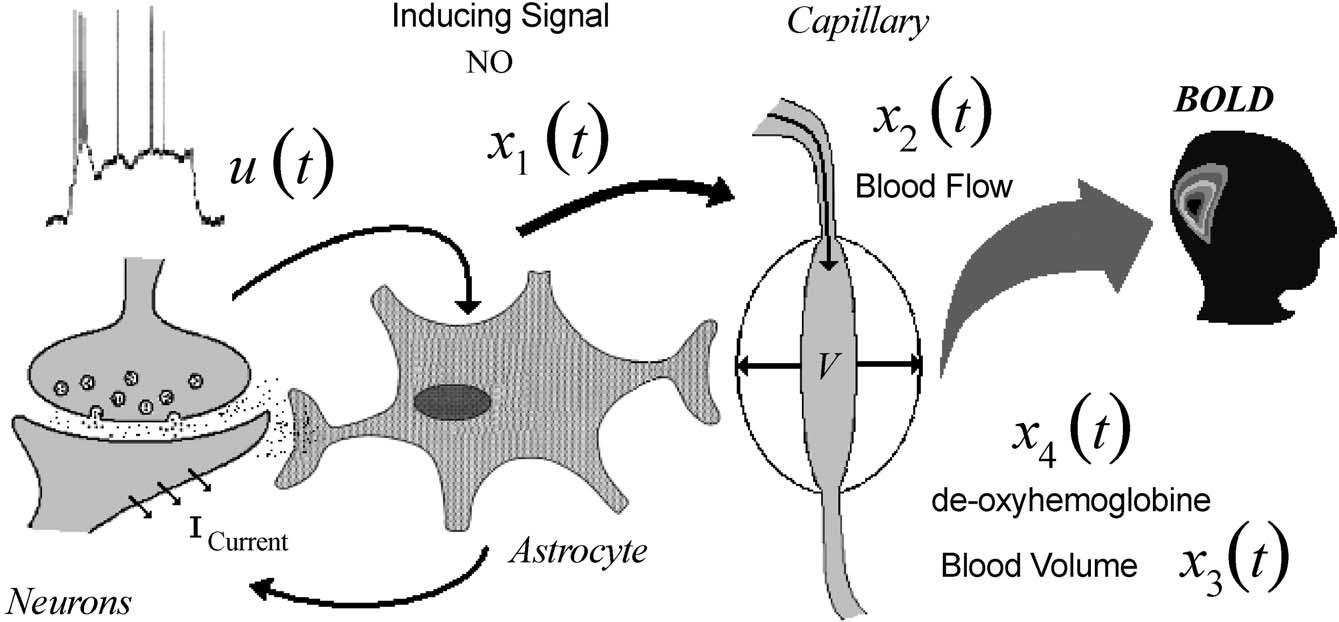
\includegraphics[width=10cm]{model}
\caption{
    \tiny
    \cite{Riera2003}
}
\end{figure}
\note{Rates from below 1 Hz to 5 to 6 Hundred Hz}
\note{Change in average firing rates increase metabolism and sympathetic response causes
        increased inflow of oxygenated blood.}
\note{In the version of the Balloon model I used, the flow is locked to metabolism.}
\note{According the balloon model this increases the local blood volume, and the outflow pressure.}
\note{So the signal is altered by changes in the ratio of Deoxyhemoglobin and Oxygenated Hemoglobin,
        which are a function of Volume and Oxygenation.}
\end{frame}

\begin{frame}{Time Changing Parameters}
    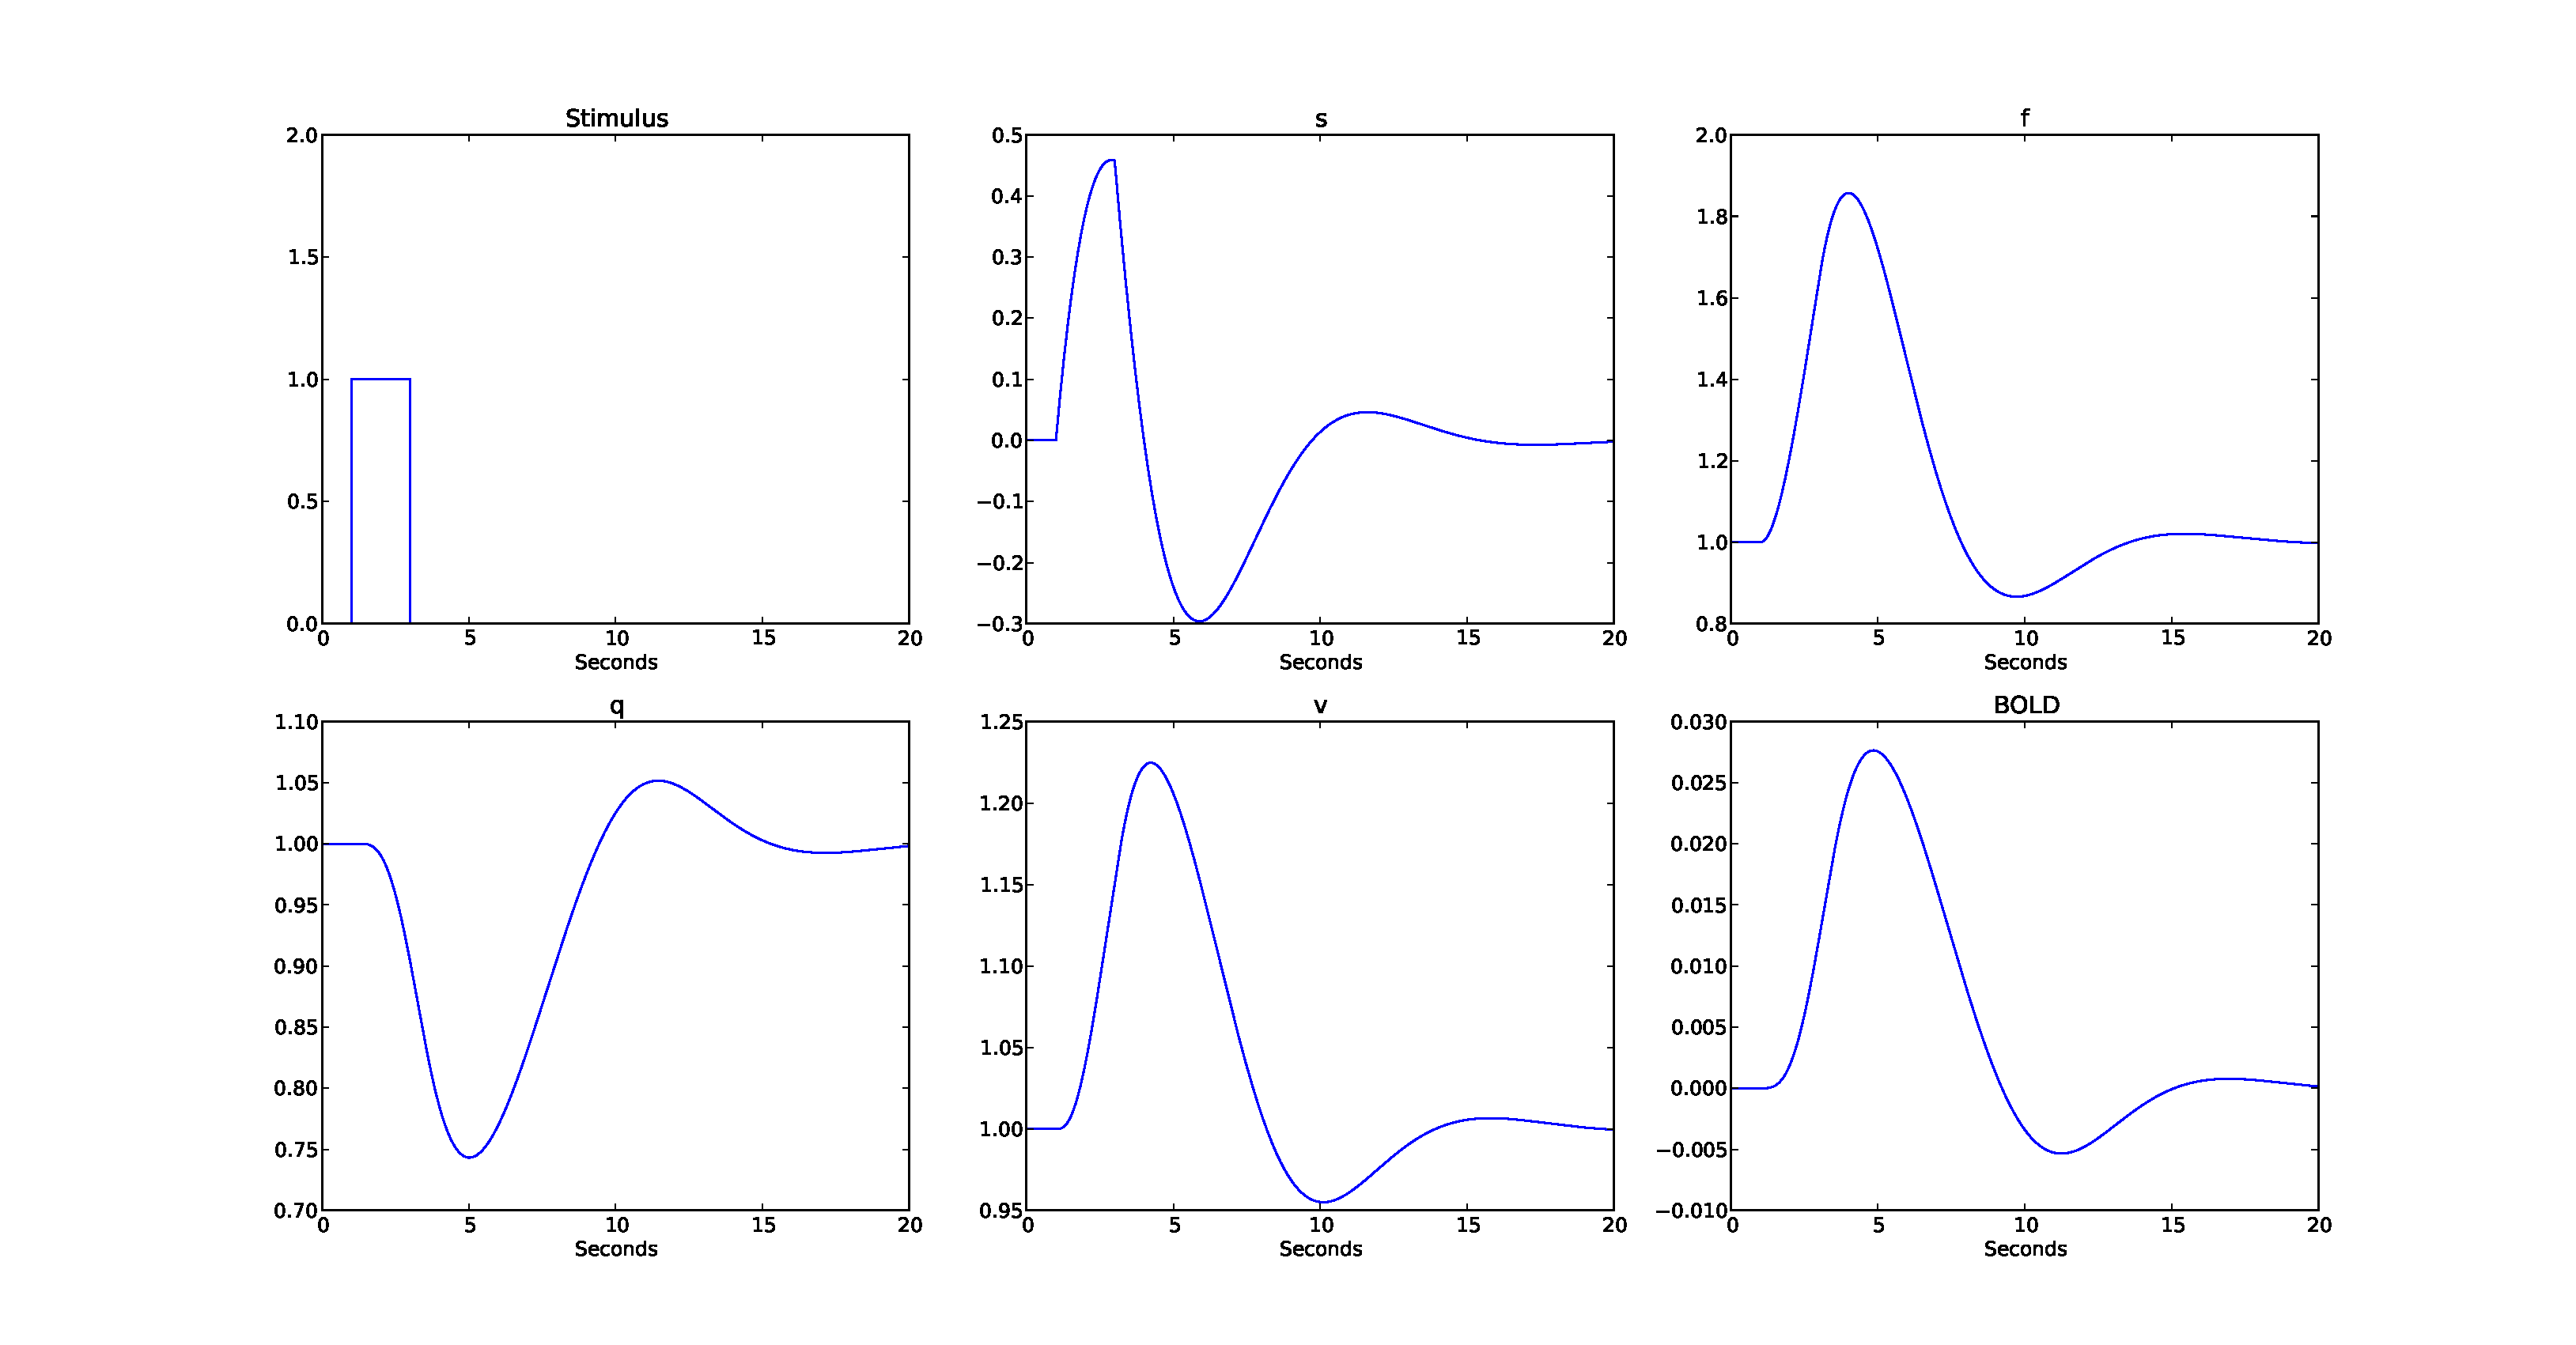
\includegraphics[clip=true,trim=3cm 1cm 3cm 1cm,width=\textwidth]{stateTS}
    \note{Should include a picture of the different parts of the BOLD signal}
\end{frame}

%more expansion of all the parameters
\begin{frame}{BOLD State Equations}
  \small
  \begin{itemize}
    \item Flow Inducing Signal
    $$\dot{s}(t) = \epsilon u(t) - s(t)/\tau_s - (f(t)-1)/\tau_f$$
    \item Normalized Cerebral Blood Inflow:
    $$\dot{f}(t) = s $$
    \item Normalized Cerebral Blood Volume:
    $$\dot{v}(t) = (1/\tau_0)( f(t) - v(t) ^ {1/\alpha}) $$
    \item Normalized Deoxyhaemoglobin Content:\\
    $$\dot{q}(t) = \frac{1}{\tau_0}\left(\frac{f(t)(1-(1-E_0)^{1/f(t)})}{E_0} -
            \frac{q(t)}{v(t)^{1-1/\alpha}}\right)$$
    \item Hemodynamic Response - BOLD Signal
    $$y(t) = V_0(a_1( 1 - Q(t)) - a_2(1 - V(t)))$$
  \end{itemize}
  \note{System is dissipative:}
  \note{If no input is provided, it will rather quickly decay.}
  \note{Constant input leads to steady state response.}
  \note{First term in $\dot{q}$ is the metabolism term.}
  \note{Outflow is the $v^{1/\alpha}$ term}
  \note{Significant nonlinearity.}
\end{frame}

\section{Potential Approaches}
\begin{frame}{Approximate Method}
  \begin{itemize}
    \item 2nd Order Volterra Kernel \cite{Friston2000}
    \note{Quadratic Approximation}
    \begin{itemize}
        \item Quadratic Convolution used to approximate Jacobian Matrix.
        \note{Because of the nonlinearities in the BOLD model, step size for
                integrating would otherwise be extremely small}
        \item Volterra approximation quality is not known.
    \end{itemize}
    \note{Volterra Approximation depends on sparsity etc}
    {\footnotesize
    $$y(t) = k_0 + \int_{-\infty}^{\infty} k_1(s_1) x(t-s_1) ds_1
        + \int_{-\infty}^{\infty} k_2(s_1,s_2) x(t-s_1)x(t-s_2) ds_1 ds_2$$
        \note{Its possible this isn't even knowable}
    }
    \item Canonical Hemodynamic Response Function
    \note{Linear Approximation}
    \begin{itemize}
        \item No Parameters Estimated
        \item Maximum Likelihood Possible
        \item Inflexible - even to changes in onset time
    \end{itemize}
    \begin{center}
    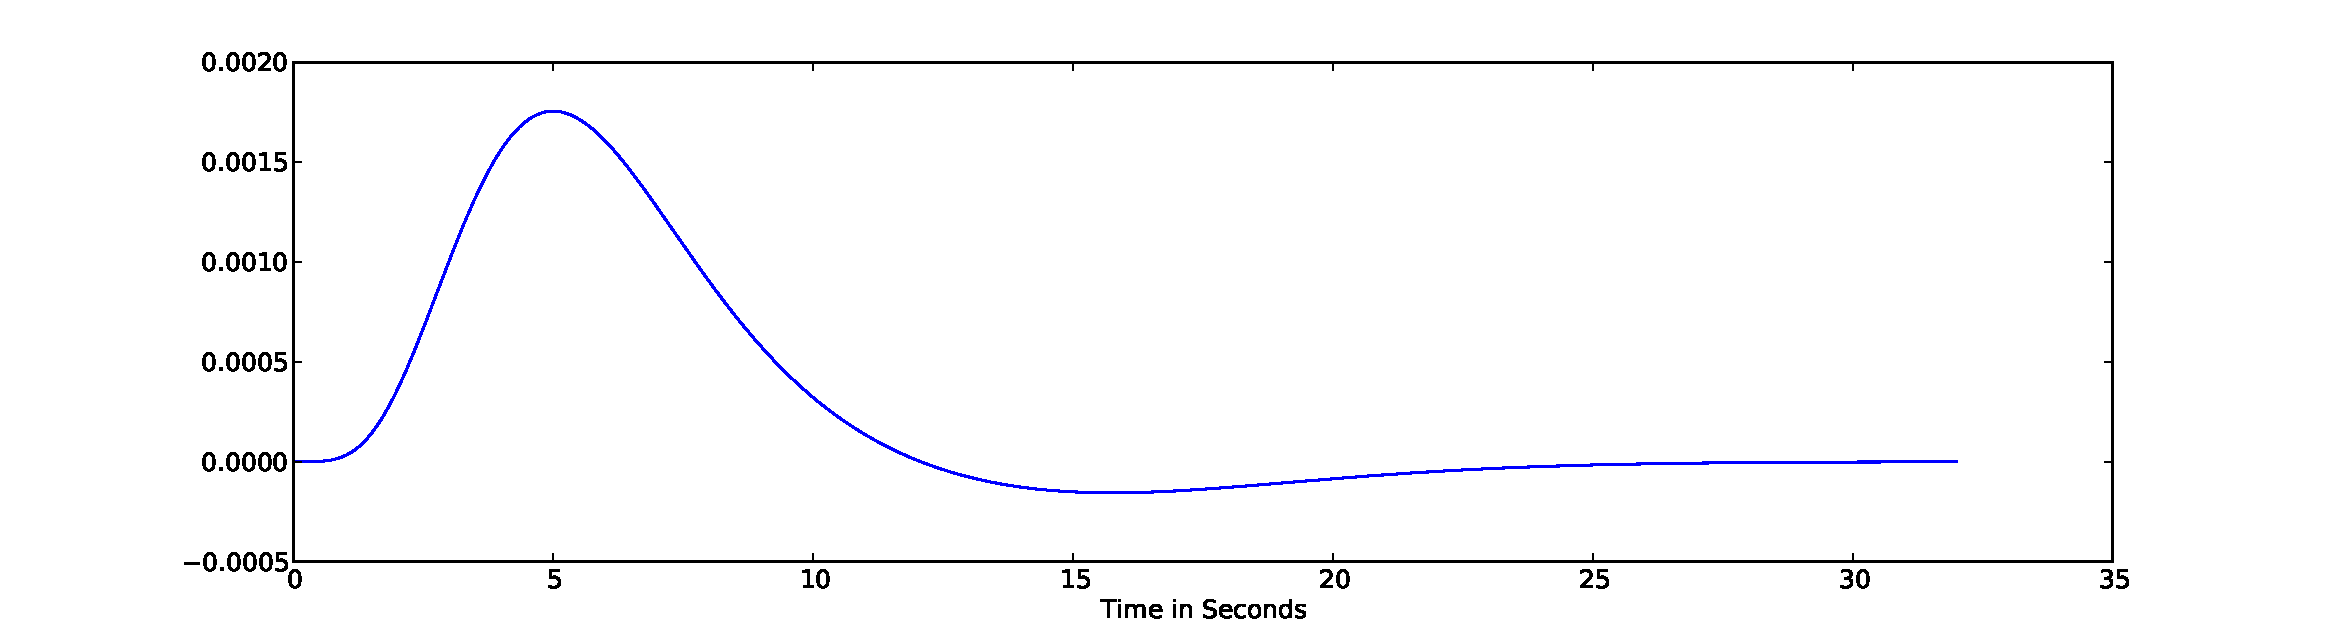
\includegraphics[clip=true,trim=4.88cm 0cm 5cm 1.5cm,height=2.7cm,width=8cm]{HRF}
    \end{center}
    
  \end{itemize}
\end{frame}

\begin{frame}{Nonlinear Modeling}
\begin{itemize}
    \item Local Linearization filter \cite{Riera2003}
     \note{Jacobian of the $\dot{x}$ is available, making gradient descent possible}
    \item Genetic Algorithms and Simulated Annealing \cite{Vakorin2007}
     \note{Genetic Algorithms were used to optimize spike points, simulated annealing for the parameters}
    \item Particle Filters to estimate $P(X_t | \Theta, Y_T)$ \cite{Murray2009}
    \begin{itemize}
        \item ML estimate of $\Theta$ based on $P(X_t | \Theta, Y_t)$ \cite{Johnston2007}
         \note{Particle Filter used to estimate states, ML of parameters based on the posterior of states and so on}
    \end{itemize}
    \item Unscented Kalman Filter to estimate parameters \cite{Hu2009}
    \item Direct Particle Filter, used in this work
     \note{Technically Kalman Filters and Particle Filters are Bayesian Filters}
     \note{Essentially filtering out inconsistent parameters.}
\end{itemize}
\end{frame}

\section{Particle Filter}
\begin{frame}{Construction}
\begin{itemize}
    \item Initialize Particles with Prior ($\alpha$):\\
        $$\{(x^i_0,w^i) : x^i_0 \sim \alpha(X), w^i = 
                \frac{1}{N_p}, i \in \{1, 2, ... , N_p\} \}$$
        $$\alpha(X) \stackrel{\text{\tiny{k=0}}}{\approx} P(x_k) 
                = \sum_{i=0}^{N_p} w^i\delta(x_k - x^i_k ) dx$$
    \item Particle Weights at time $t_k$:\\
        $$w^i_k \propto \frac{P(x^i_{0:k} | y_{0:k})}{q(x^i_{0:k} | y_{0:k})}$$
      \note{$q$ is the density/location of the particle}
      \note{$p$ is the actual probability }
    \item Adding Measurements:\\
        $$w^i_k \propto & w^i_{k-1}P(y_k| x_k) $$
      \note{Because of the proportion, note that the weights do not
            have to integrate to 1, and can be extremely large or extremely small}
\end{itemize}
\end{frame}

\begin{frame}{Particle Filter Algorithm}
\footnotesize
\begin{algorithm}
\begin{algorithmic}
\STATE Initialize Particles:
\FOR{$i$ : each of $N_p$ particles }
    \STATE $x^i_0  \sim \alpha(X)$
    \STATE $w^i_0 = \frac{1}{N_p}$
\ENDFOR
\FOR{$k$ : each measurement}
    \FOR{$i$ : each particle }
        \STATE $x^i_k = x^i_{k-1} + \int_{t-1}^t f(x(\tau), u(\tau)) d\tau $
        \STATE $w^i_k = w^i_{k-1}P(y_k | x_k)$
    \ENDFOR
    \STATE Calculate $N_{eff}$ 
    \IF{$N_{eff} < N_R$ (recommend $N_R = min(50, .1N_p)$ )}
        \STATE Regularized Resample 
    \ENDIF
\ENDFOR

\STATE At $t + \Delta t$, $t \in T$, $P(x(t+\Delta t)) \approx 
\sum_{i=1}^{N_p} w_i(t)\delta\left(x - (x_i(t) + \int_t^{t+\Delta t} f(x(\tau), u(\tau)) d\tau) \right)$
 \end{algorithmic}
 \end{algorithm}
\end{frame}

\begin{frame}{Details and Example}
  \begin{columns}
    \begin{column}{.55\textwidth}
        \begin{itemize}
            \item Non-parametric
            \item Model based
            \item Online
            \item Provides Full Posterior Probability
            \item Non-trivial computation cost
            \item Regularized Particle Filter Used
        \end{itemize}
    \end{column}
    \begin{column}{.45\textwidth}
        \begin{figure}
          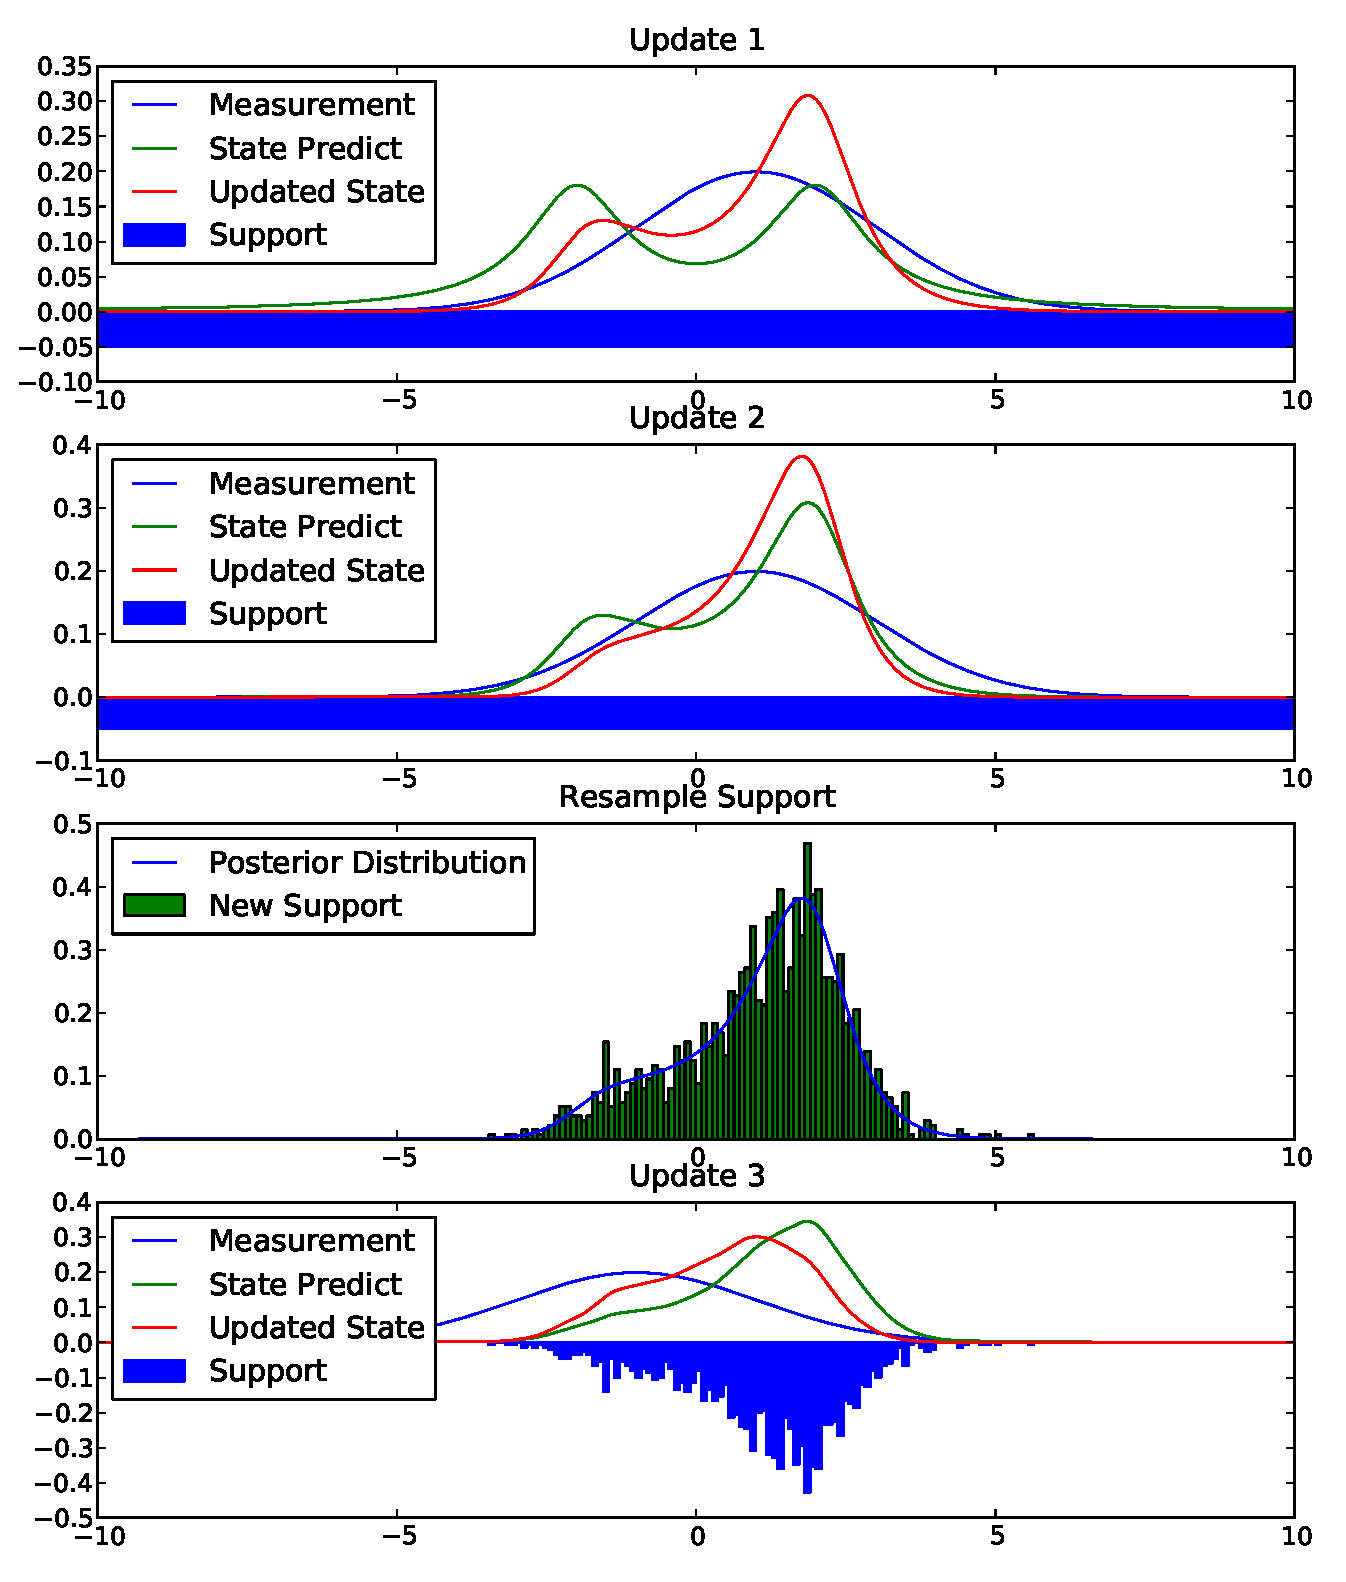
\includegraphics[width=\textwidth]{particle_filter}
        \end{figure}
    \end{column}
    \end{columns}
\end{frame}

\section{Methods}
\begin{frame}{FMRI Noise}
\centering

Resting State Noise

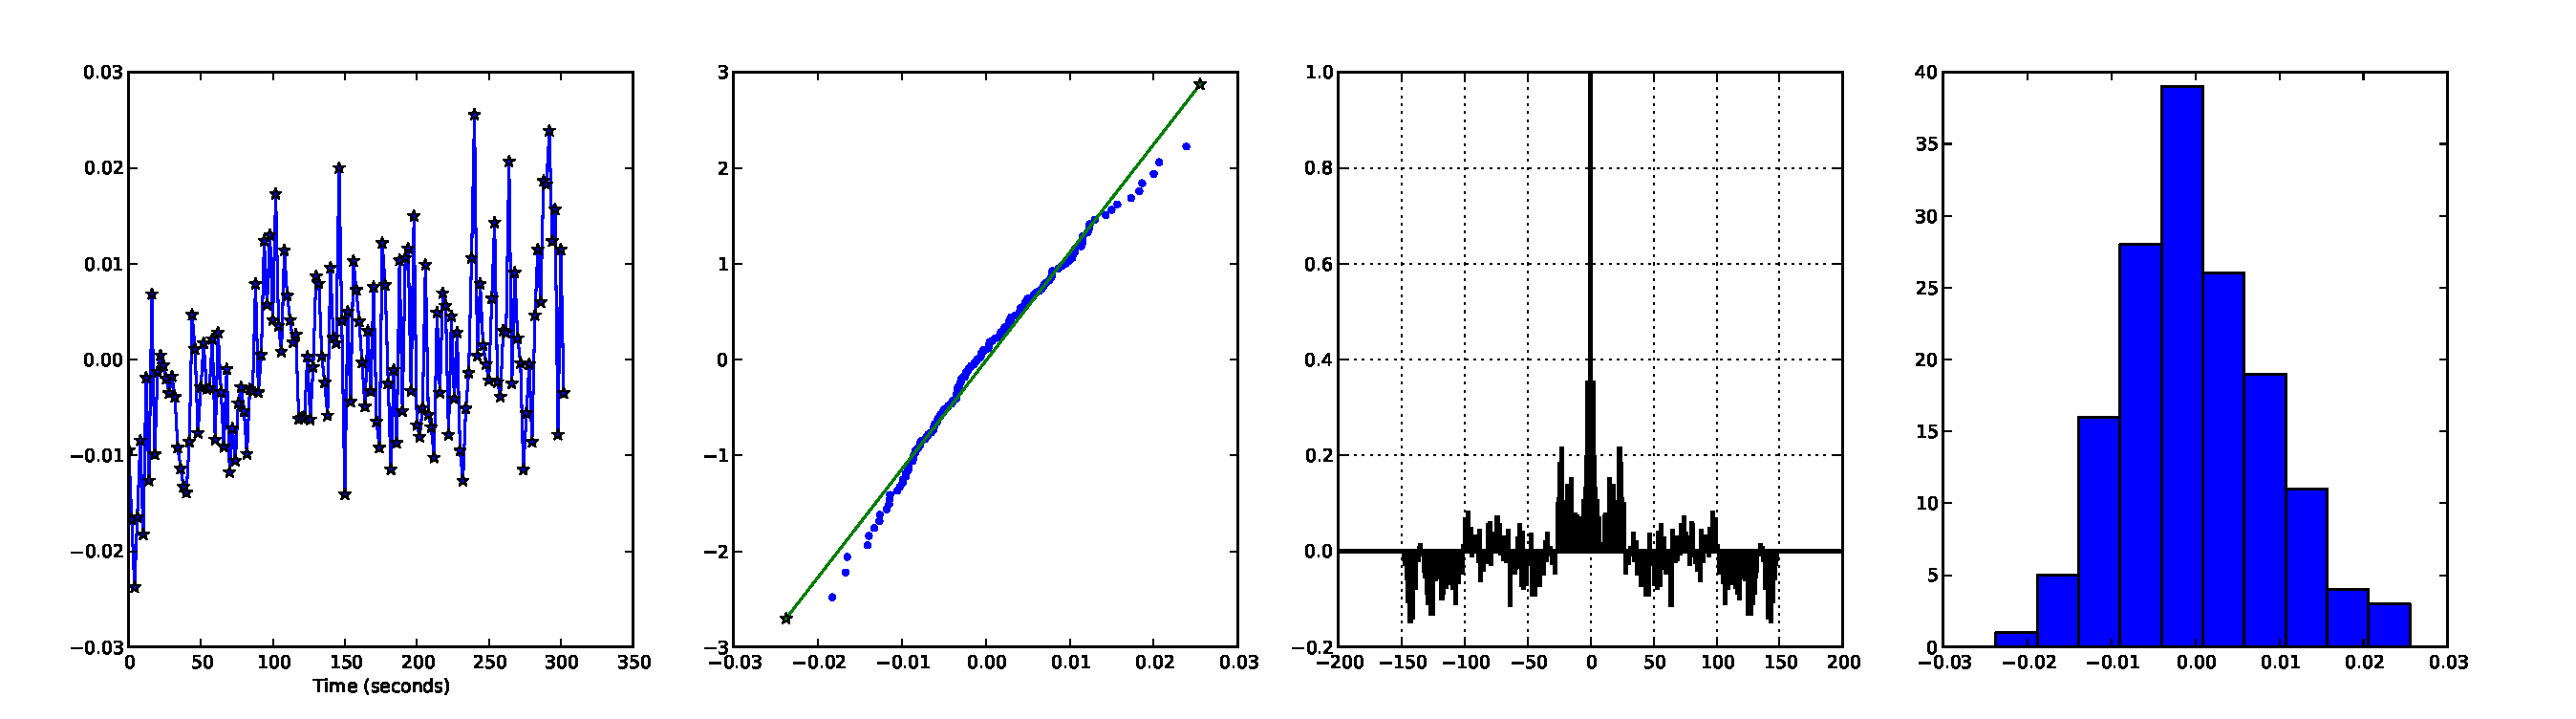
\includegraphics[trim=3cm 0cm 3cm 0cm,width=.75\textwidth]{noise2_0009_22_38_23}

Resting State Noise Steps

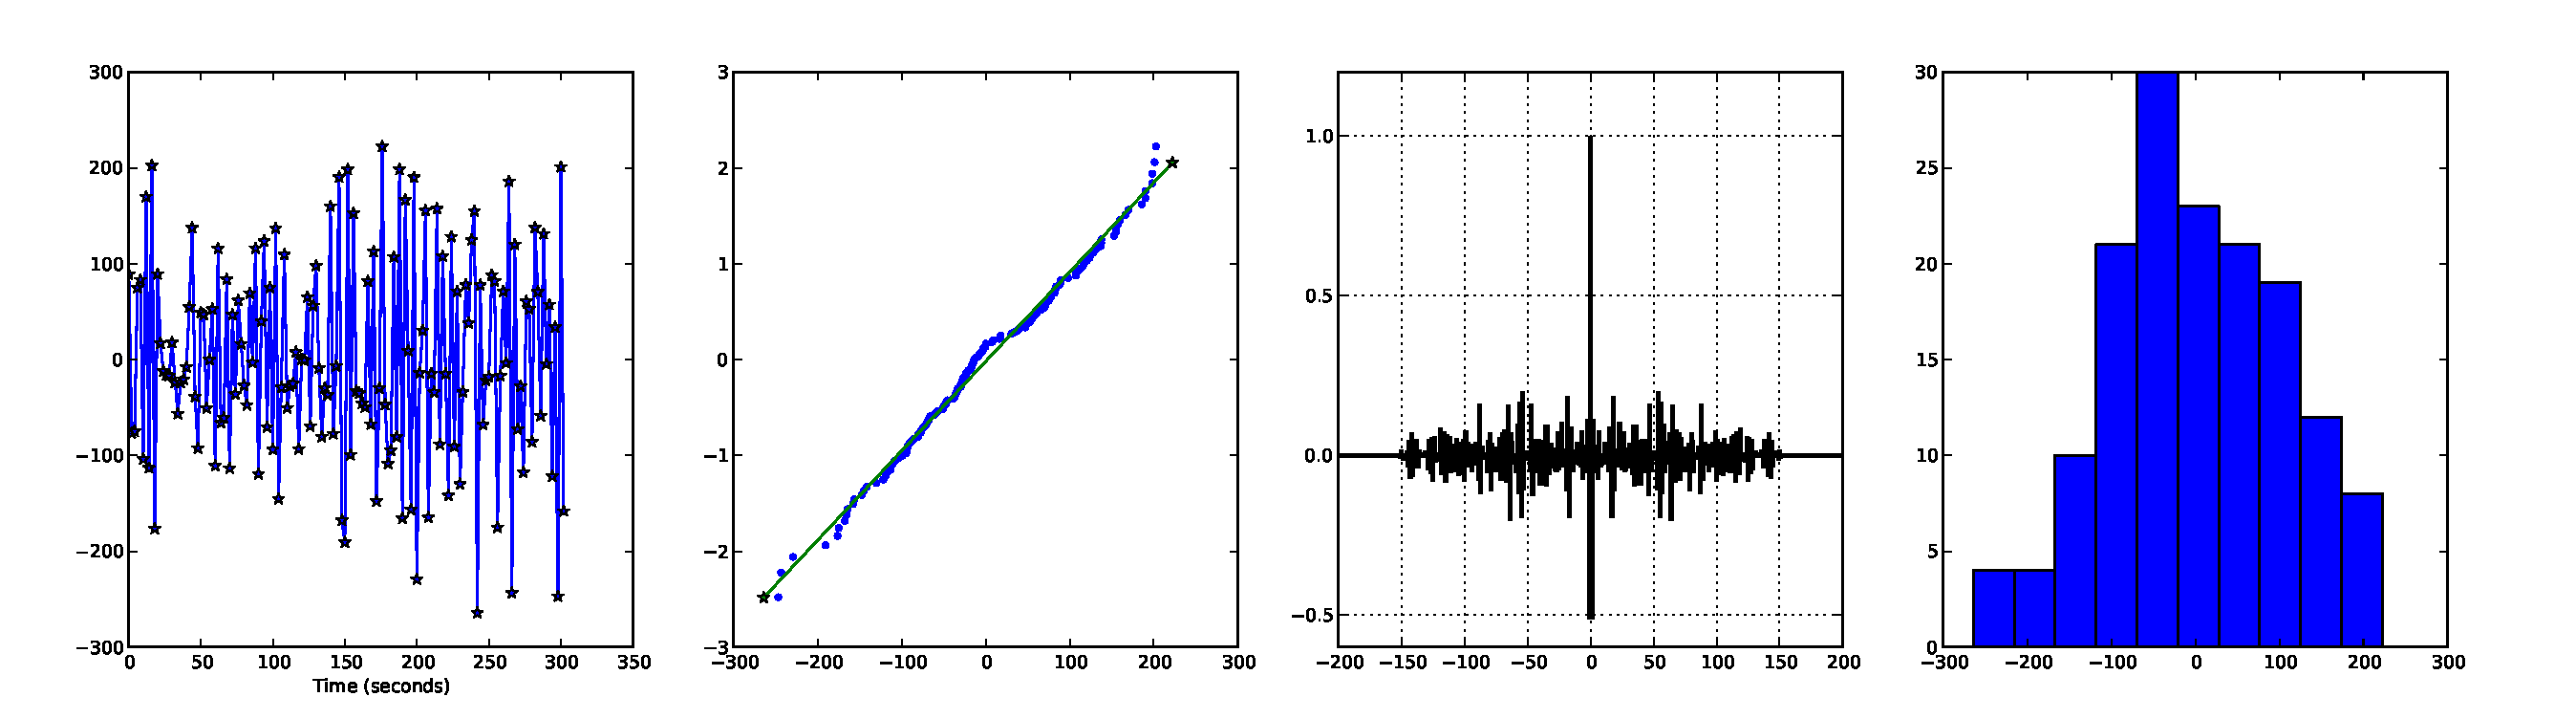
\includegraphics[trim=3cm 0cm 3cm 0cm,width=.75\textwidth]{noise2_0009d_22_38_23}

\note{Tanabe 2002 \autoref{Tanabe2002} 10-15\% of voxels exhibit significant drift}
\note{Occurs in Cadavers.}
\end{frame}

\begin{frame}{Preprocessing}
  \begin{columns}
    \begin{column}{.6\textwidth}
        \begin{itemize}
            \item Drop Inital Volumes (9, $18.9$s)
            \item Realign Over Time
            \item Detrend (SPM uses $0.0078125 Hz$ cut off)
            \item Gaussian Smoothing (SPM Only)
            \begin{itemize}
                \item Imposes Gaussianity
                \item Increases SNR
                \item Reduces Bonferroni Correction Requirement
            \end{itemize}
        \end{itemize}
    \end{column}
    
    \begin{column}{.4\textwidth}
        \includegraphics[width=\textwidth]{preprocess}
    \end{column}
  \end{columns}
\end{frame}

\section{Results}
\begin{frame}{Long Run Results}
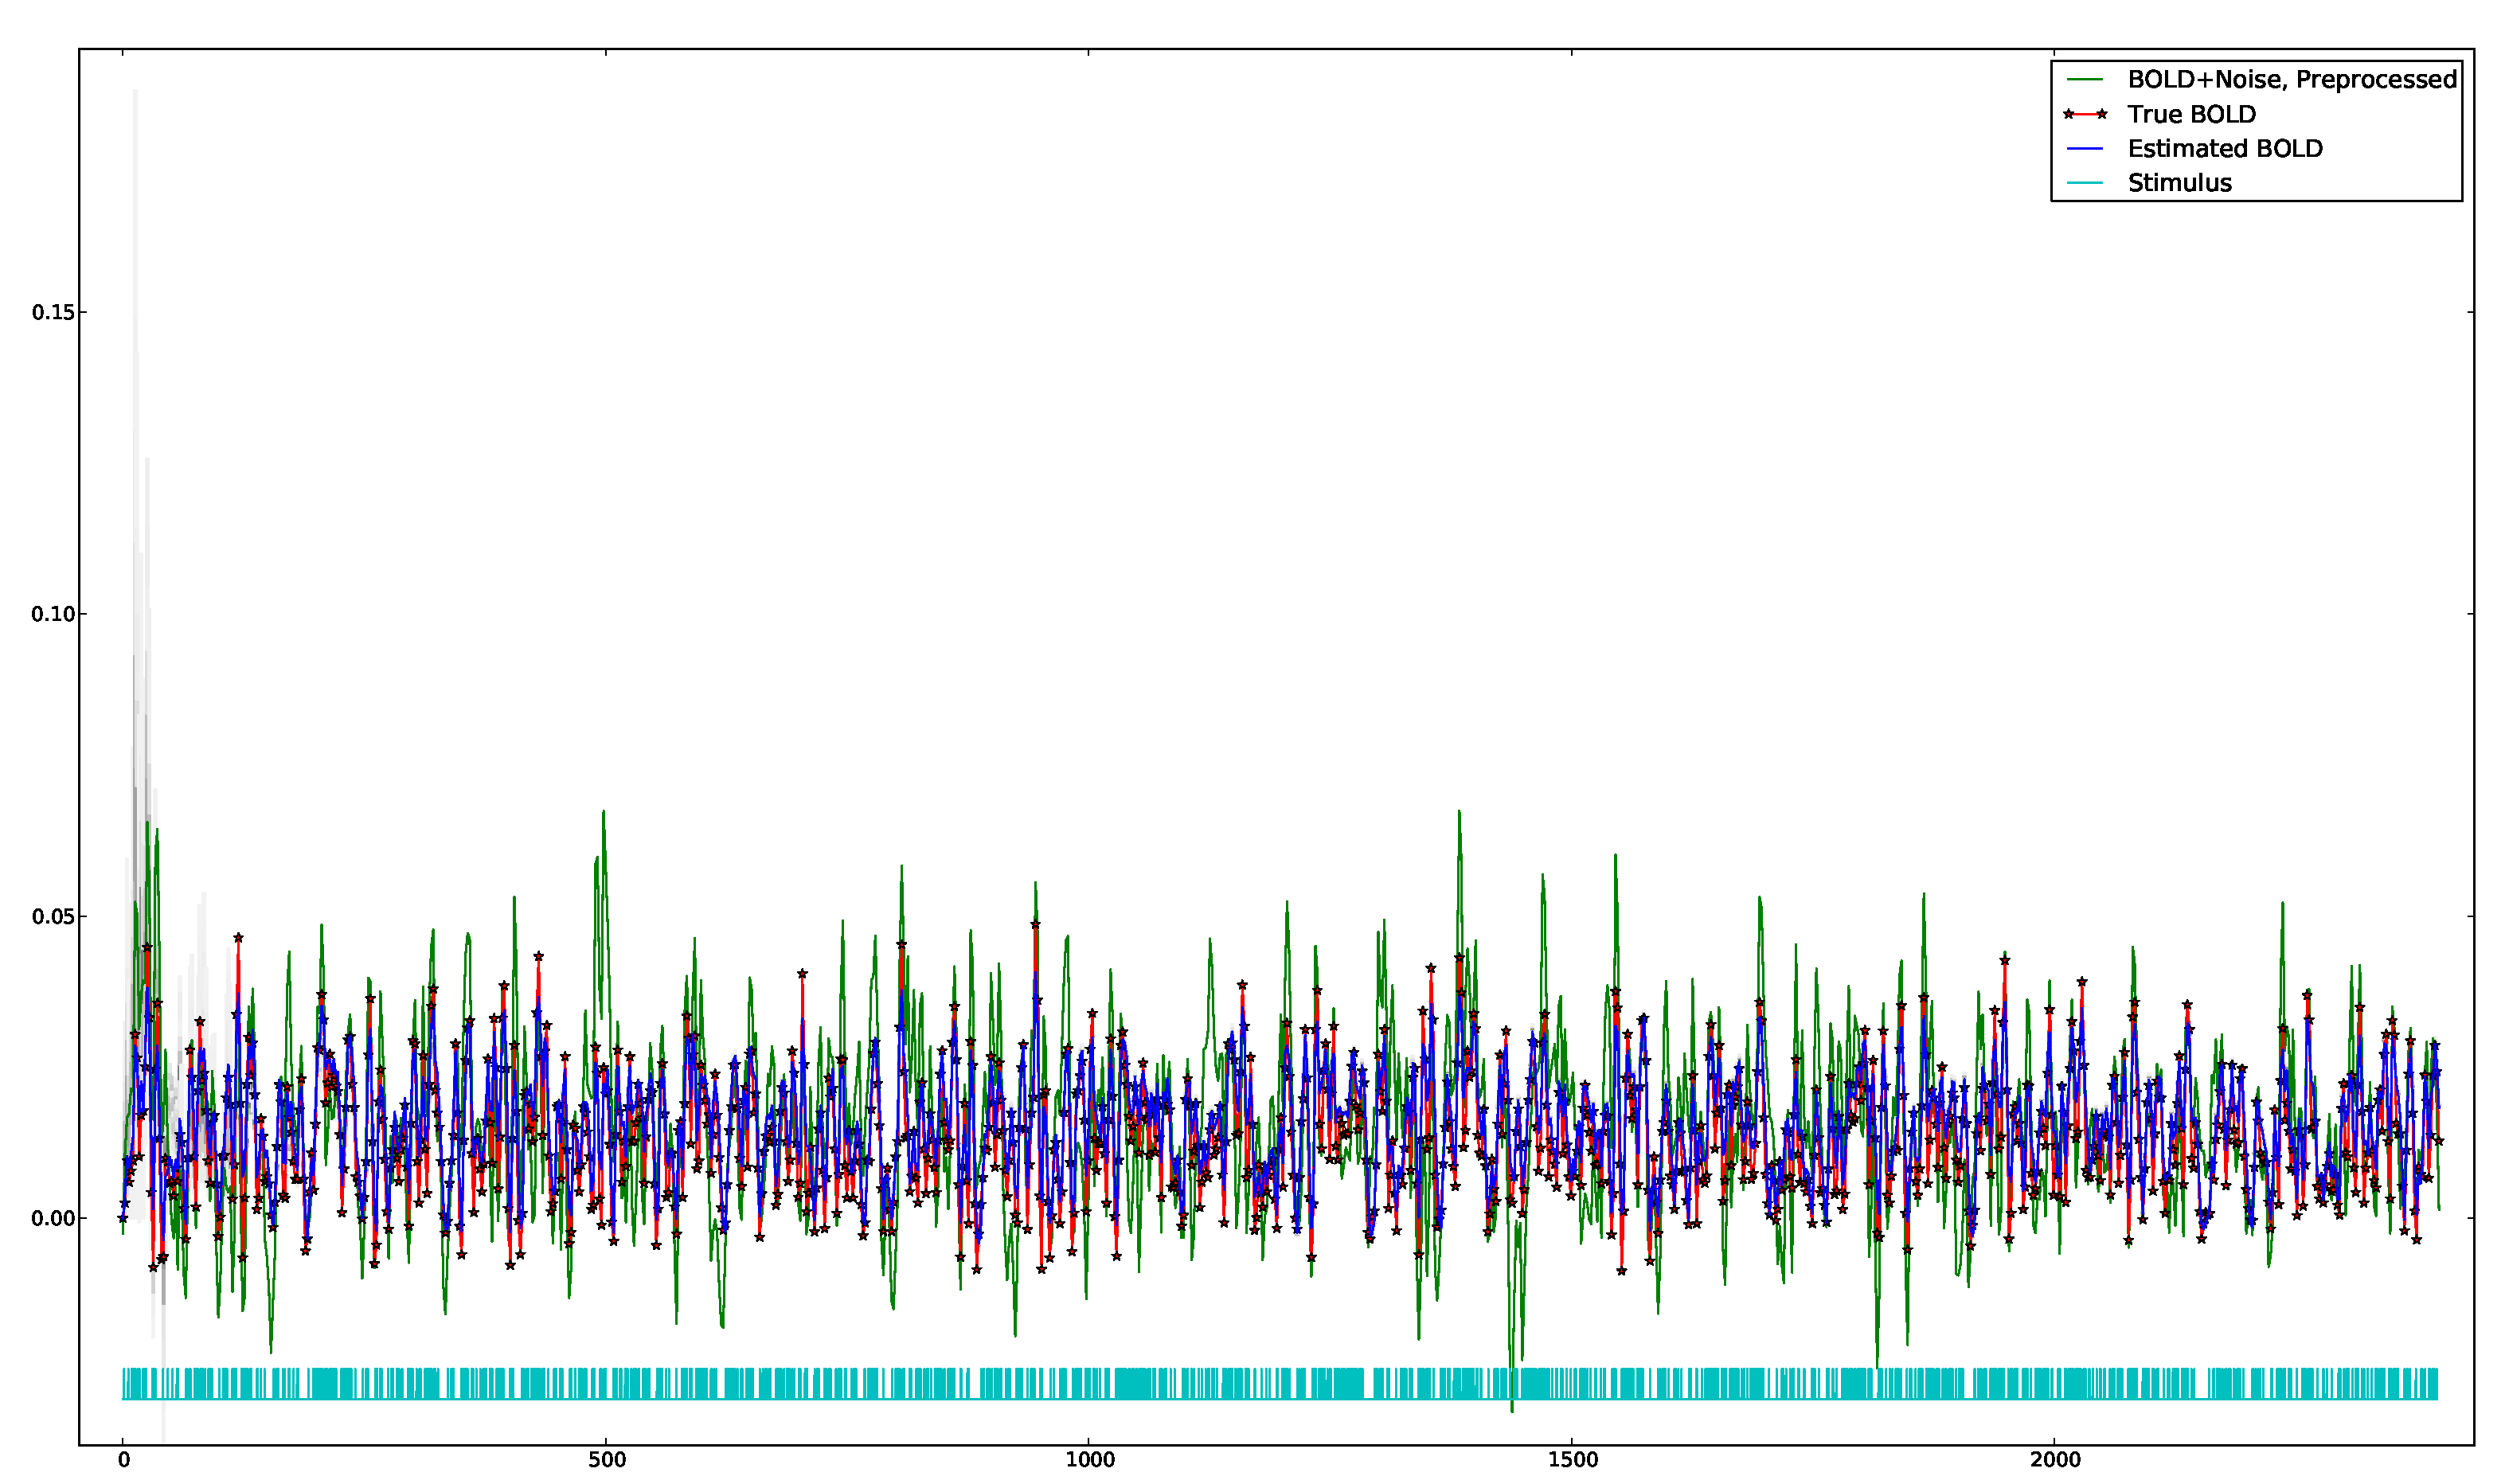
\includegraphics[width=\textwidth]{long_converge}
\note{Bars drop well before the end}
\note{Mean is good estimator}
\note{Mean comes very close to truth}
\end{frame}

\begin{frame}{Long Run Correlation}
\centering
Estimated Parameter Covariance 

\begin{table}[t]
\tiny
\begin{tabular}{|c | c  c  c  c  c  c  c |}
\hline
  & $\tau_0$ & $\alpha$ & $E_0$    & $V_0$    & $\tau_s$ & $\tau_f$ & $\epsilon$ \\
\hline
\rowcolor[gray]{.8} $\tau_0$  & 0.0004334 & 5.2e-05 & -6.95e-05 & 3.3e-06 & 0.0001628 & -2e-07 & 0.0001798 \\
$\alpha$                      & 5.2e-05 & 7.9e-06 & -6.4e-06 & 3e-07 & 1.04e-05 & -1.92e-05 & 2.58e-05 \\
\rowcolor[gray]{.8} $E_0$     & -6.95e-05 & -6.4e-06 & 1.9e-05 & -9e-07 & -4.11e-05 & -3.24e-05 & -3.92e-05 \\
$V_0$                         & 3.3e-06 & 3e-07 & -9e-07 & 1e-07 & 1.1e-06 & 9e-07 & 1e-06 \\
\rowcolor[gray]{.8} $\tau_s$  & 0.0001628 & 1.04e-05 & -4.11e-05 & 1.1e-06 & 0.0001589 & 0.0001518 & 7.88e-05 \\
$\tau_f$                      & -2e-07 & -1.92e-05 & -3.24e-05 & 9e-07 & 0.0001518 & 0.0002966 & -2.34e-05 \\
\rowcolor[gray]{.8} $\epsilon$& 0.0001798 & 2.58e-05 & -3.92e-05 & 1e-06 & 7.88e-05 & -2.34e-05 & 0.0001966 \\
\hline
\end{tabular}
\label{tab:long_cov}
\end{table}

Estimated Parameter Correlation 

\begin{table}[t]
\tiny
\begin{tabular}{|c | c  c  c  c  c  c  |}
\hline
  & $\tau_0$ & $\alpha$ & $E_0$    & $V_0$    & $\tau_s$ & $\tau_f$  \\
\hline
\rowcolor[gray]{.8} $\tau_0$  & & & & & & \\
$\alpha$                      & 0.889884 & & & & & \\
\rowcolor[gray]{.8} $E_0$     & -0.7661395 & -0.5230723 & & & & \\
$V_0$                         & 0.6244049 & 0.4239271 & -0.7964774 & & & \\
\rowcolor[gray]{.8} $\tau_s$  & 0.6204843 & 0.295425 & -0.7481253 & 0.3440421 & & \\
$\tau_f$                      & -0.0004259 & -0.3966881 & -0.4314174 & 0.1962954 & 0.6990775 & \\
\rowcolor[gray]{.8} $\epsilon$& 0.6158116 & 0.6558179 & -0.641348 & 0.2846632 & 0.4458142 & -0.097079 \\
\hline
\end{tabular}
\note{Correlation of parameter estimates at the end of 
            \autoref{fig:long_converge}.}
\label{tab:long_corr}
\end{table}
\end{frame}

\begin{frame}{Short Run Results A}
\begin{center}
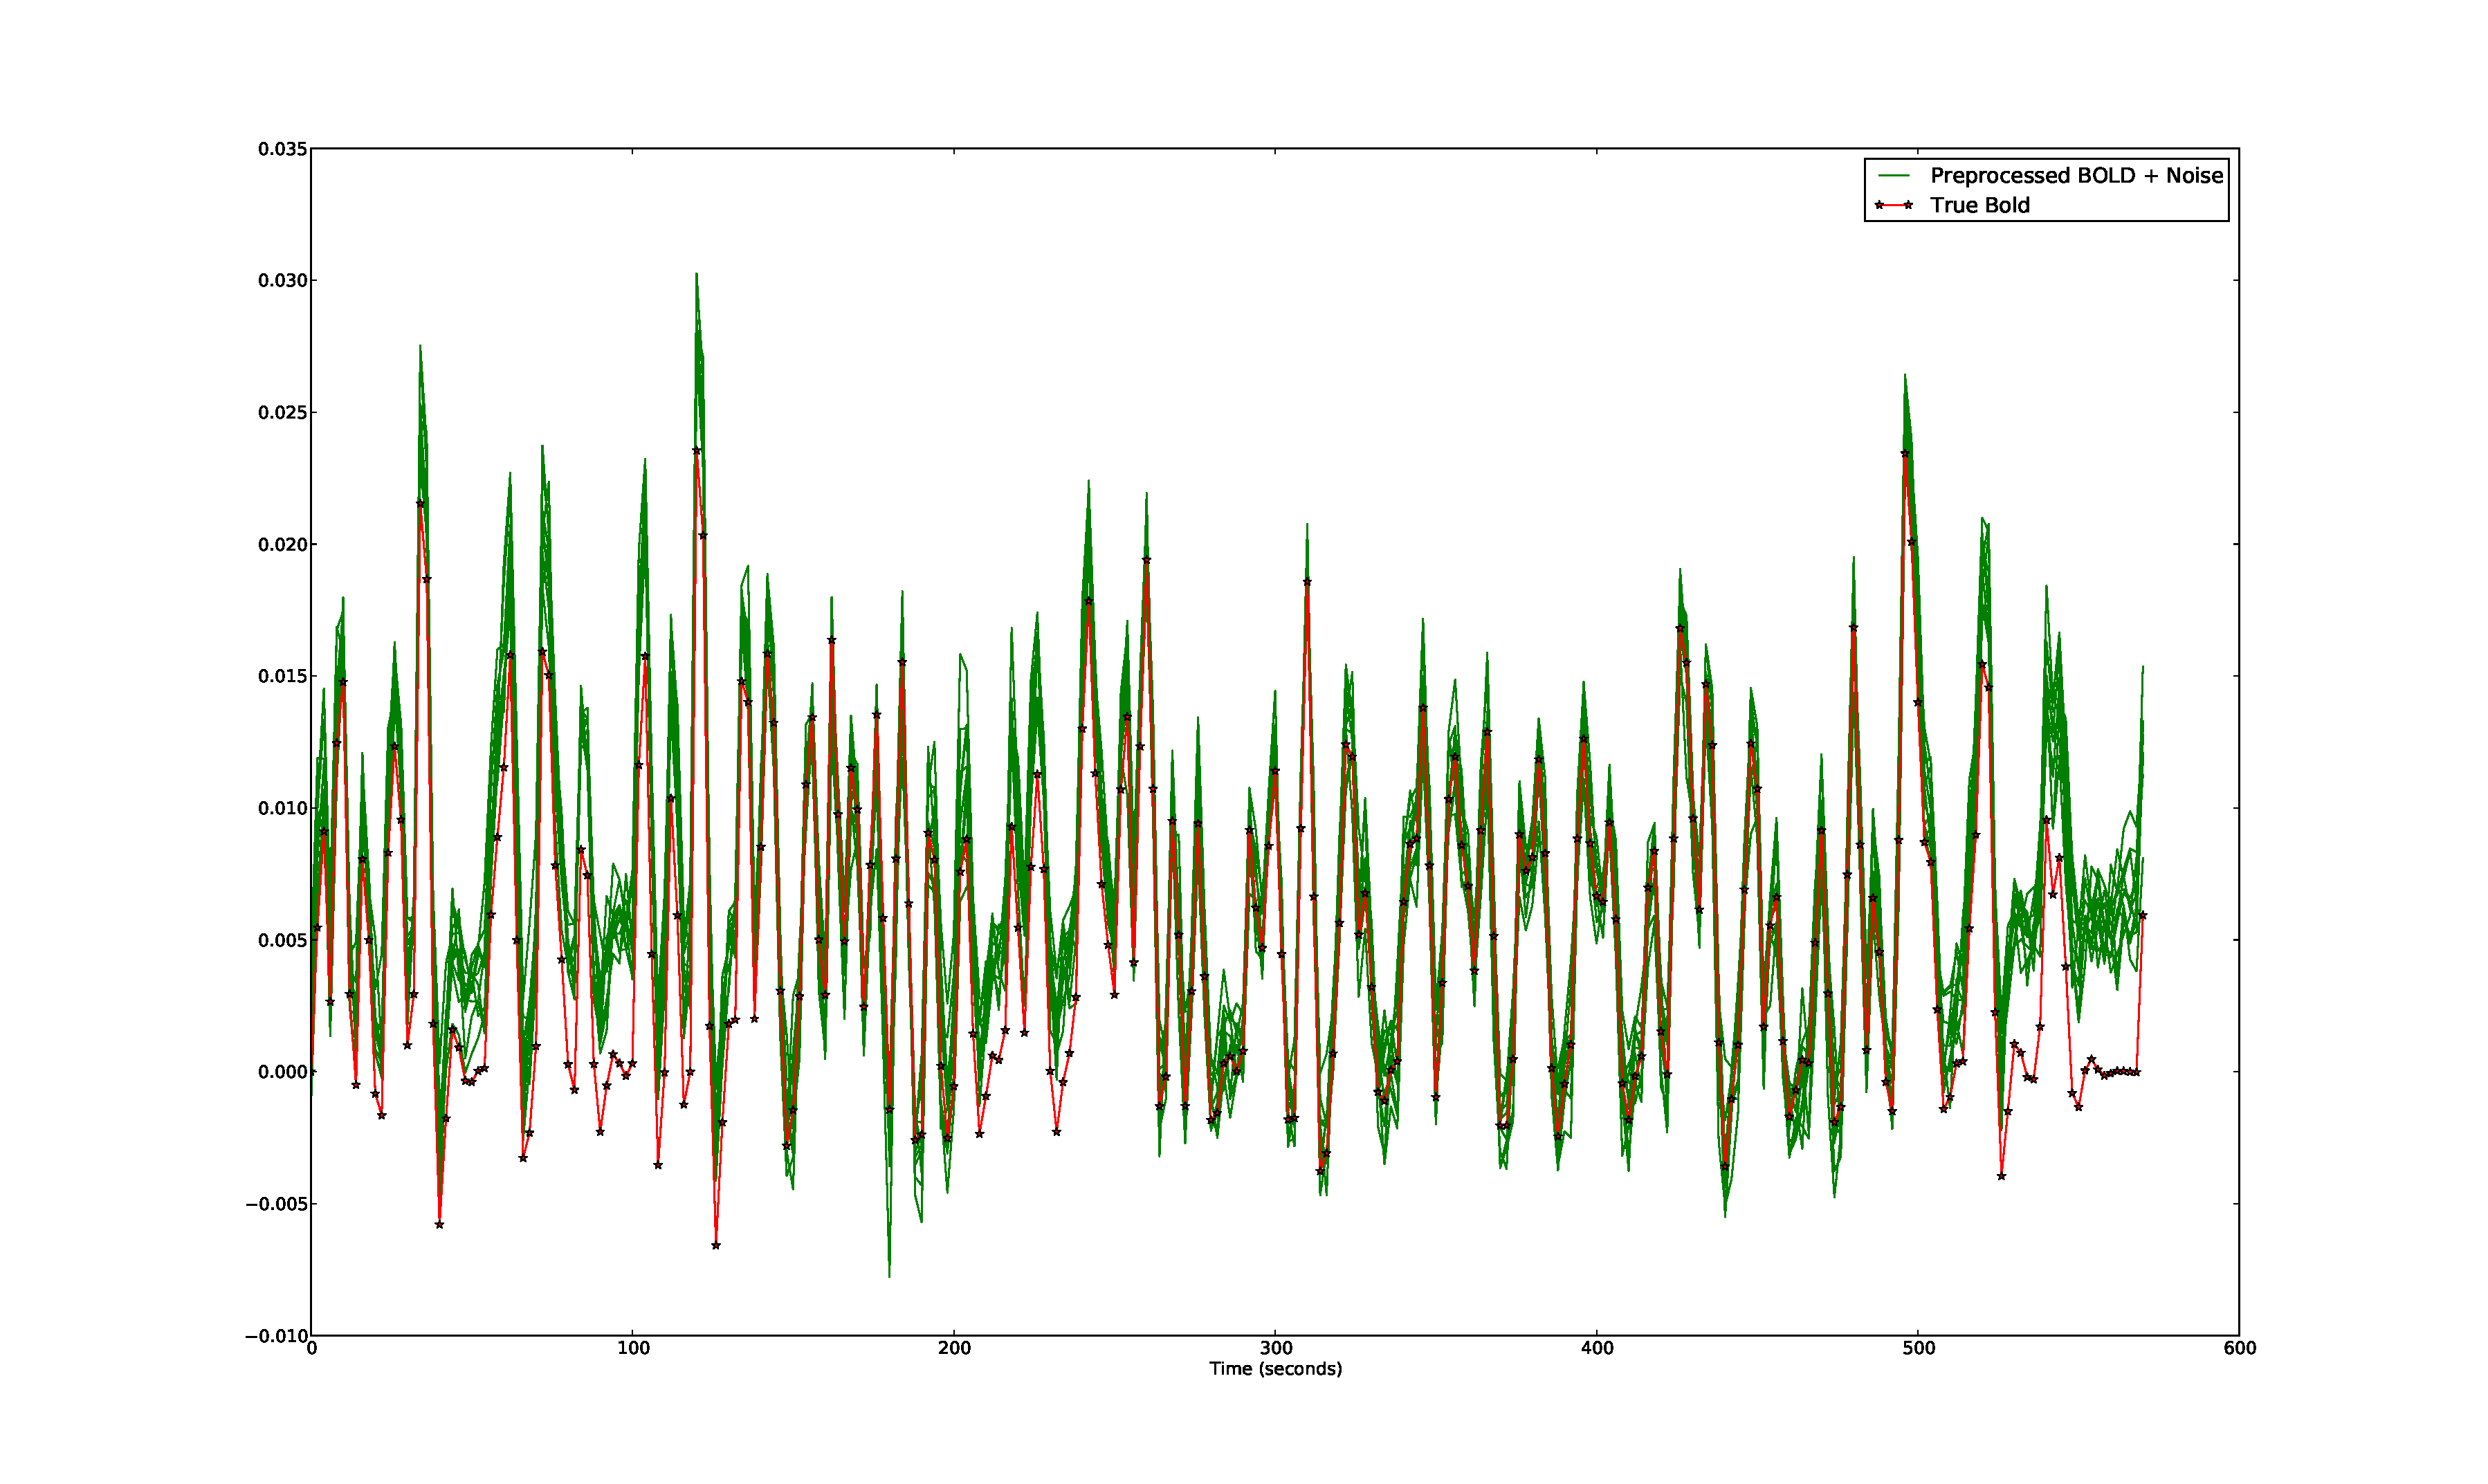
\includegraphics[clip=true,trim=6cm 2cm 5cm 3.5cm,width=.9\textwidth]
            {preprocessed_lownoise}
\end{center}
\end{frame}

\begin{frame}{Short Run Results B}
\begin{center}
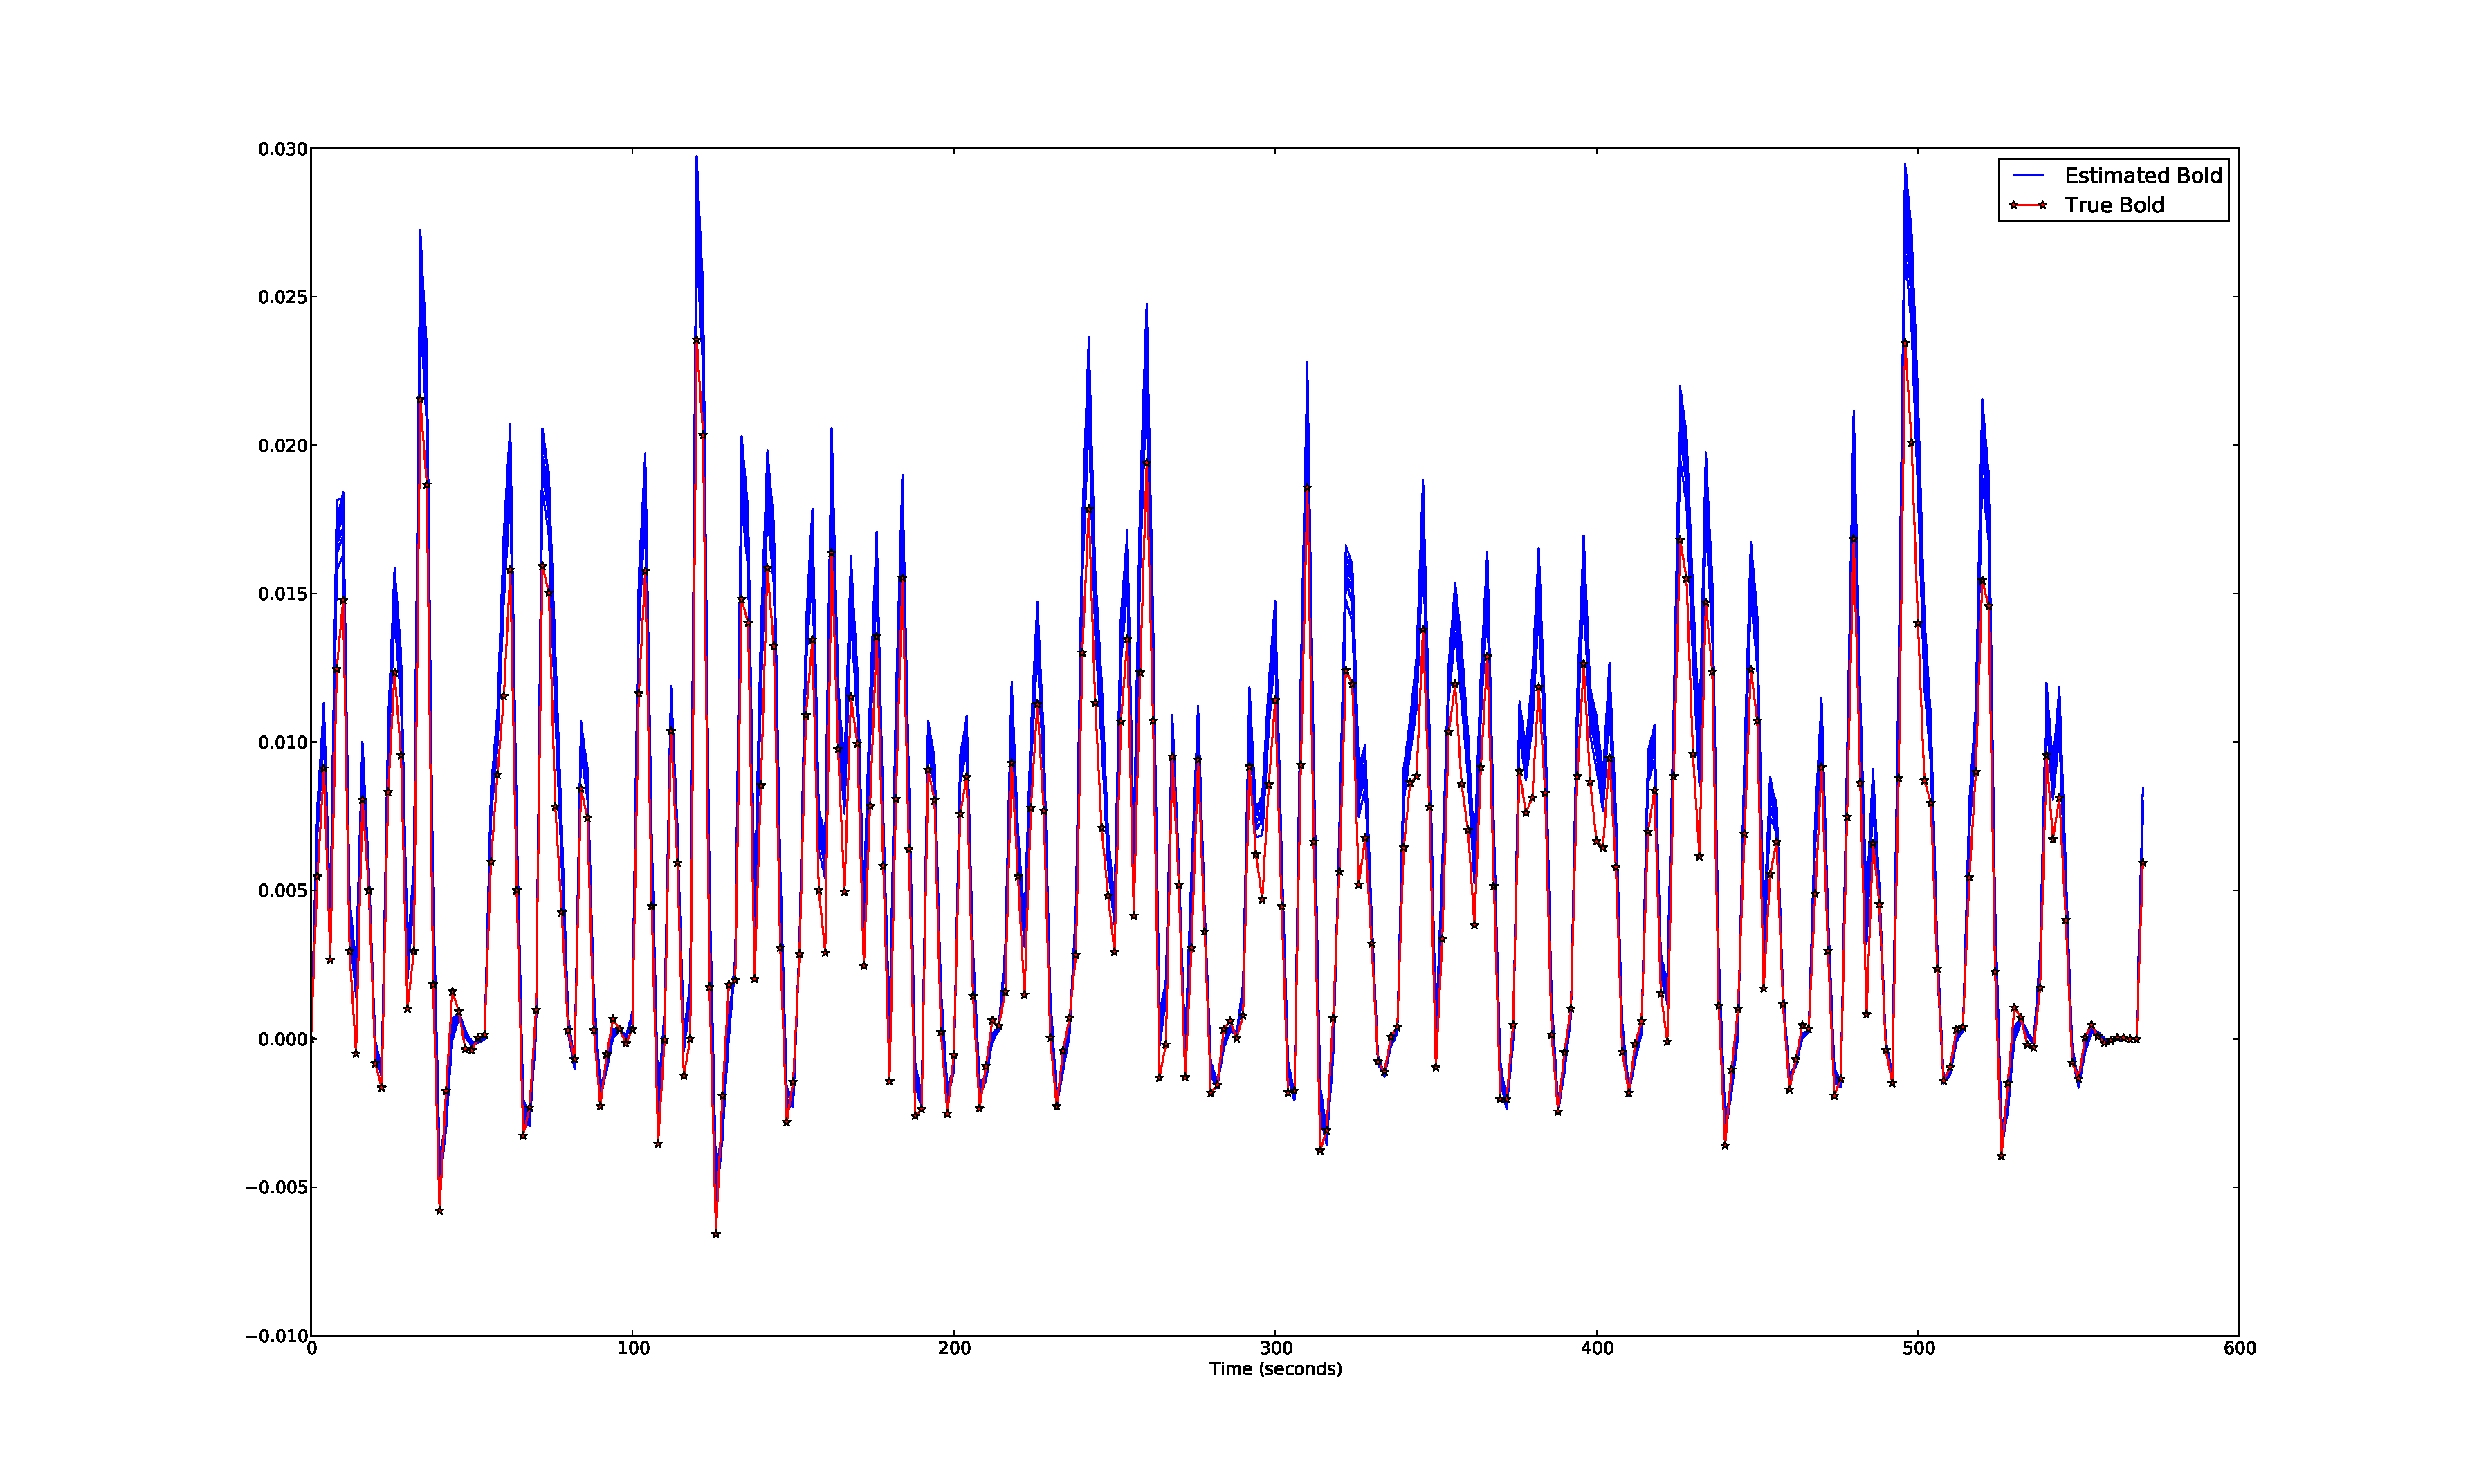
\includegraphics[clip=true,trim=6cm 2cm 5cm 3.5cm,width=.9\textwidth]
            {comparison_lownoise}
\end{center}
\end{frame}

\begin{frame}{Short Run Results C}
\begin{table}[t]
\centering
\resizebox{\textwidth}{!}{
\begin{tabular}{|c | c | c | c | c | c | c | c | c | c |}
\hline
$\tau_0$ & $\alpha$ & $E_0$    & $V_0$    & $\tau_s$ & $\tau_f$ & $\epsilon$  & $ \sum \tau $ & Error & Residual\\
\hline
\rowcolor[gray]{.8}
1.45 & 0.3 & 0.47 & 0.044 & 1.94 & 1.99 & 1.8  & 5.38 &  & \\
\hline
\hline
1.2221 & 0.3449 & 0.3346 & 0.0714 & 1.6045 & 2.2753 & 1.5945 & 5.1019 &  0.003211  & 0.00224\\
1.3749 & 0.3318 & 0.3630 & 0.0733 & 1.6408 & 2.1030 & 1.5763 & 5.1187 &  0.003055  & 0.00223\\
1.1660 & 0.3221 & 0.3406 & 0.0822 & 1.6477 & 2.3535 & 1.2452 & 5.1672 &  0.003289  & 0.00205\\
1.2318 & 0.3271 & 0.3403 & 0.0796 & 1.6270 & 2.1852 & 1.3033 & 5.0439 &  0.002847  & 0.00147\\
1.1832 & 0.3179 & 0.3472 & 0.0821 & 1.5496 & 2.2912 & 1.2782 & 5.0240 &  0.003006  & 0.00213\\
1.1424 & 0.334  & 0.3473 & 0.0737 & 1.6221 & 2.2908 & 1.4025 & 5.0553 &  0.002833  & 0.00184\\
1.3004 & 0.3596 & 0.3564 & 0.0768 & 1.5641 & 2.1323 & 1.6034 & 4.9968 &  0.003028  & 0.00255\\
1.2401 & 0.3460 & 0.3398 & 0.0891 & 1.6499 & 2.2366 & 1.2900 & 5.1265 &  0.003044  & 0.00238\\
1.1709 & 0.3274 & 0.3464 & 0.0826 & 1.5373 & 2.2826 & 1.3783 & 4.9909 &  0.003345  & 0.0027 \\
1.1897 & 0.3434 & 0.3355 & 0.0798 & 1.5358 & 2.3075 & 1.4277 & 5.0330 &  0.003175  & 0.00244\\
1.184 &  0.3405 & 0.3502 & 0.0892 & 1.6103 & 2.2793 & 1.1645 & 5.0735 &  0.002889  & 0.00188\\
\hline                                                                               
1.2187 & 0.3359 & 0.3456 & 0.0800 & 1.599 & 2.2488 & 1.3876 & 5.0665 & 0.003066     & 0.00217\\
\hline
\end{tabular}
}
\end{table}
\end{frame}

\begin{frame}{POSSUM Results: Activation}
\begin{figure}
\centering
\subfigure[Regions]{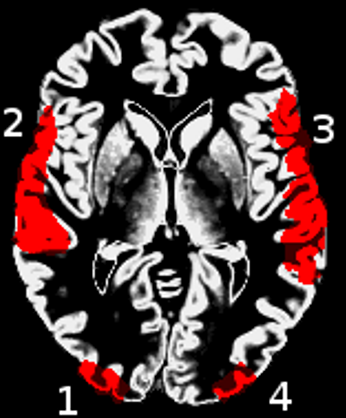
\includegraphics[height=.46\textheight]{simregions}}
\subfigure[Mutual Information]
{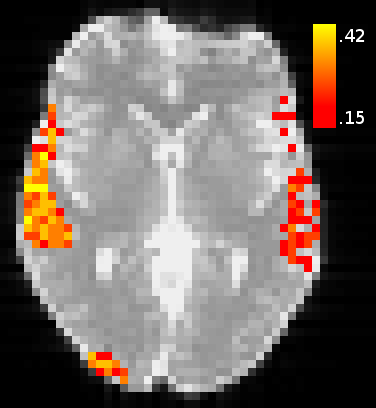
\includegraphics[height=.46\textheight]{sim_hm_15_6}}
\subfigure[SNR]{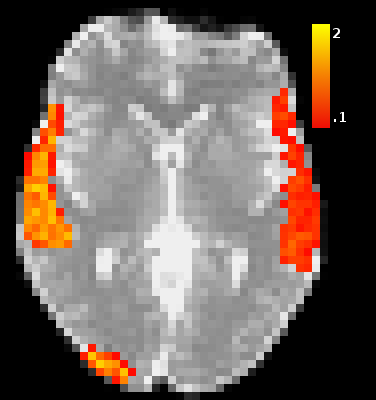
\includegraphics[height=.46\textheight]{snr_hm}}
\note{Mean SNR's Region 1: $0.8$, Region 2: $0.97$, and Region 3: $0.39$.}
\end{figure}
\end{frame}

\begin{frame}{POSSUM Results: Histogram}
\begin{figure}
%\centering
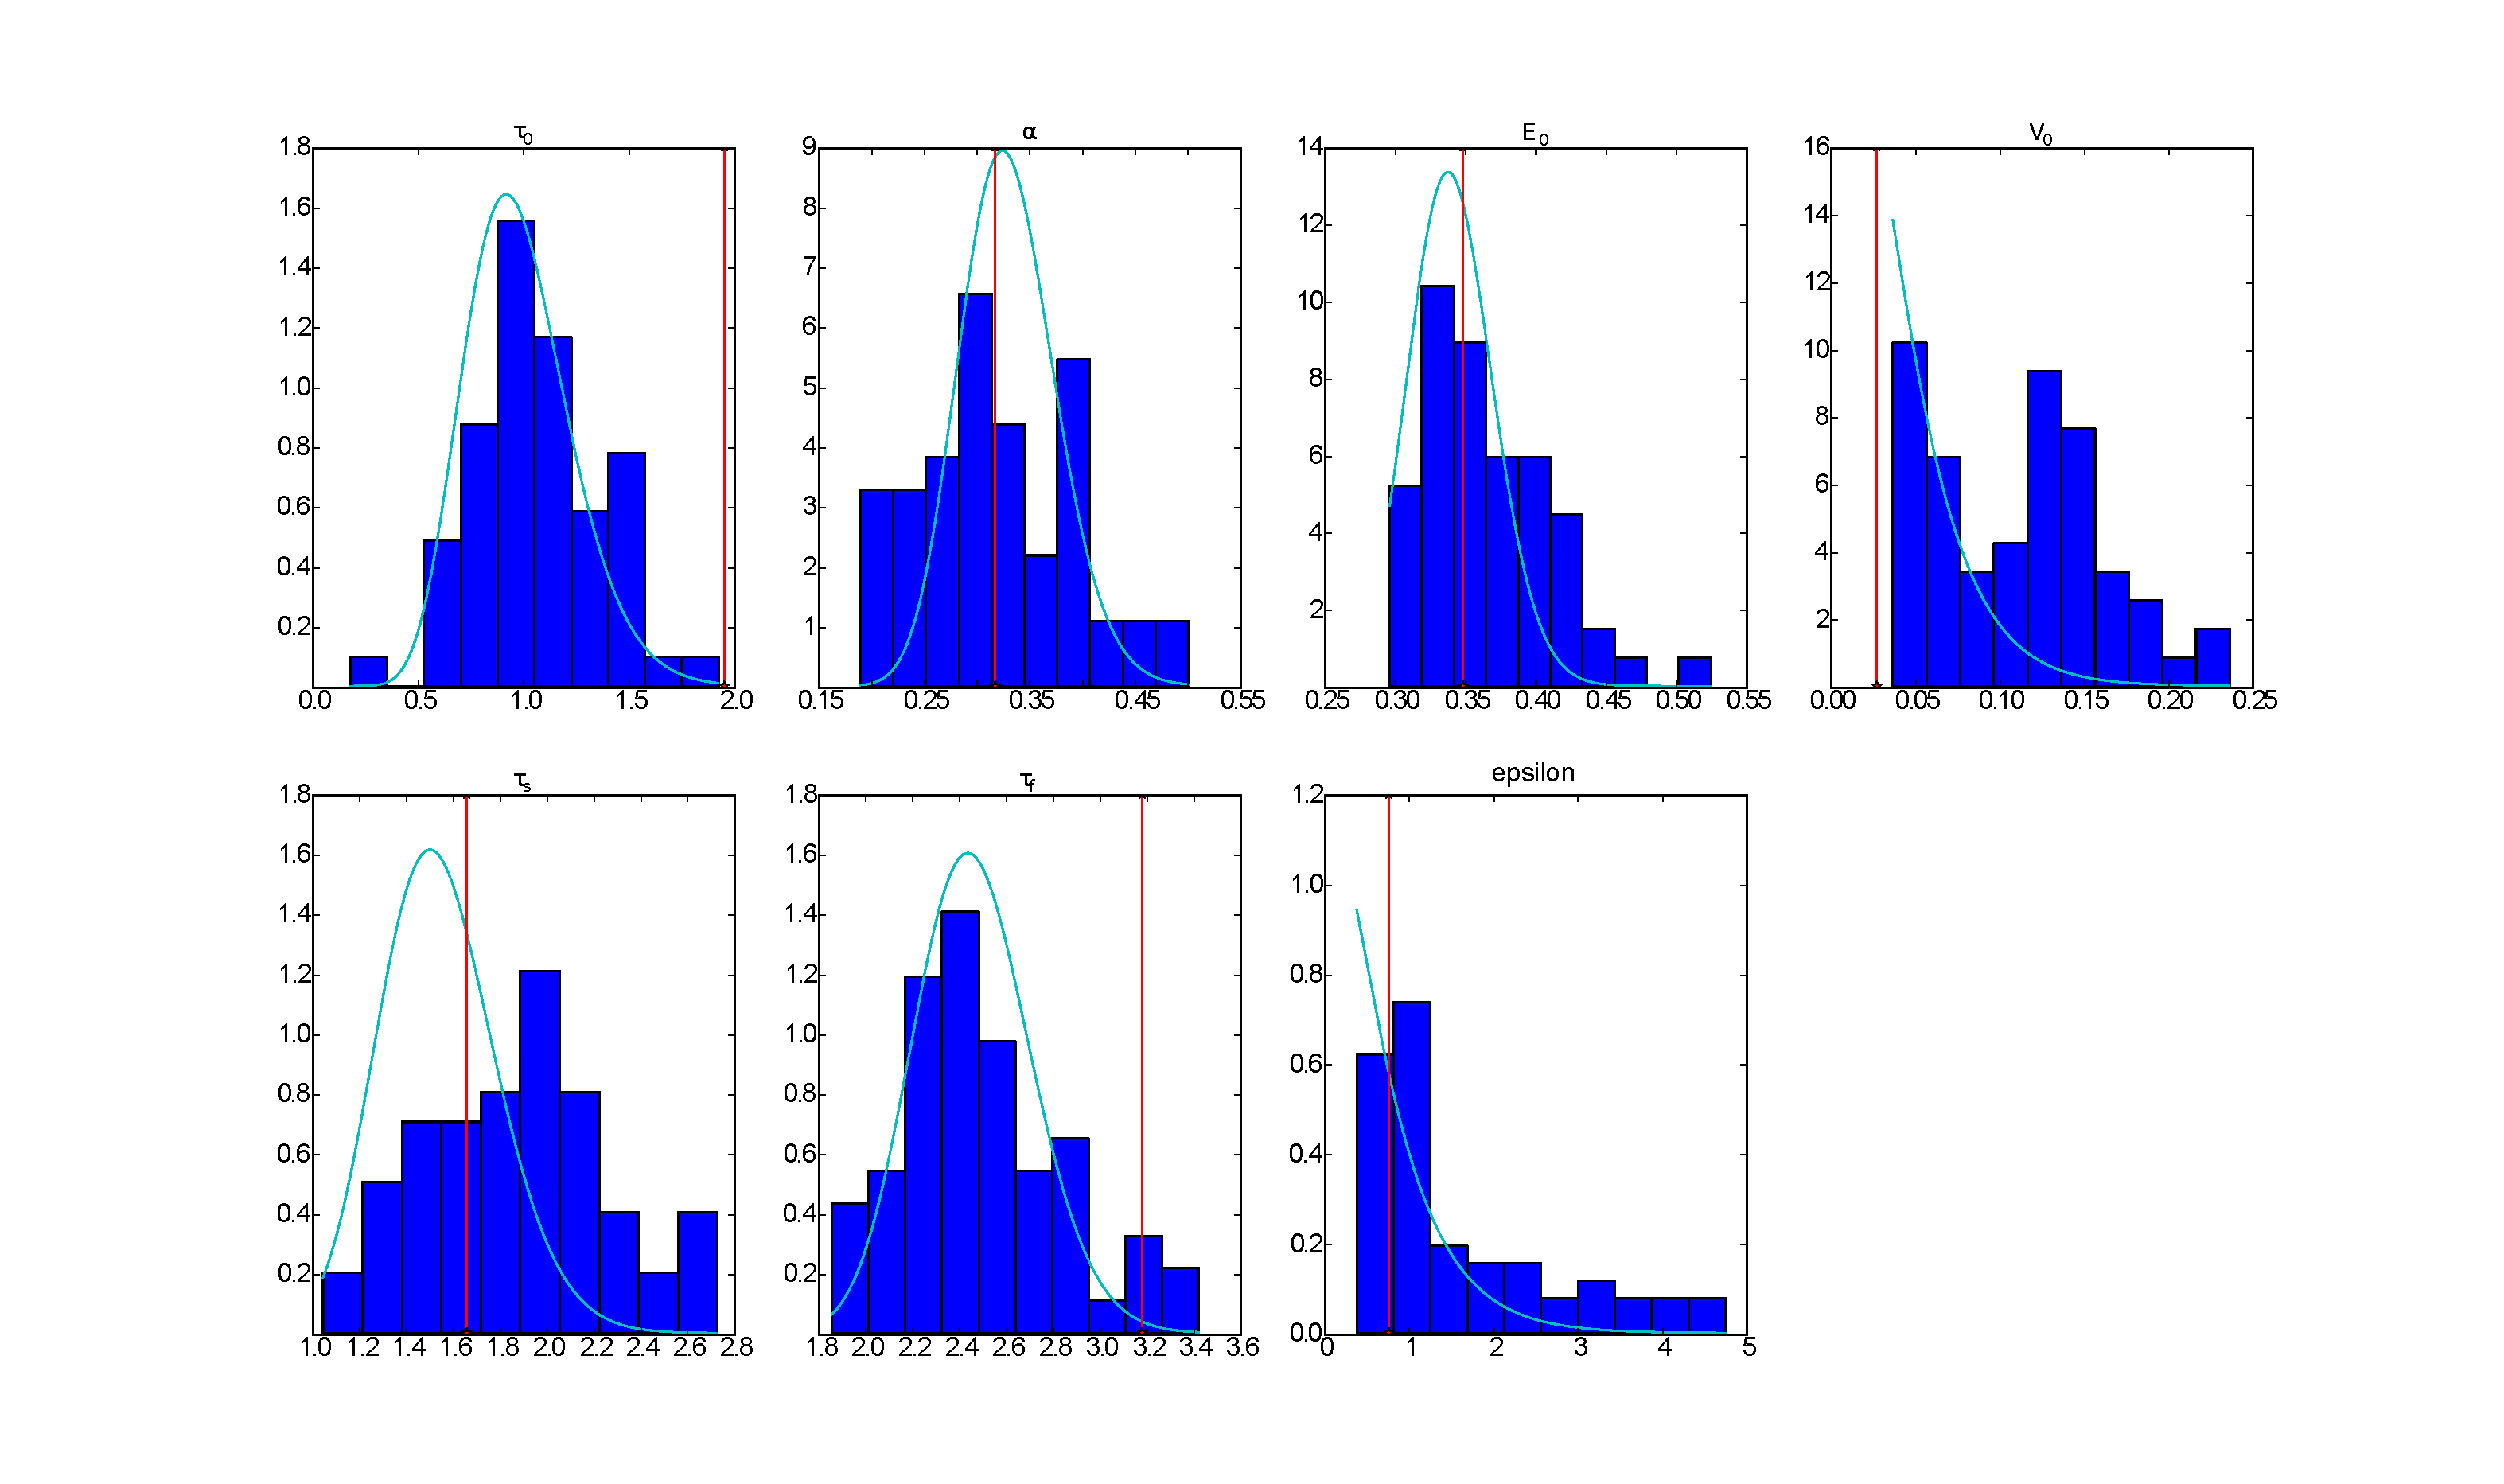
\includegraphics[clip=true,trim=5cm 2cm 5cm 2cm, width=\textwidth]{sec2hist}
\note{Histogram of estimated parameters.}
\note{Average SNR: $0.97$}
\note{Mutual Information greater than $0.15$.}
\end{figure}
\end{frame}

\begin{frame}{SPM vs. Mutual Information Map}
\begin{columns}
\begin{column}{.5\textwidth}
\begin{figure}
\setcounter{subfigure}{0}

\subfigure[SPM Results]{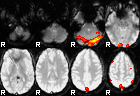
\includegraphics[width=.9\textwidth]{spm_hm}}
\subfigure{\includegraphics[width=.07\textwidth]{scale1}}
\note{SPM results. Units of activation are in Student's $t$-scores; higher 
        indicates higher assurance that the signal cannot have occurred 
        through noise alone.}
\label{fig:hm_canon_spm}
\end{figure}
\end{column}

\begin{column}{.5\textwidth}
\begin{figure}
\setcounter{subfigure}{1}
\subfigure[Particle Filter Results]{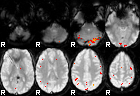
\includegraphics[width=.9\textwidth]{hm_mi_strict}}
\subfigure{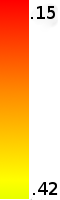
\includegraphics[height=1.5cm,width=.07\textwidth]{scale4}}
\note{Particle filter results. Units of activation are in mutual information;
    higher indicates more assured activation.}
\end{figure}
\end{column}
\end{columns}
\end{frame}

\begin{frame}{Particle Filter Results: Histogram}
\begin{figure}
\centering
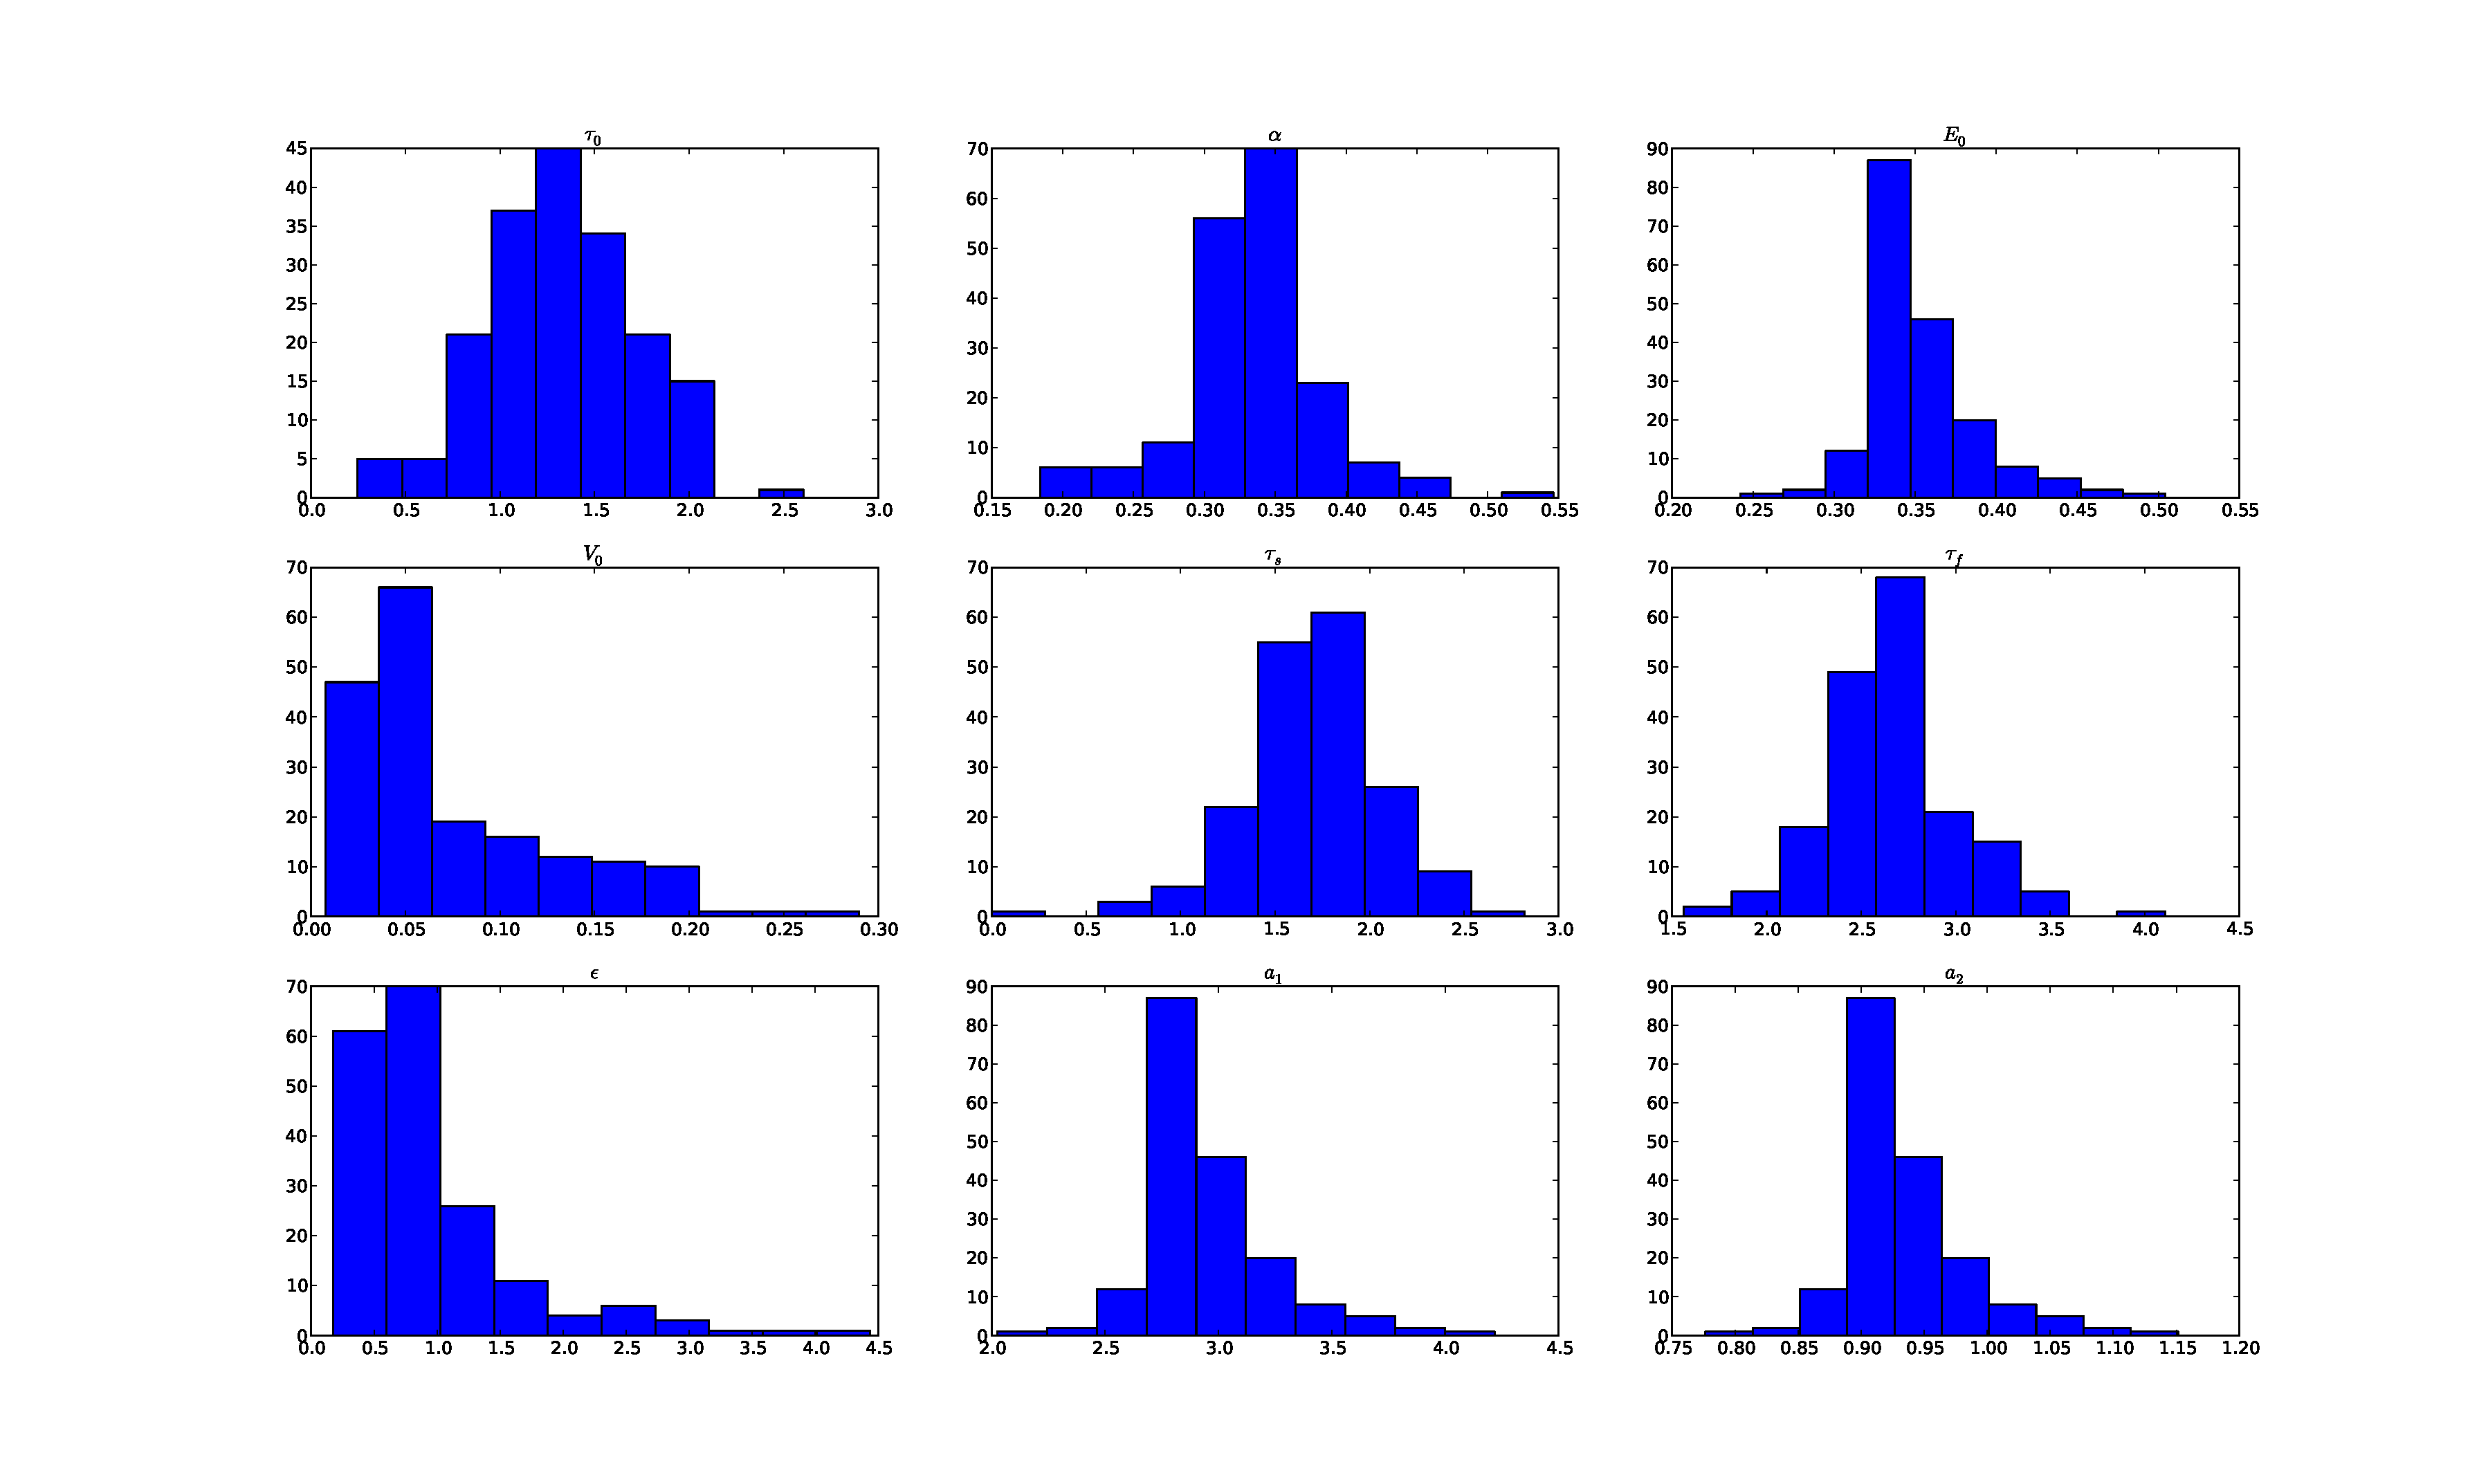
\includegraphics[clip=truew,trim=8cm 4cm 8cm 4cm,width=.8\textwidth]{realhist}
\note{Histogram of parameters in active regions ($M.I. > .15$).}
\end{figure}
\end{frame}

\section{Conclusion}
\begin{frame}{Factors Affecting Convergence}
    \begin{itemize}
        \item Weighting function
            \begin{itemize}
                \item Continuous, Long Tailed, Zero-Mean 
                \item Too wide $\rightarrow$ under-sensitivity, 
                    slow or no convergence
                \item Too thin $\rightarrow$ reduces robustness 
                    to noise, particle deprivation
            \end{itemize}
        \item Resampling 
            \begin{itemize}
                \item Stratified Resampling can result in truncated tails 
                        on posterior
                \item Regularized Resampling can result in over smoothing and 
                        slow convergence
            \end{itemize}
        \item Number of particles
            \begin{itemize}
                \item More particles give higher fidelity posterior
            \end{itemize}
    \end{itemize}
\end{frame}

\begin{frame}{Conclusion}
\begin{itemize}
    \item Summary:
    \begin{itemize}
    \item BOLD Parameters Ill-Defined
    \item Particle Filter Capable of good parameter BOLD estimate with 1000 particles
    \item Mutual Information performs well as estimate of Quality
    \end{itemize}
    \item Future Works
    \begin{itemize}
        \item Further limitations should be placed on priors, Deneux 
            et al. \cite{Deneux2006} shows that parameters could imposed.
        \item Automation of Weighting Function
        \item Analysis of joint parameter distribution for populations
        \item Real Time analysis possible for multiple Voxels, similar to
            De Charms et al. \cite{DeCharms2005}

    \end{itemize}
\end{itemize}
\end{frame}

\begin{frame}{Questions?}
\end{frame}

%% All of the following is optional and typically not needed. 
%\appendix
%\section<presentation>*{\appendixname}
%\subsection<presentation>*{For Further Reading}

\begin{frame}[allowframebreaks]
  \bibliographystyle{plain}
  \bibliography{../library}
\end{frame}

\appendix
\begin{frame}{SPM vs. Mutual Information Map, SPM}
\begin{figure}
\setcounter{subfigure}{0}
\subfigure[SPM Results]{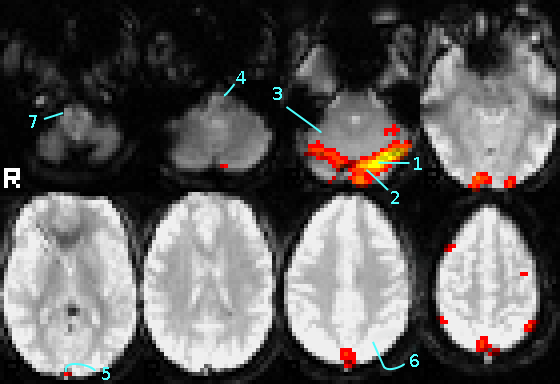
\includegraphics[width=.8\textwidth]{images/spm_hm}}
\subfigure{\includegraphics[scale=.5]{images/scale1}}
\note{SPM results. Units of activation are in Student's $t$-scores; higher 
        indicates higher assurance that the signal cannot have occurred 
        through noise alone.}
\end{figure}
\end{frame}

\begin{frame}{SPM vs. Mutual Information Map, $M.I. > .15$}
\begin{figure}
\setcounter{subfigure}{1}
\subfigure[Particle Filter Results]{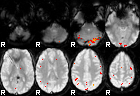
\includegraphics[width=.8\textwidth]{hm_mi_strict}}
\subfigure{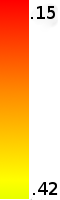
\includegraphics[width=.1\textwidth]{scale4}}
\note{Particle filter results. Units of activation are in mutual information;
    higher indicates more assured activation.}
\end{figure}
\end{frame}

\begin{frame}{SPM vs. Mutual Information Map, $M.I. > .1$}
\begin{figure}
\setcounter{subfigure}{2}
\subfigure[Particle Filter Results]{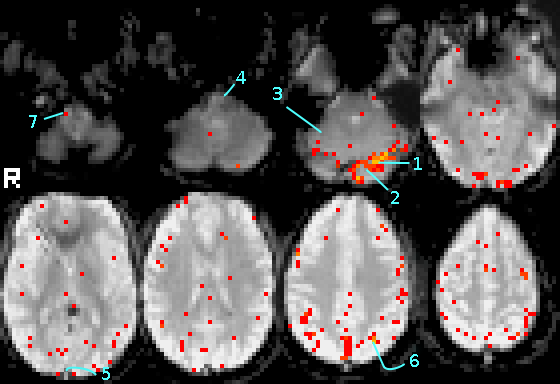
\includegraphics[width=.8\textwidth]{mi_hm}}
\subfigure{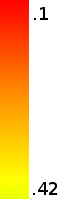
\includegraphics[width=.1\textwidth]{scale6}}
\note{Particle filter results. Units of activation are in mutual information;
    higher indicates more assured activation.}
\end{figure}
\end{frame}

\begin{frame}{1: 37-14-7}
\setcounter{subfigure}{0}
\begin{figure}
\centering
\subfigure[Particle Filter]{\label{fig:comp1pfilter} 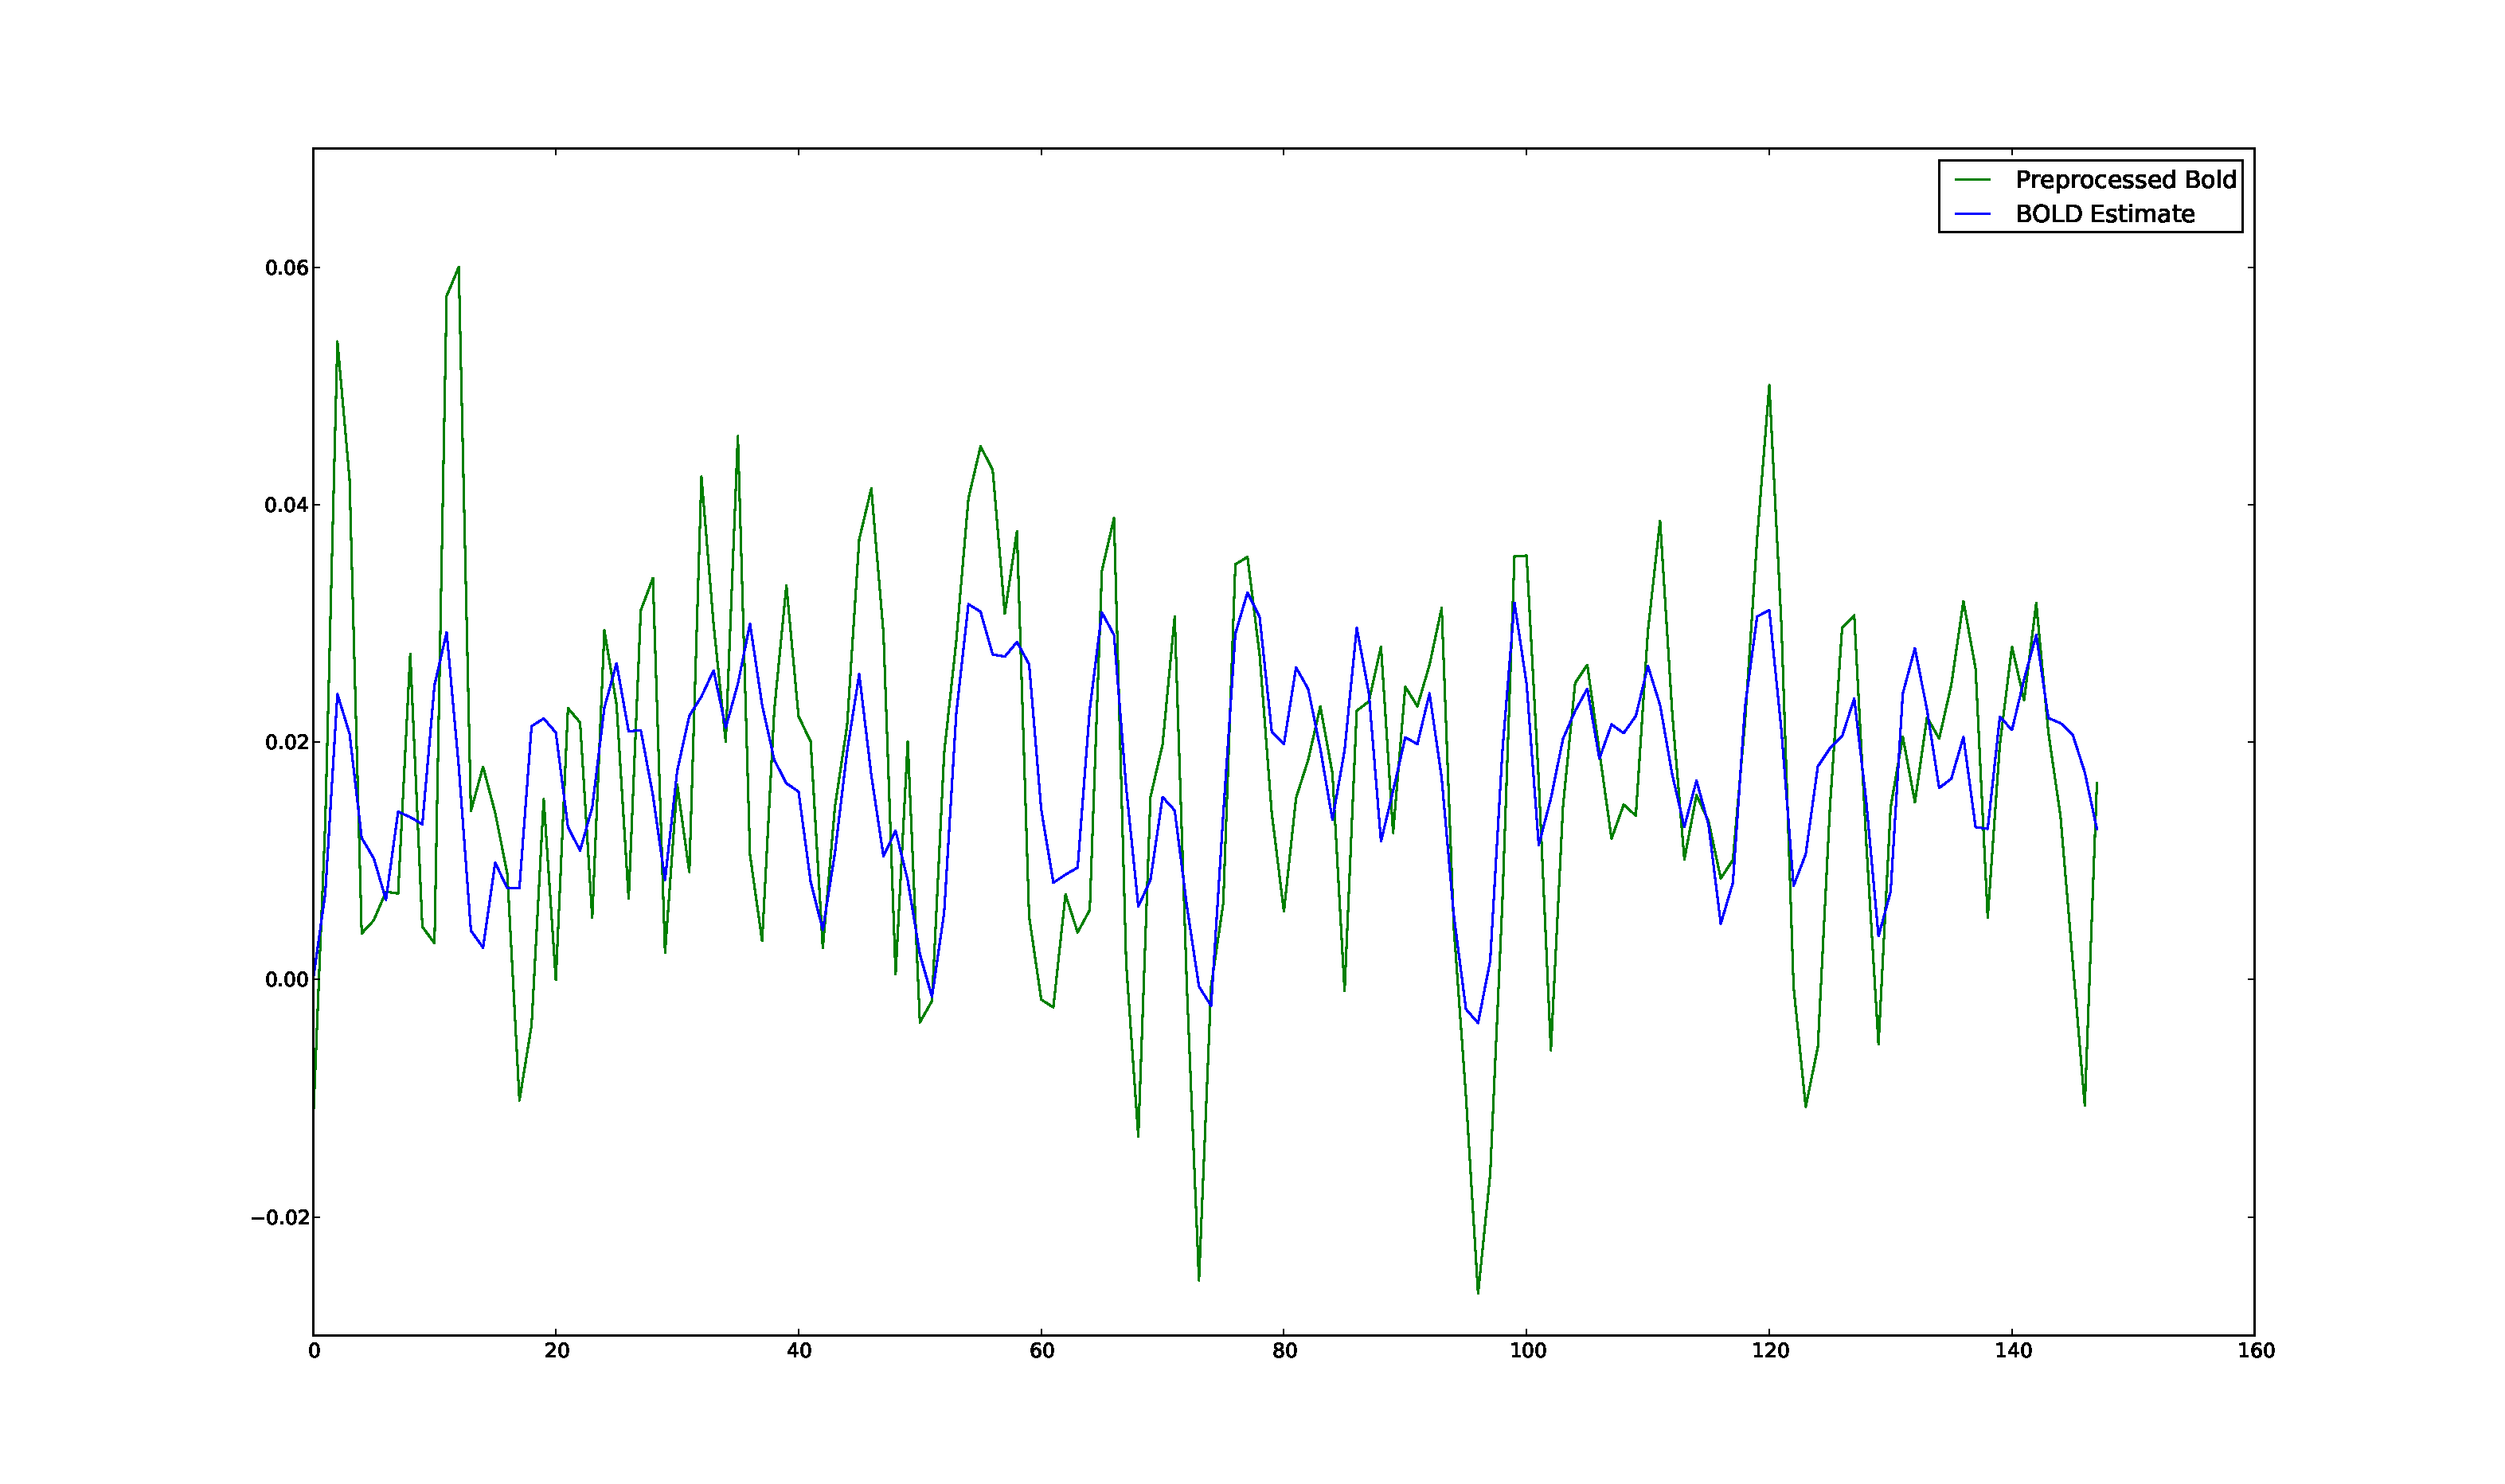
\includegraphics[clip=true,trim=5cm 1cm 4cm 1cm,width=.4\textwidth]{images/1_pfilter_37_14_7}}
\subfigure[SPM]{\label{fig:comp1spm} 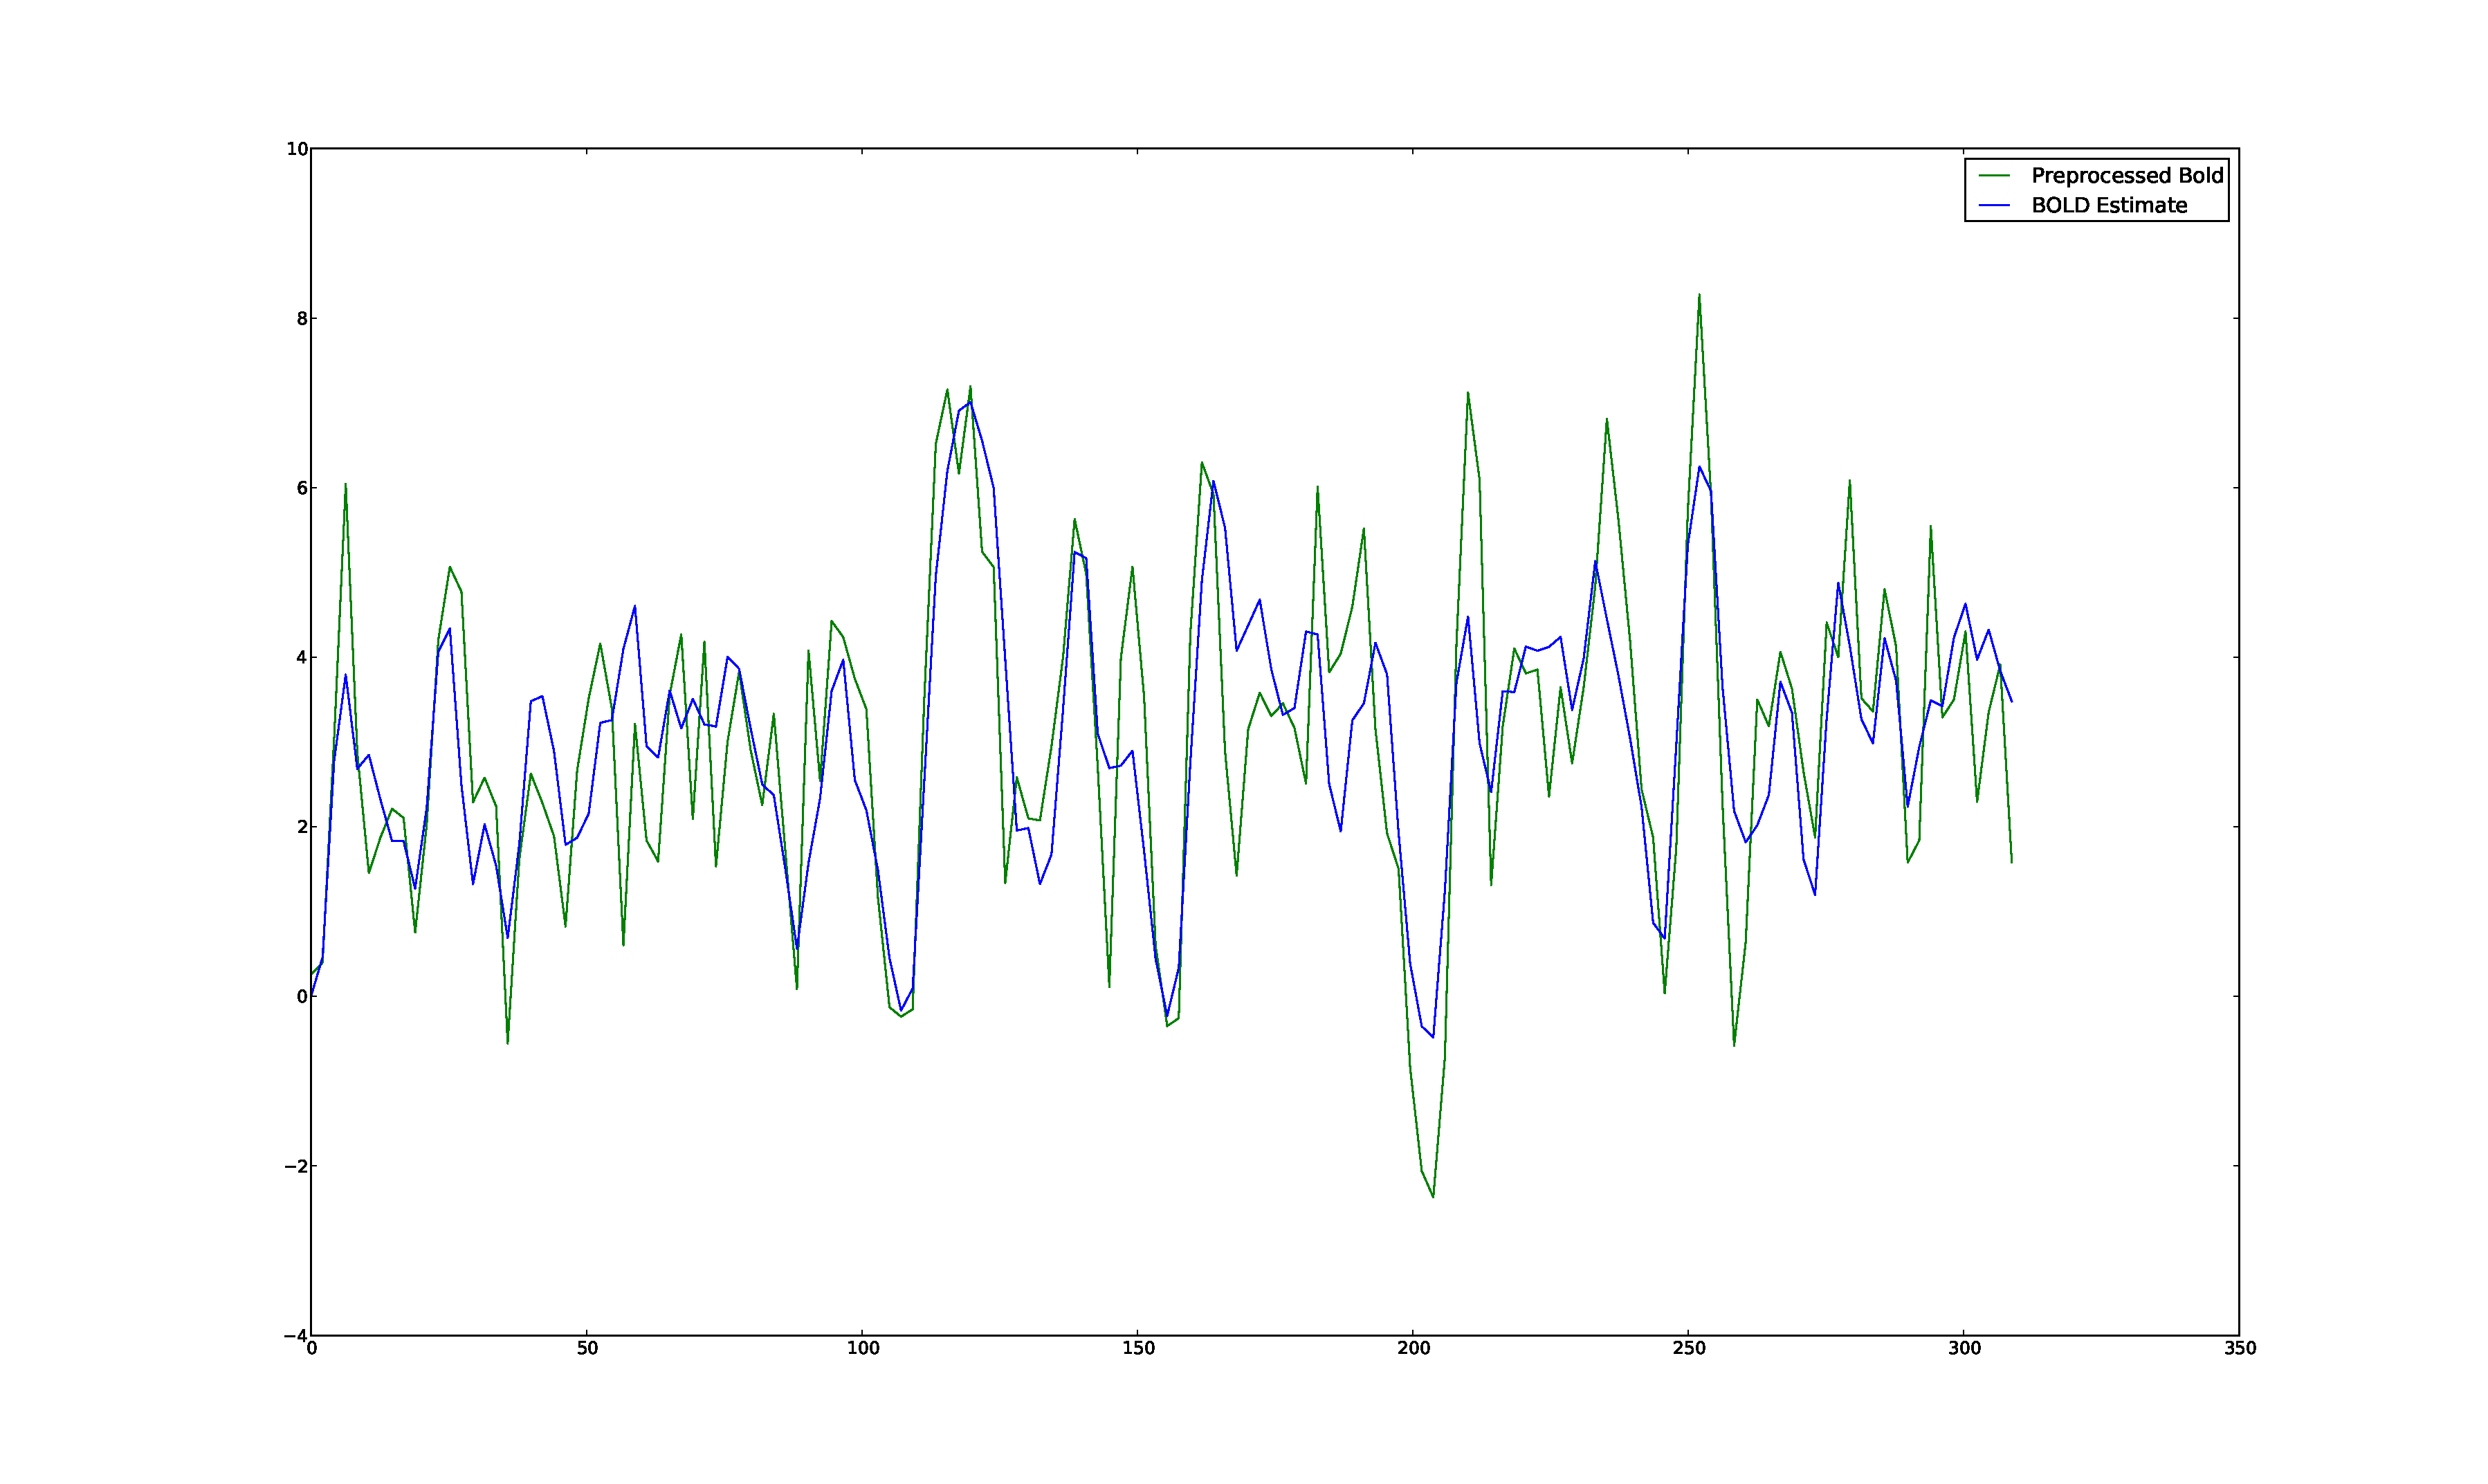
\includegraphics[clip=true,trim=5cm 1cm 4cm 1cm,width=.4\textwidth]{images/1_spm_37_14_7}}
\caption{Section 1, Estimated vs. Actual BOLD response. $t$-Score: $10.71$, Mutual Information: $0.33$, Residual: $0.72$.}
\label{fig:comp1}
\end{figure}
\end{frame}

\begin{frame}{2: 34-12-7}
\setcounter{subfigure}{0}
\begin{figure}
\centering
\subfigure[Particle Filter]{\label{fig:comp2pfilter} 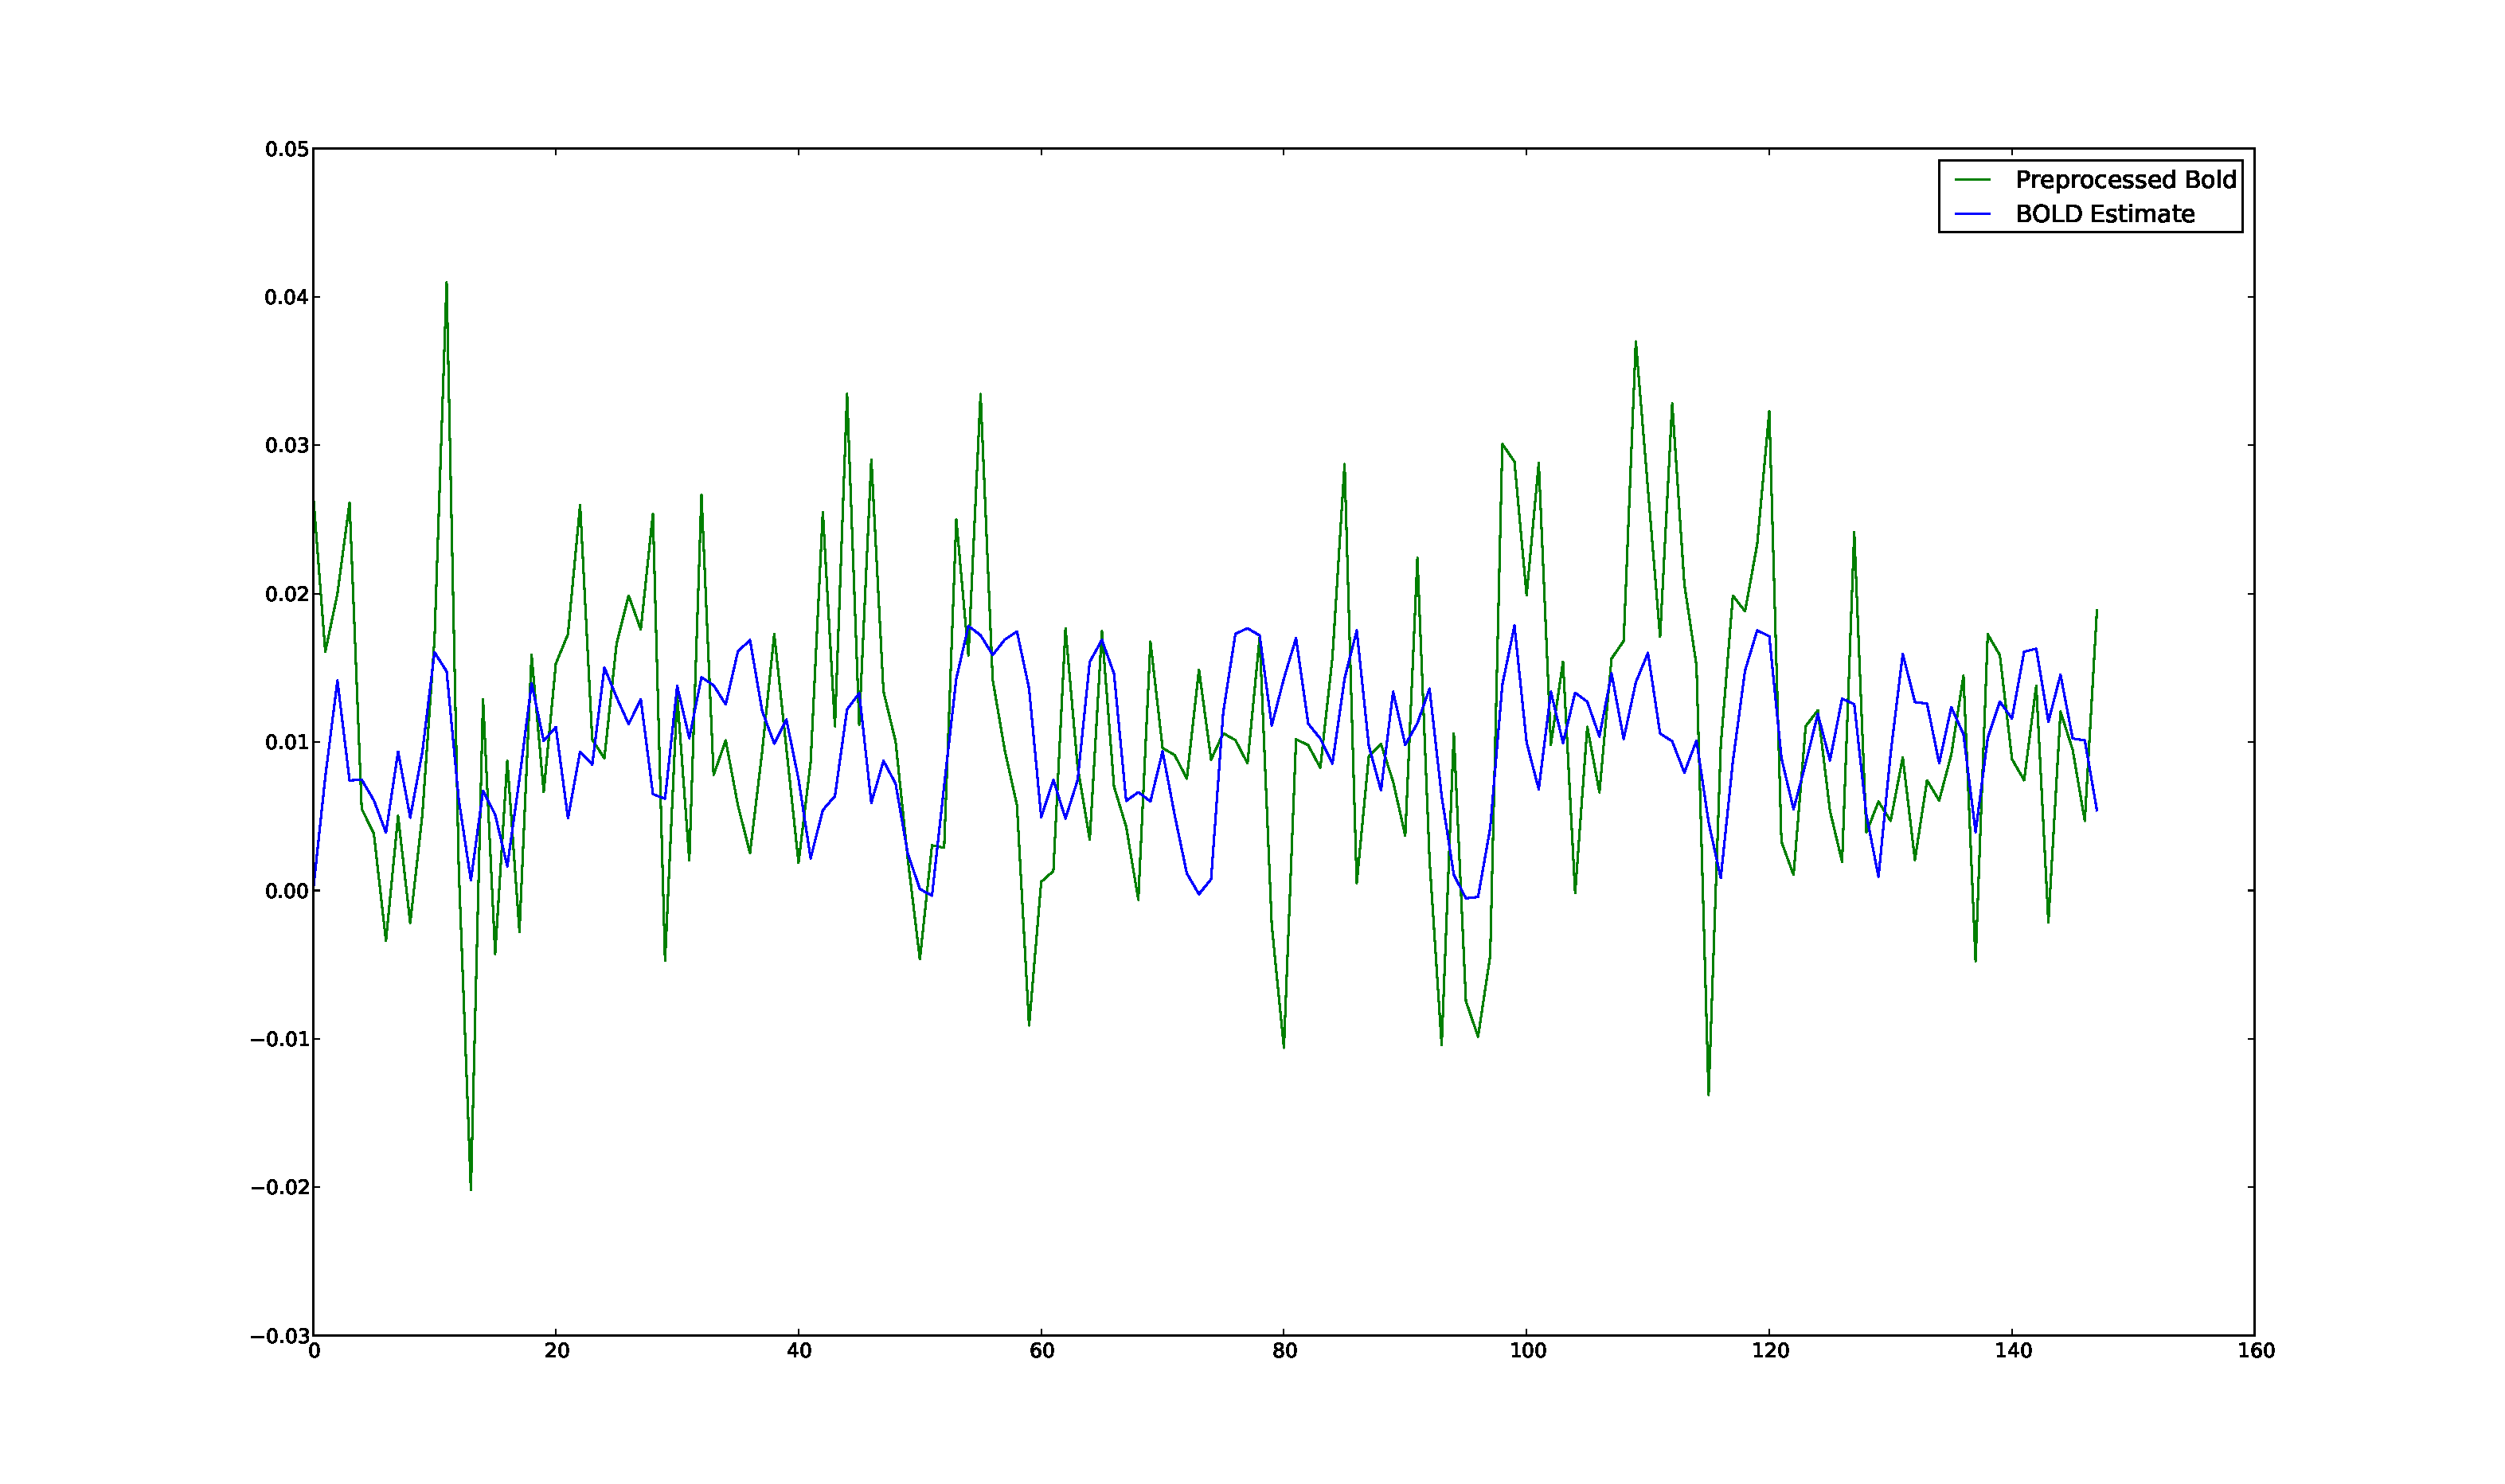
\includegraphics[clip=true,trim=5cm 1cm 4cm 1cm,width=.4\textwidth]{images/2_pfilter_34_12_7}}
\subfigure[SPM]{\label{fig:comp2spm} 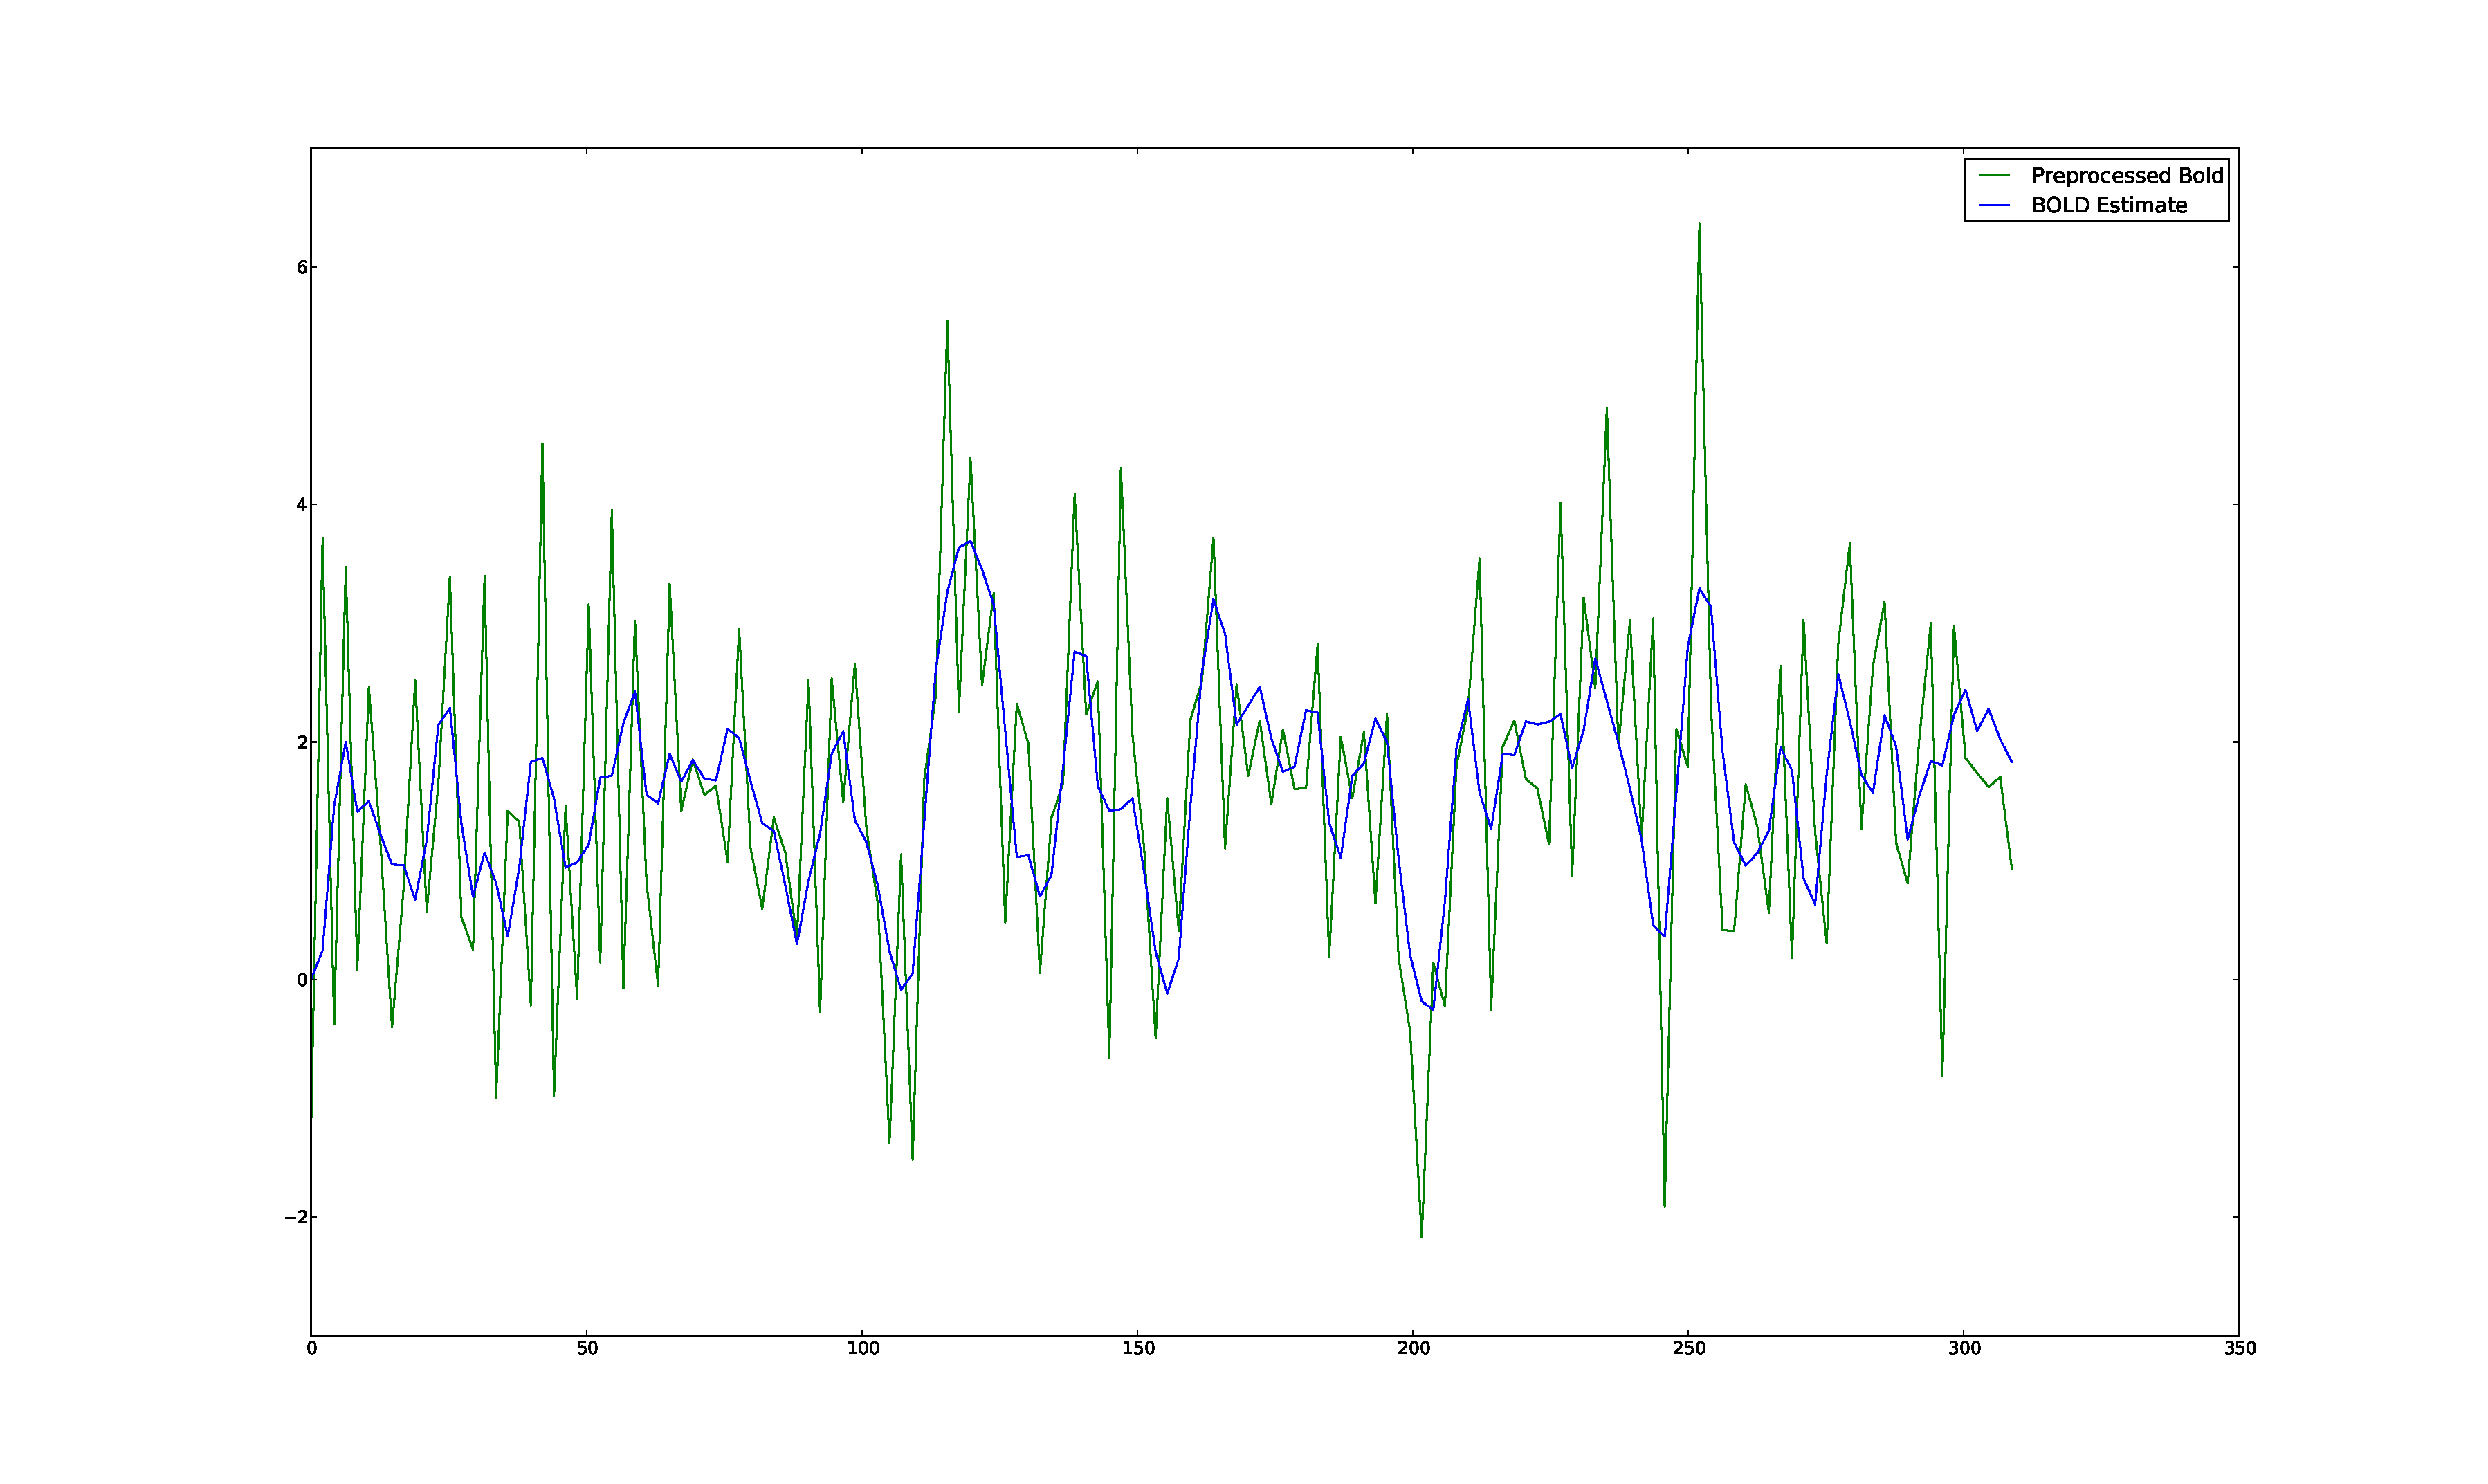
\includegraphics[clip=true,trim=5cm 1cm 4cm 1cm,width=.4\textwidth]{images/2_spm_34_12_7}}
\caption{Section 2, Estimated vs. Actual BOLD response. $t$-Score: $6.97$, Mutual Information: $0.04$, Residual: $1.02$.}
\label{fig:comp2}
\end{figure}
\end{frame}

\begin{frame}{3: 23-21-7}
\setcounter{subfigure}{0}
\begin{figure}
\centering
\subfigure[Particle Filter]{\label{fig:comp3pfilter} 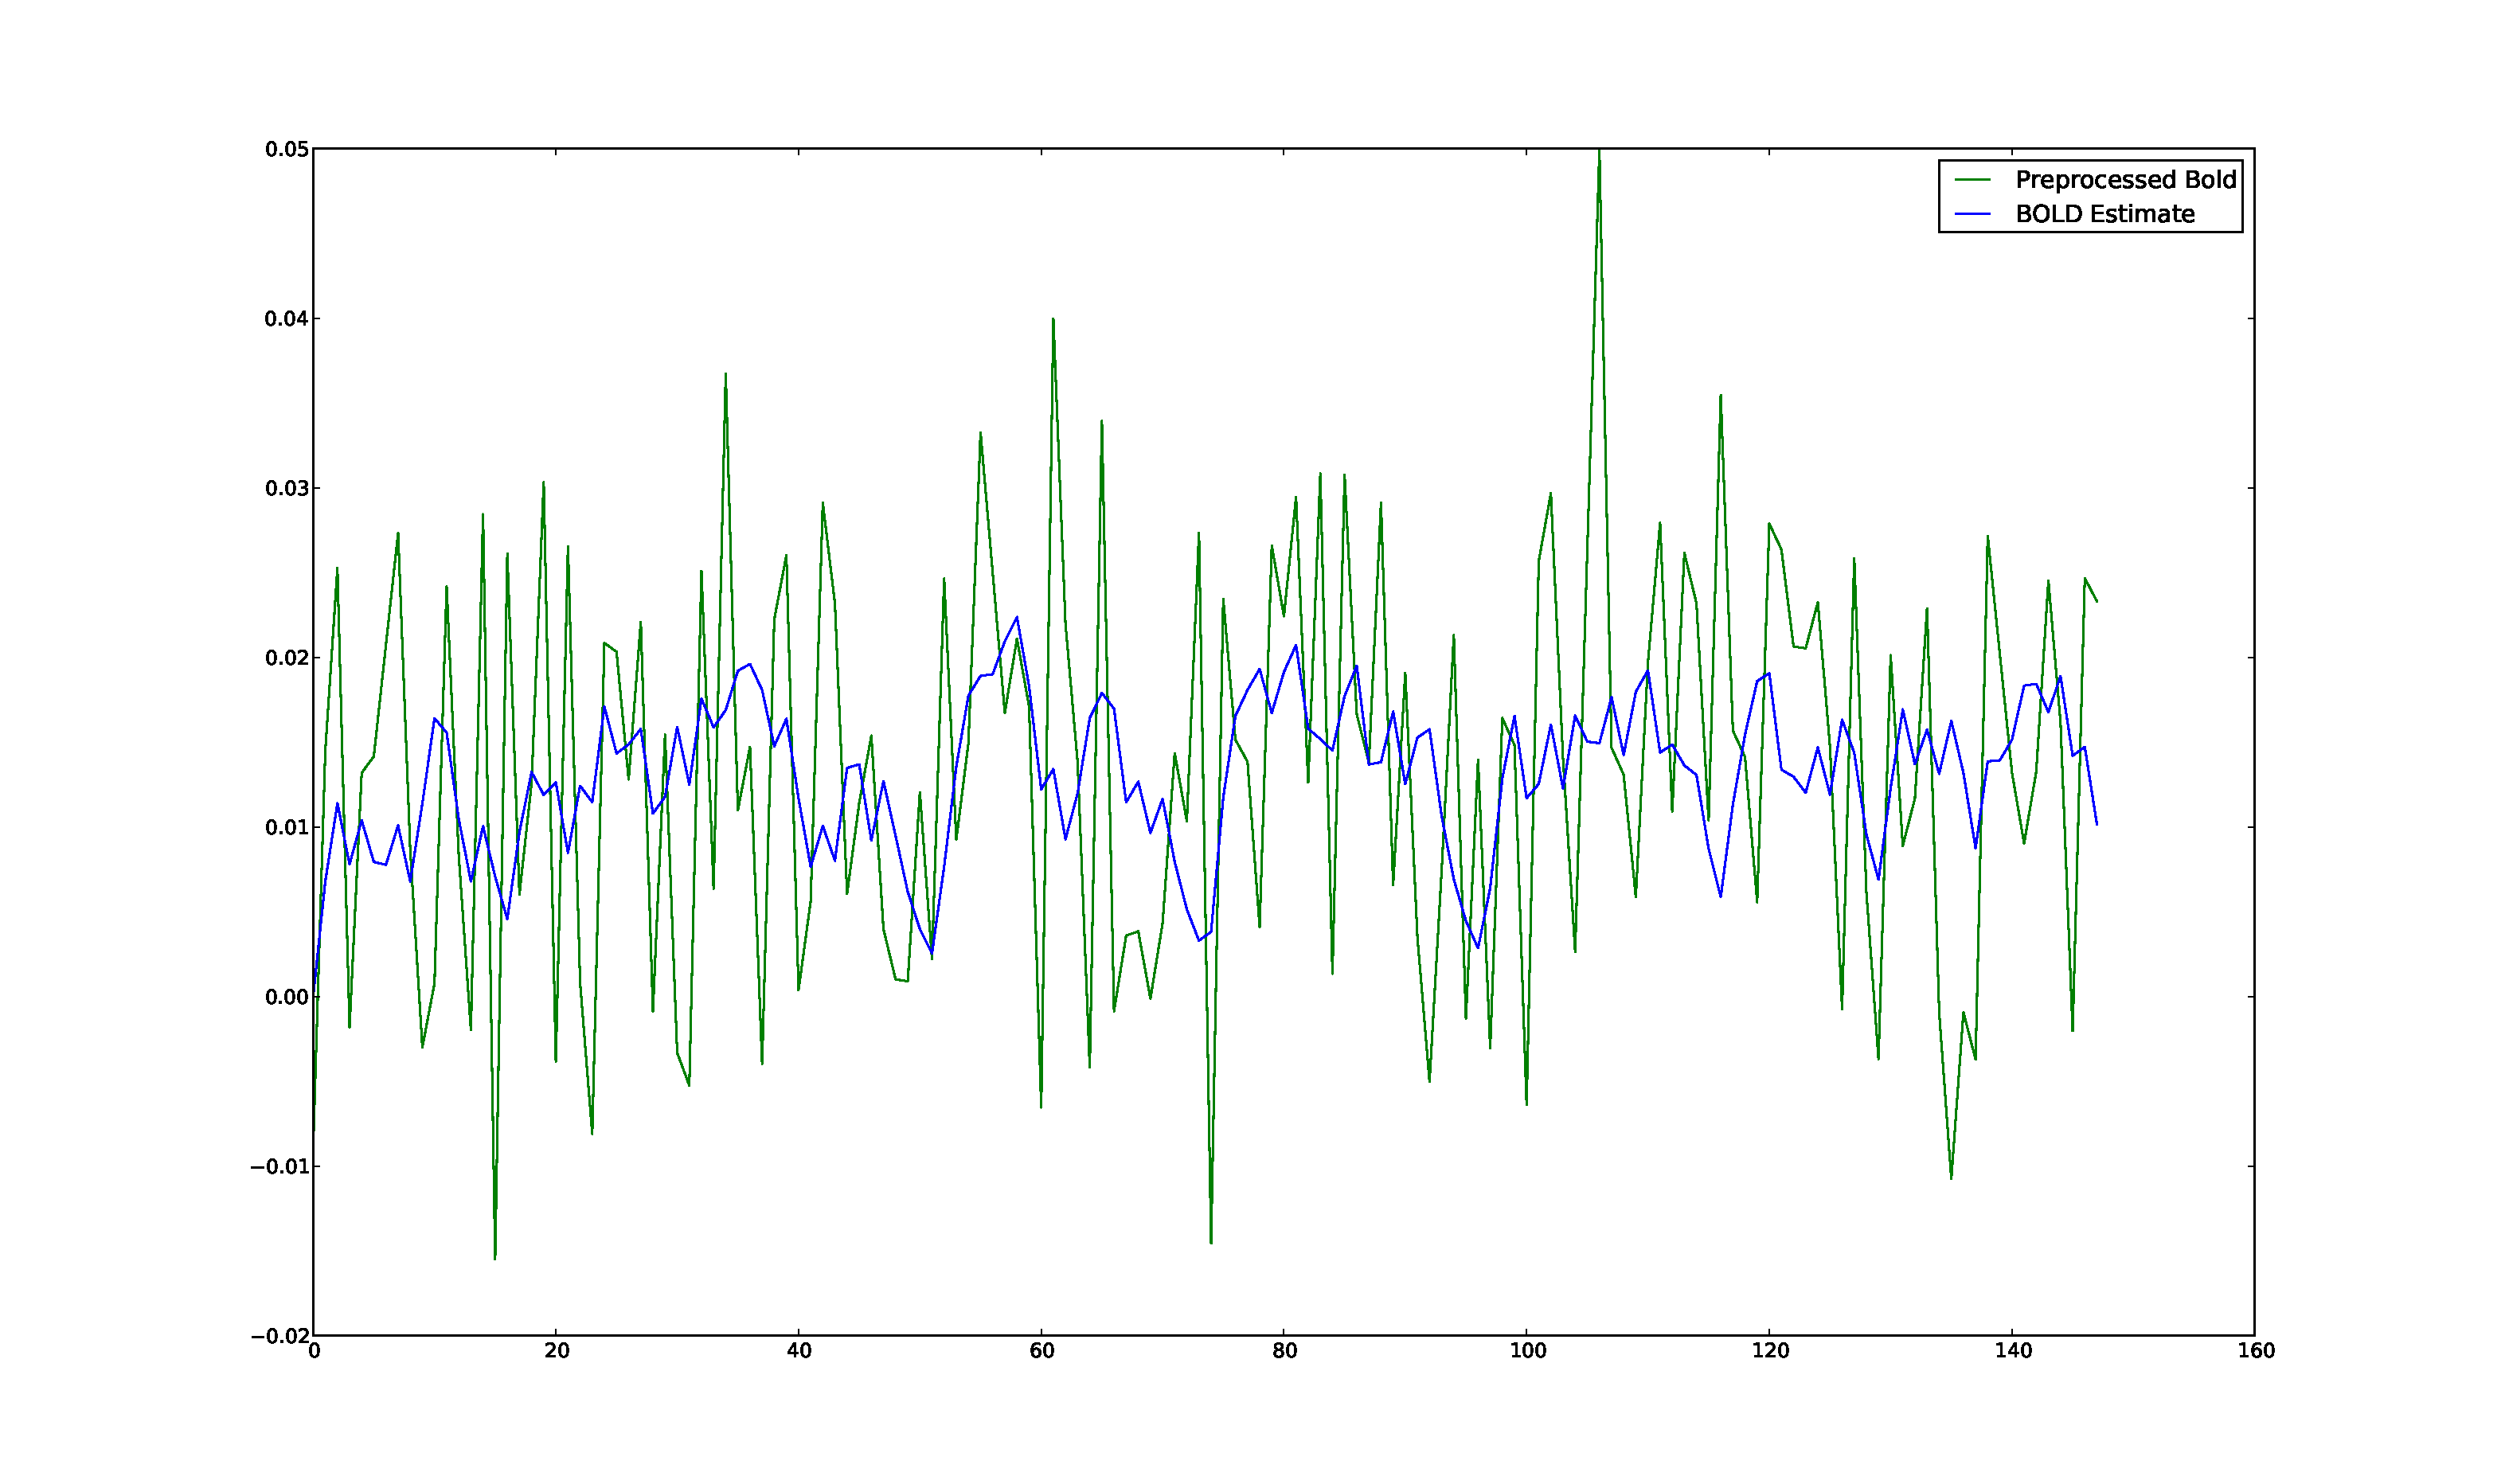
\includegraphics[clip=true,trim=5cm 1cm 4cm 1cm,width=.4\textwidth]{images/3_pfilter_23_21_7}}
\subfigure[SPM]{\label{fig:comp3spm} 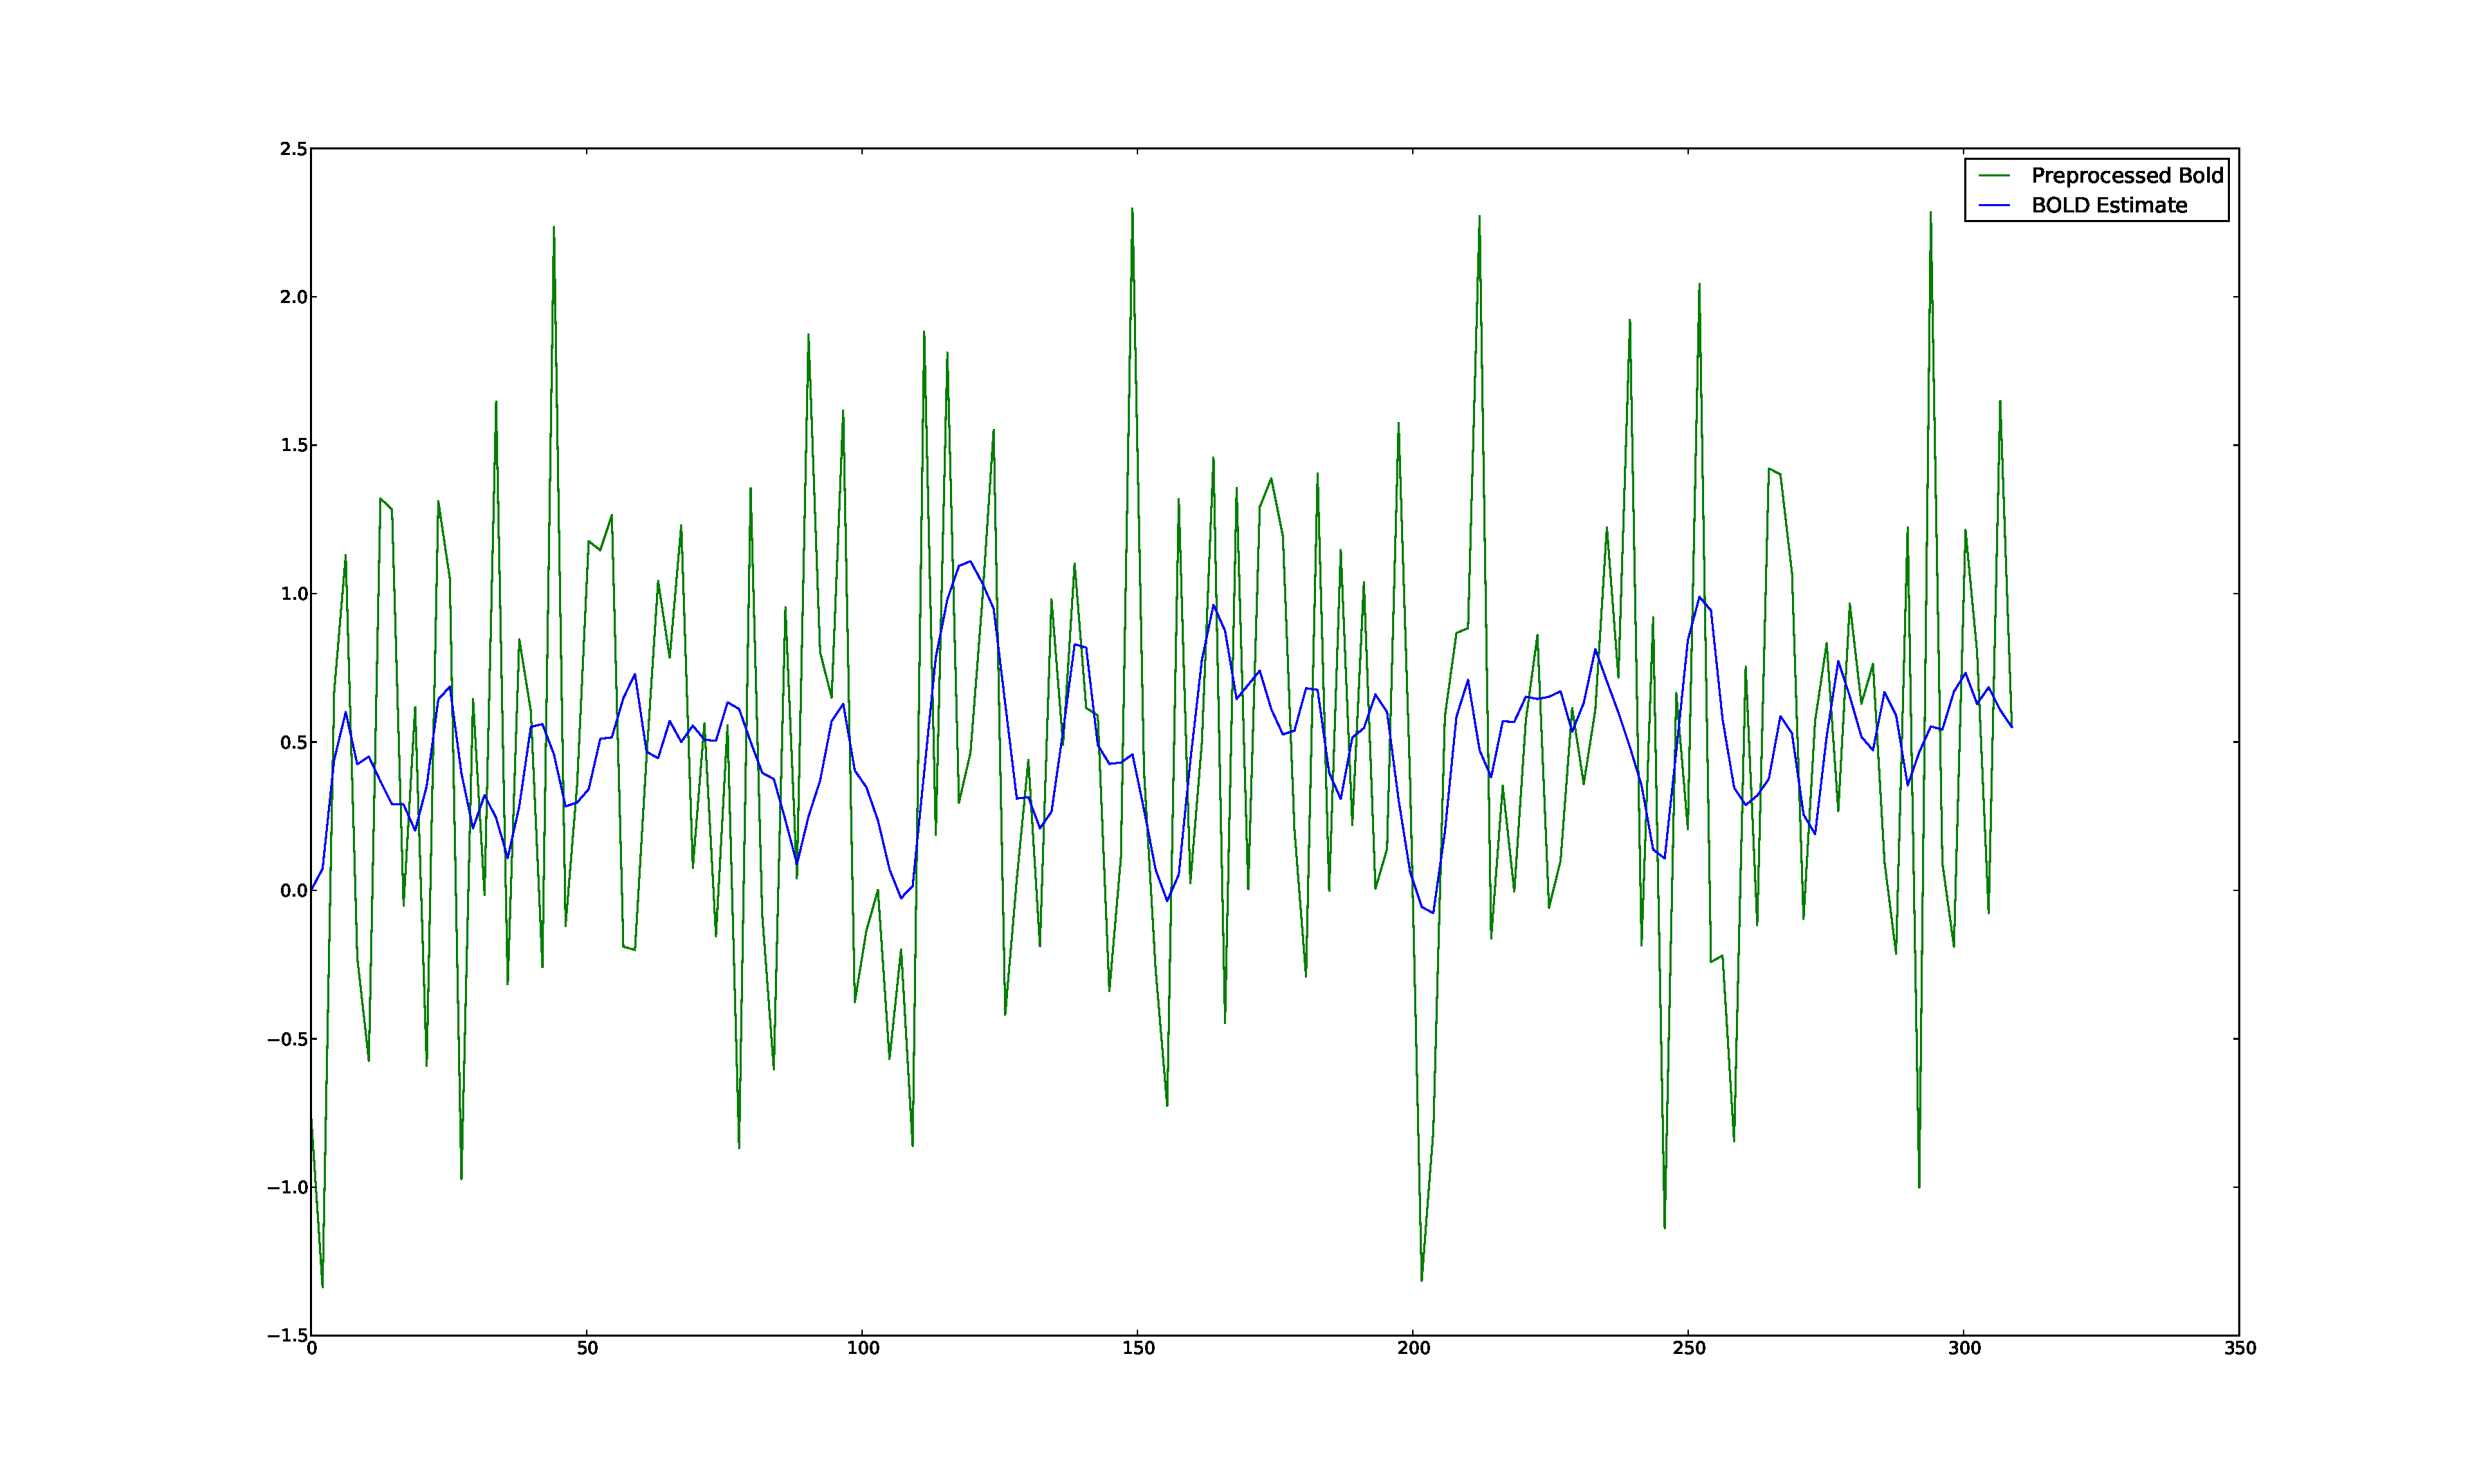
\includegraphics[clip=true,trim=5cm 1cm 4cm 1cm,width=.4\textwidth]{images/3_spm_23_21_7}}
\caption{Section 3, Estimated vs. Actual BOLD response. $t$-Score: $2.85$, Mutual Information: $-0.03$, Residual: $0.81$.}
\label{fig:comp3}
\end{figure}
\end{frame}

\begin{frame}{4: 33-40-4}
\setcounter{subfigure}{0}
\begin{figure}
\centering
\subfigure[Particle Filter]{\label{fig:comp4pfilter} 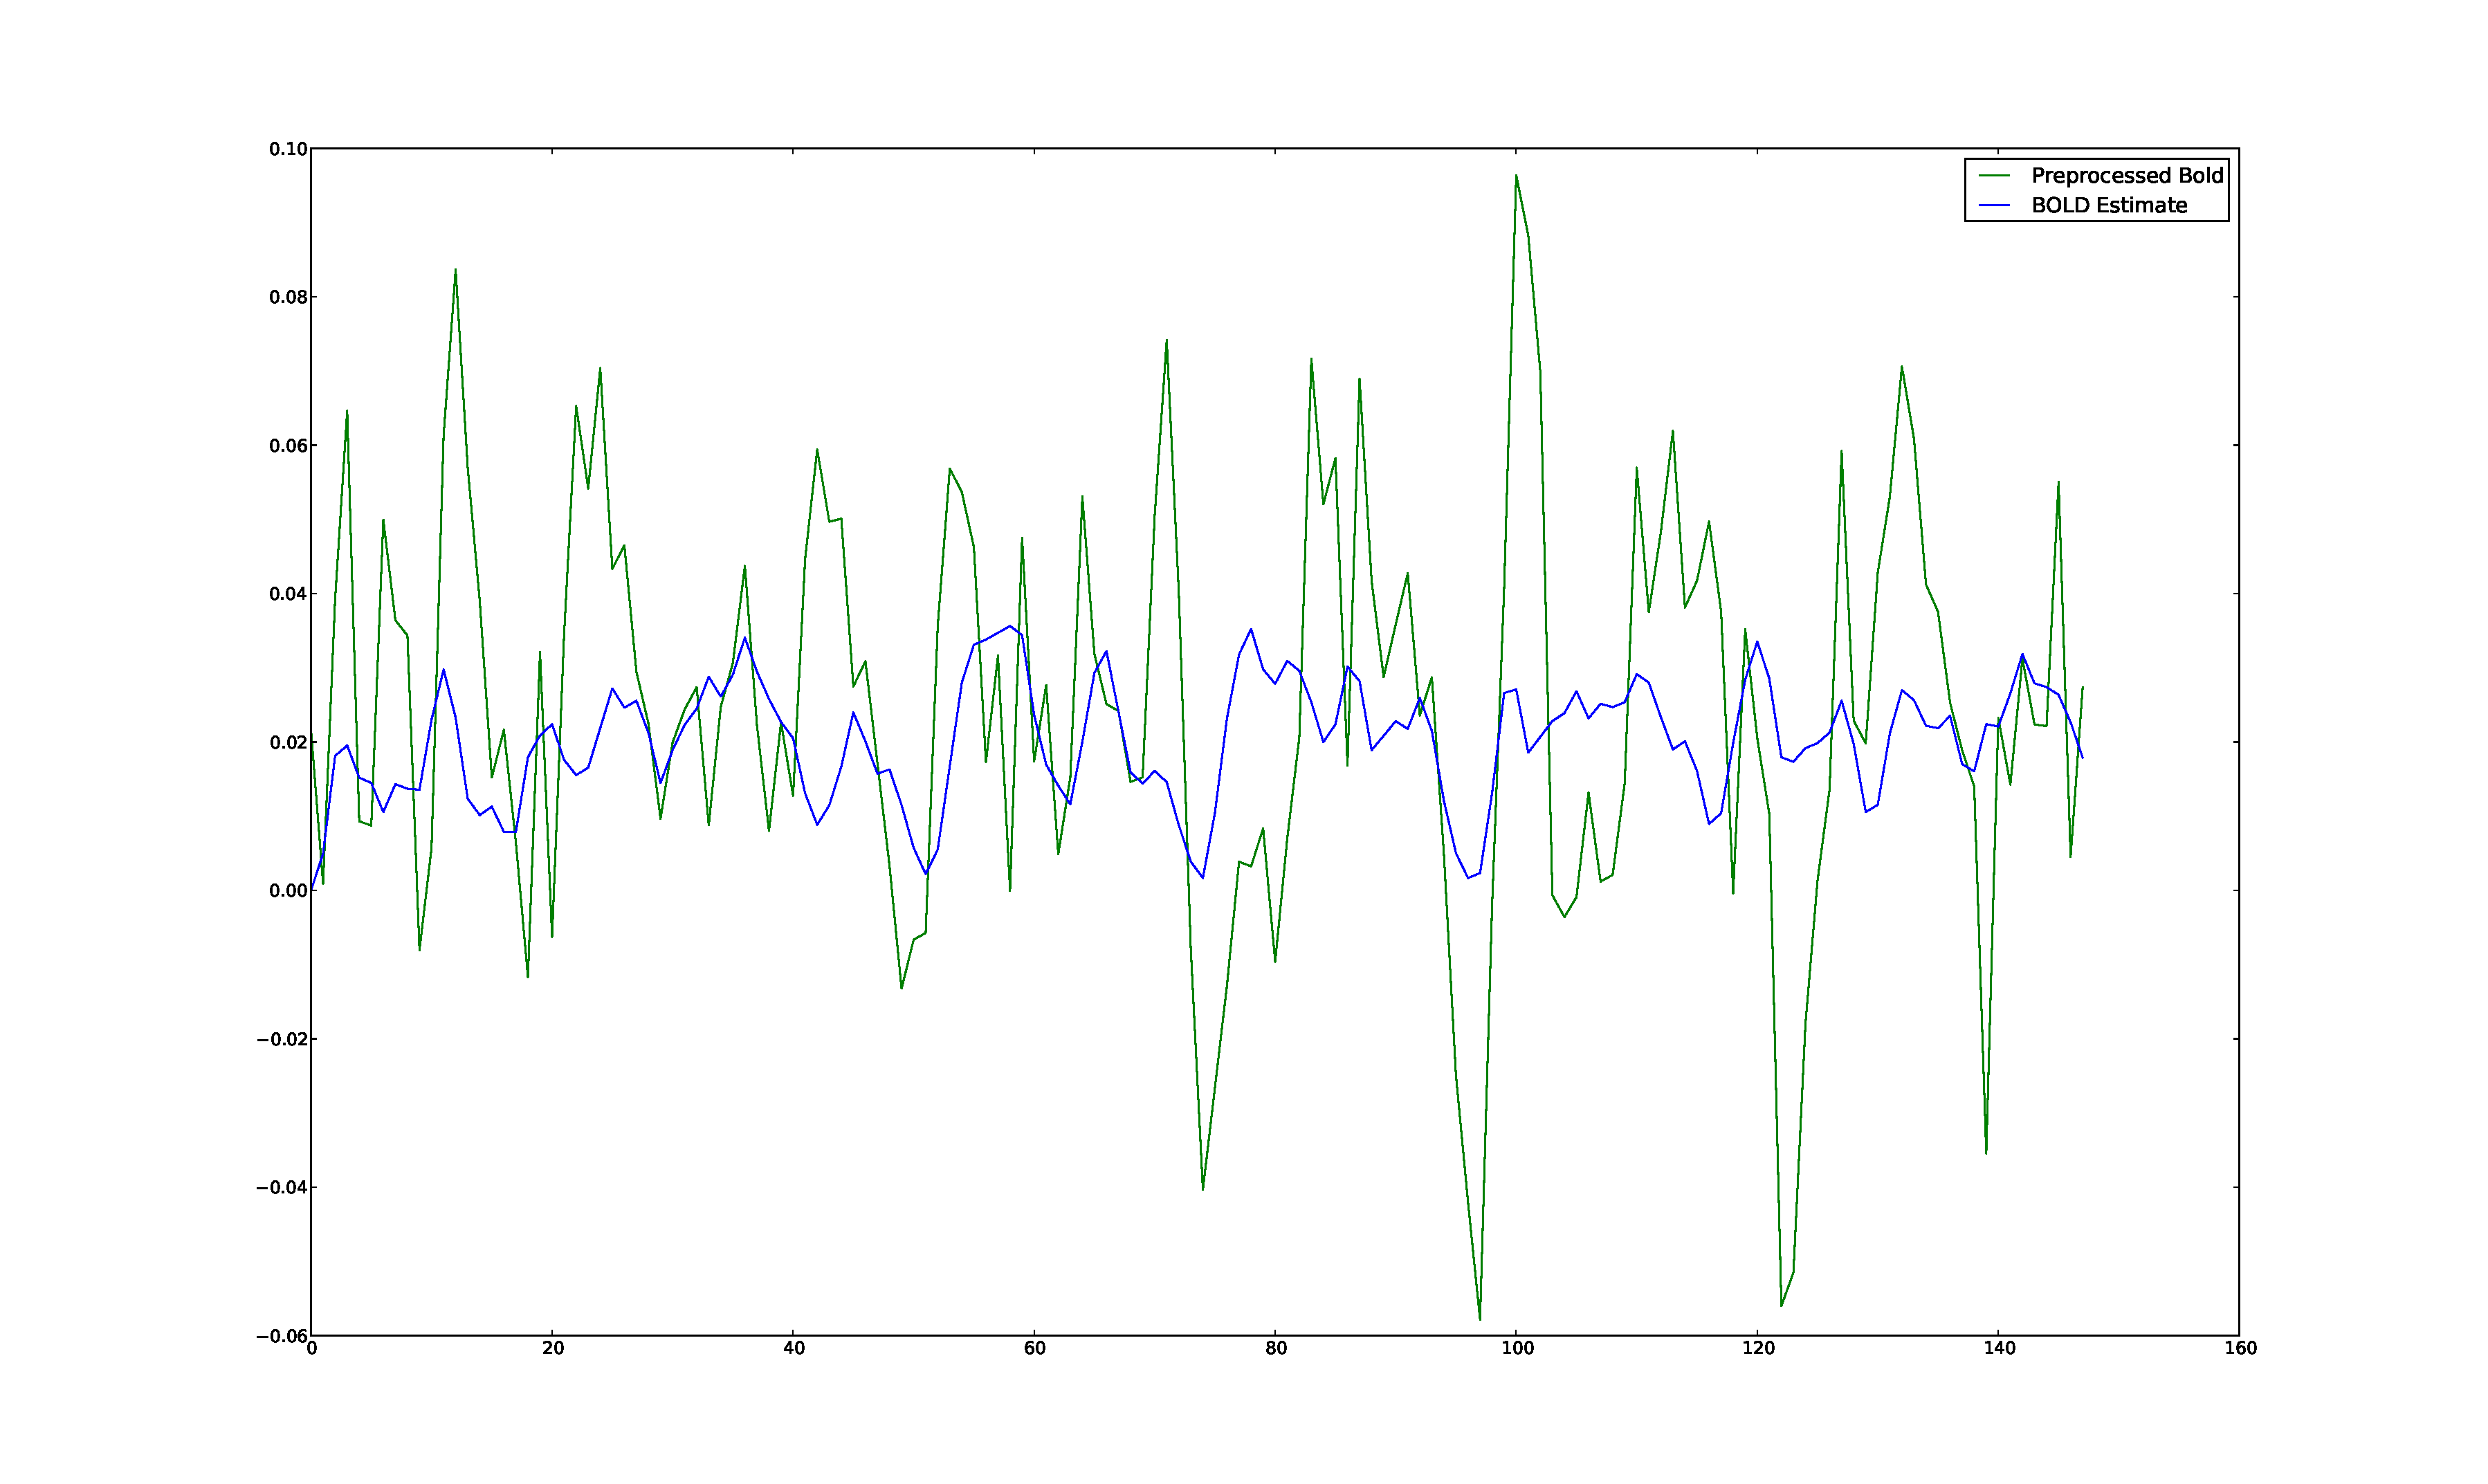
\includegraphics[clip=true,trim=5cm 1cm 4cm 1cm,width=.4\textwidth]{images/4_pfilter_26_15_7}}
\subfigure[SPM]{\label{fig:comp4spm} 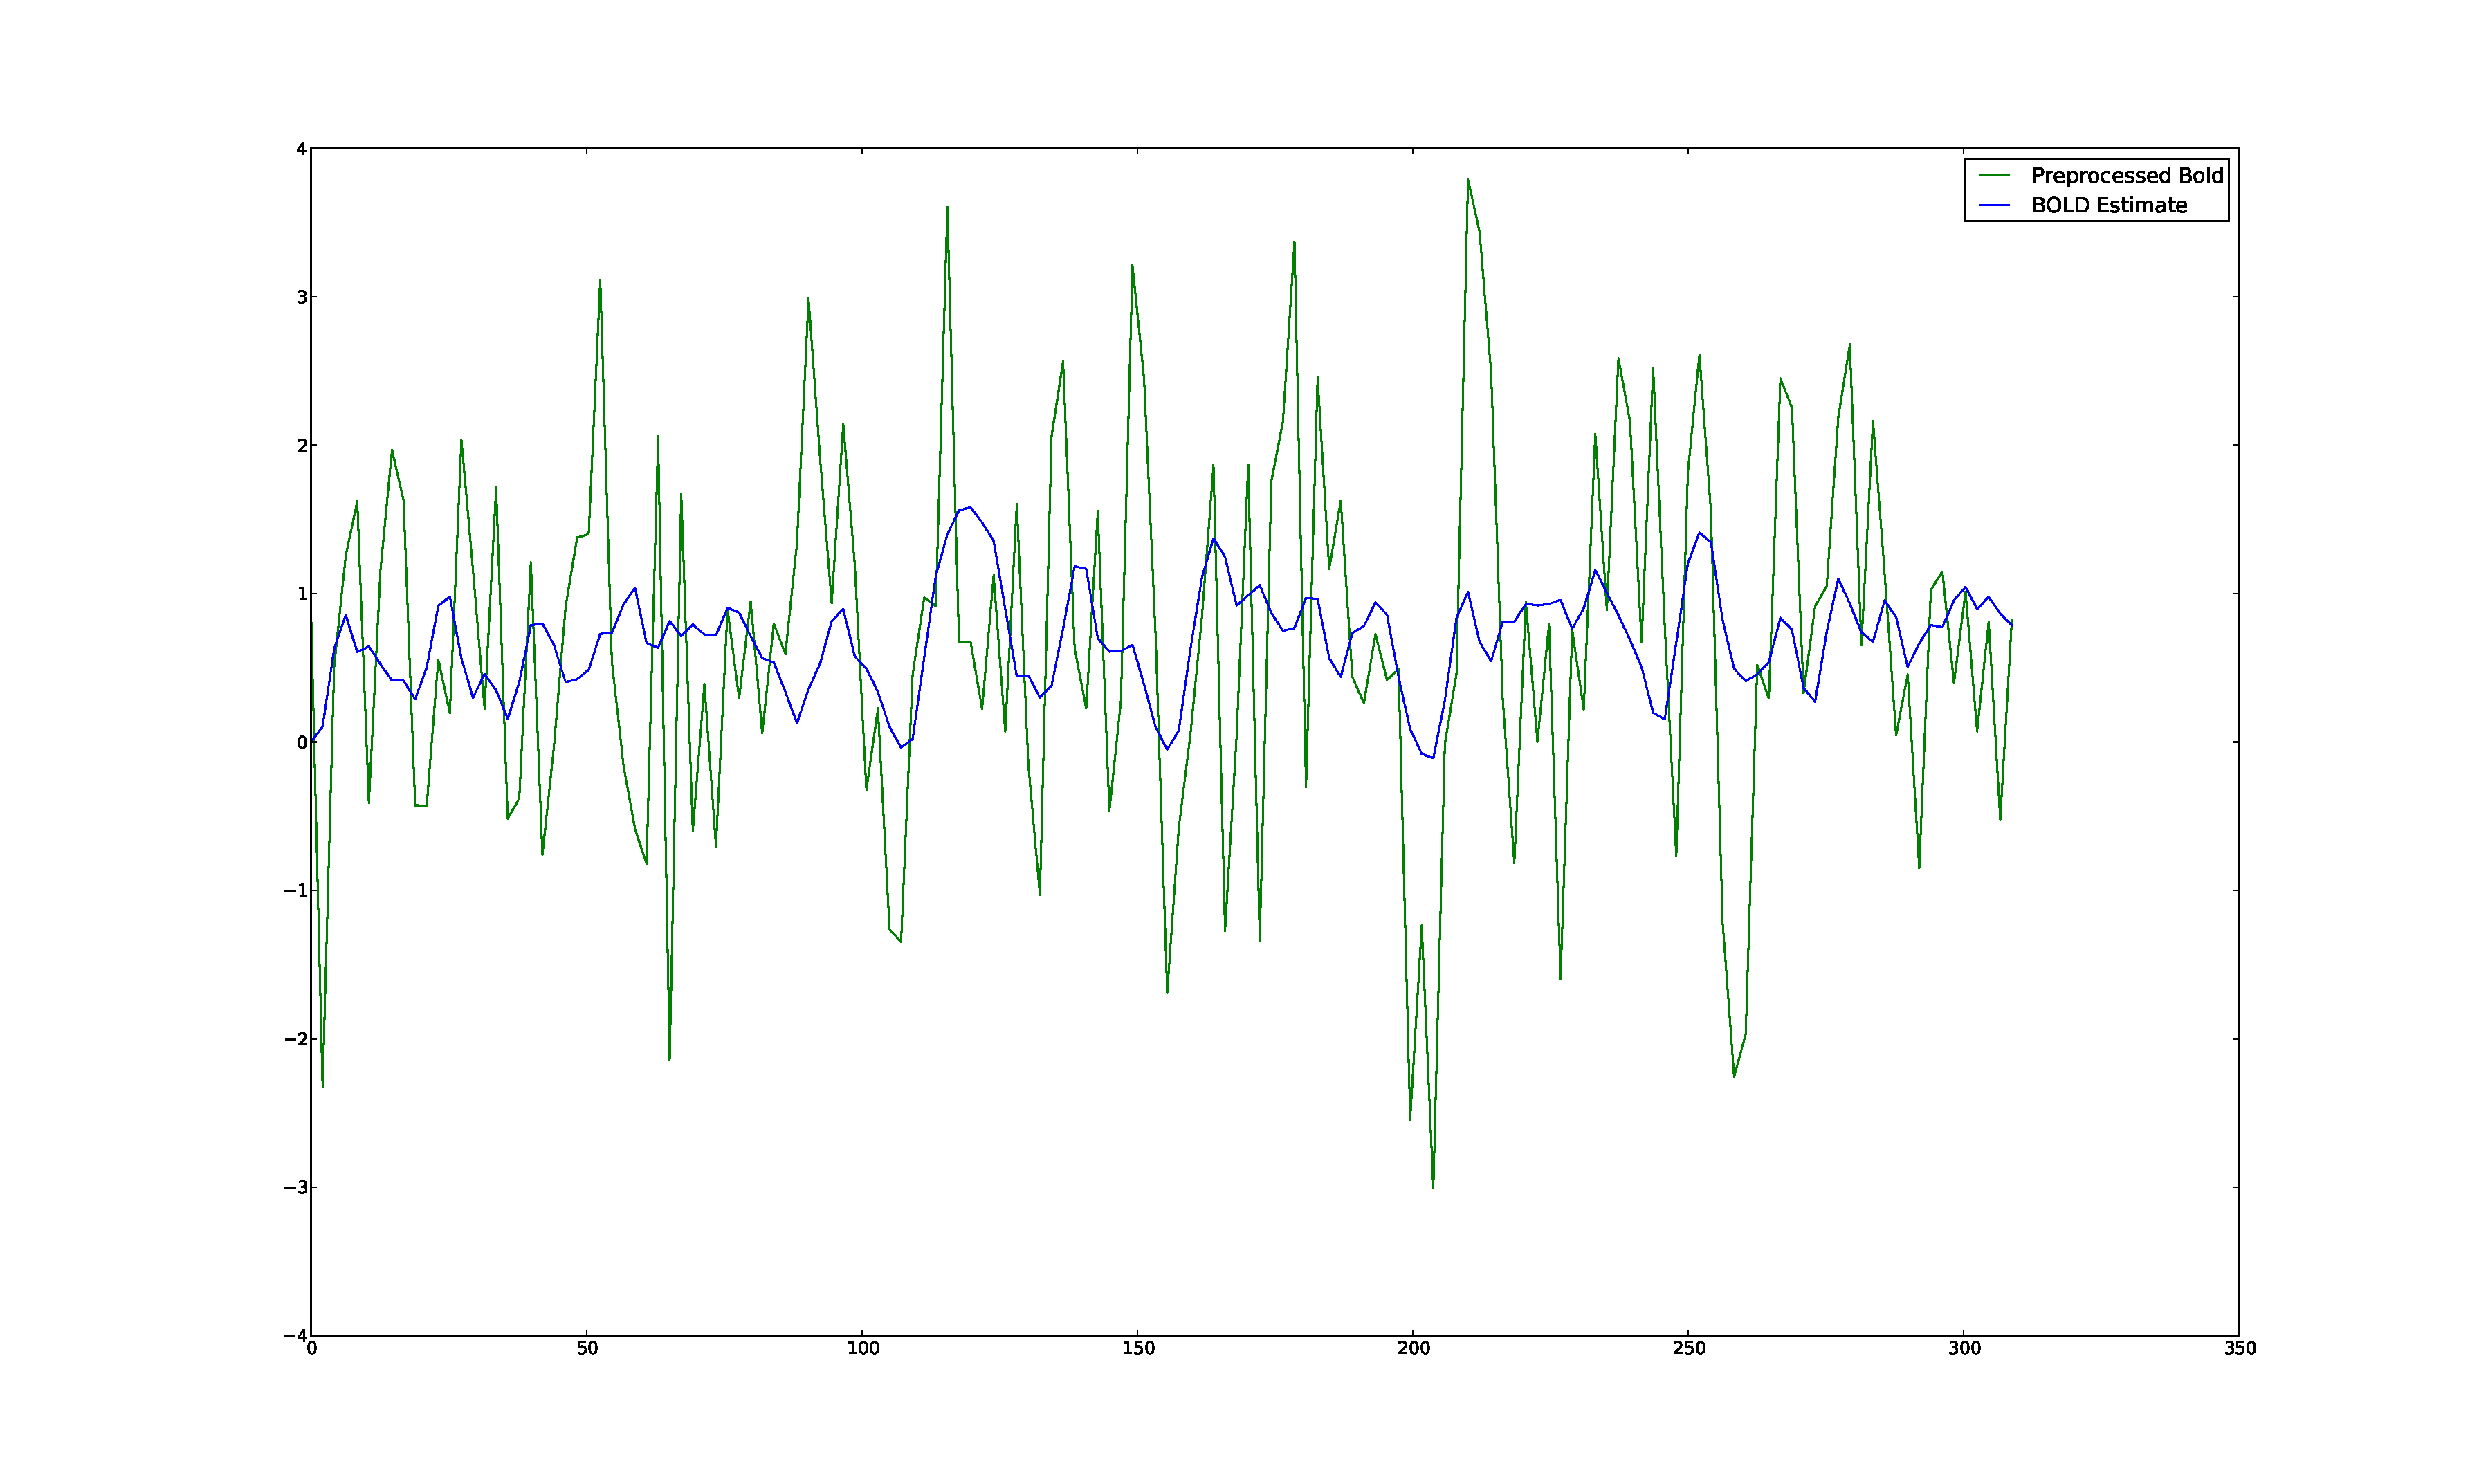
\includegraphics[clip=true,trim=5cm 1cm 4cm 1cm,width=.4\textwidth]{images/4_spm_26_15_7}}
\caption{Section 4, Estimated vs. Actual BOLD response. $t$-Score: $0.50$, Mutual Information: $0.06$, Residual: $0.95$. }
\label{fig:comp4}
\end{figure}
\end{frame}

\begin{frame}{5: 29-9-13}
\setcounter{subfigure}{0}
\begin{figure}
\centering
\subfigure[Particle Filter]{\label{fig:comp5pfilter} 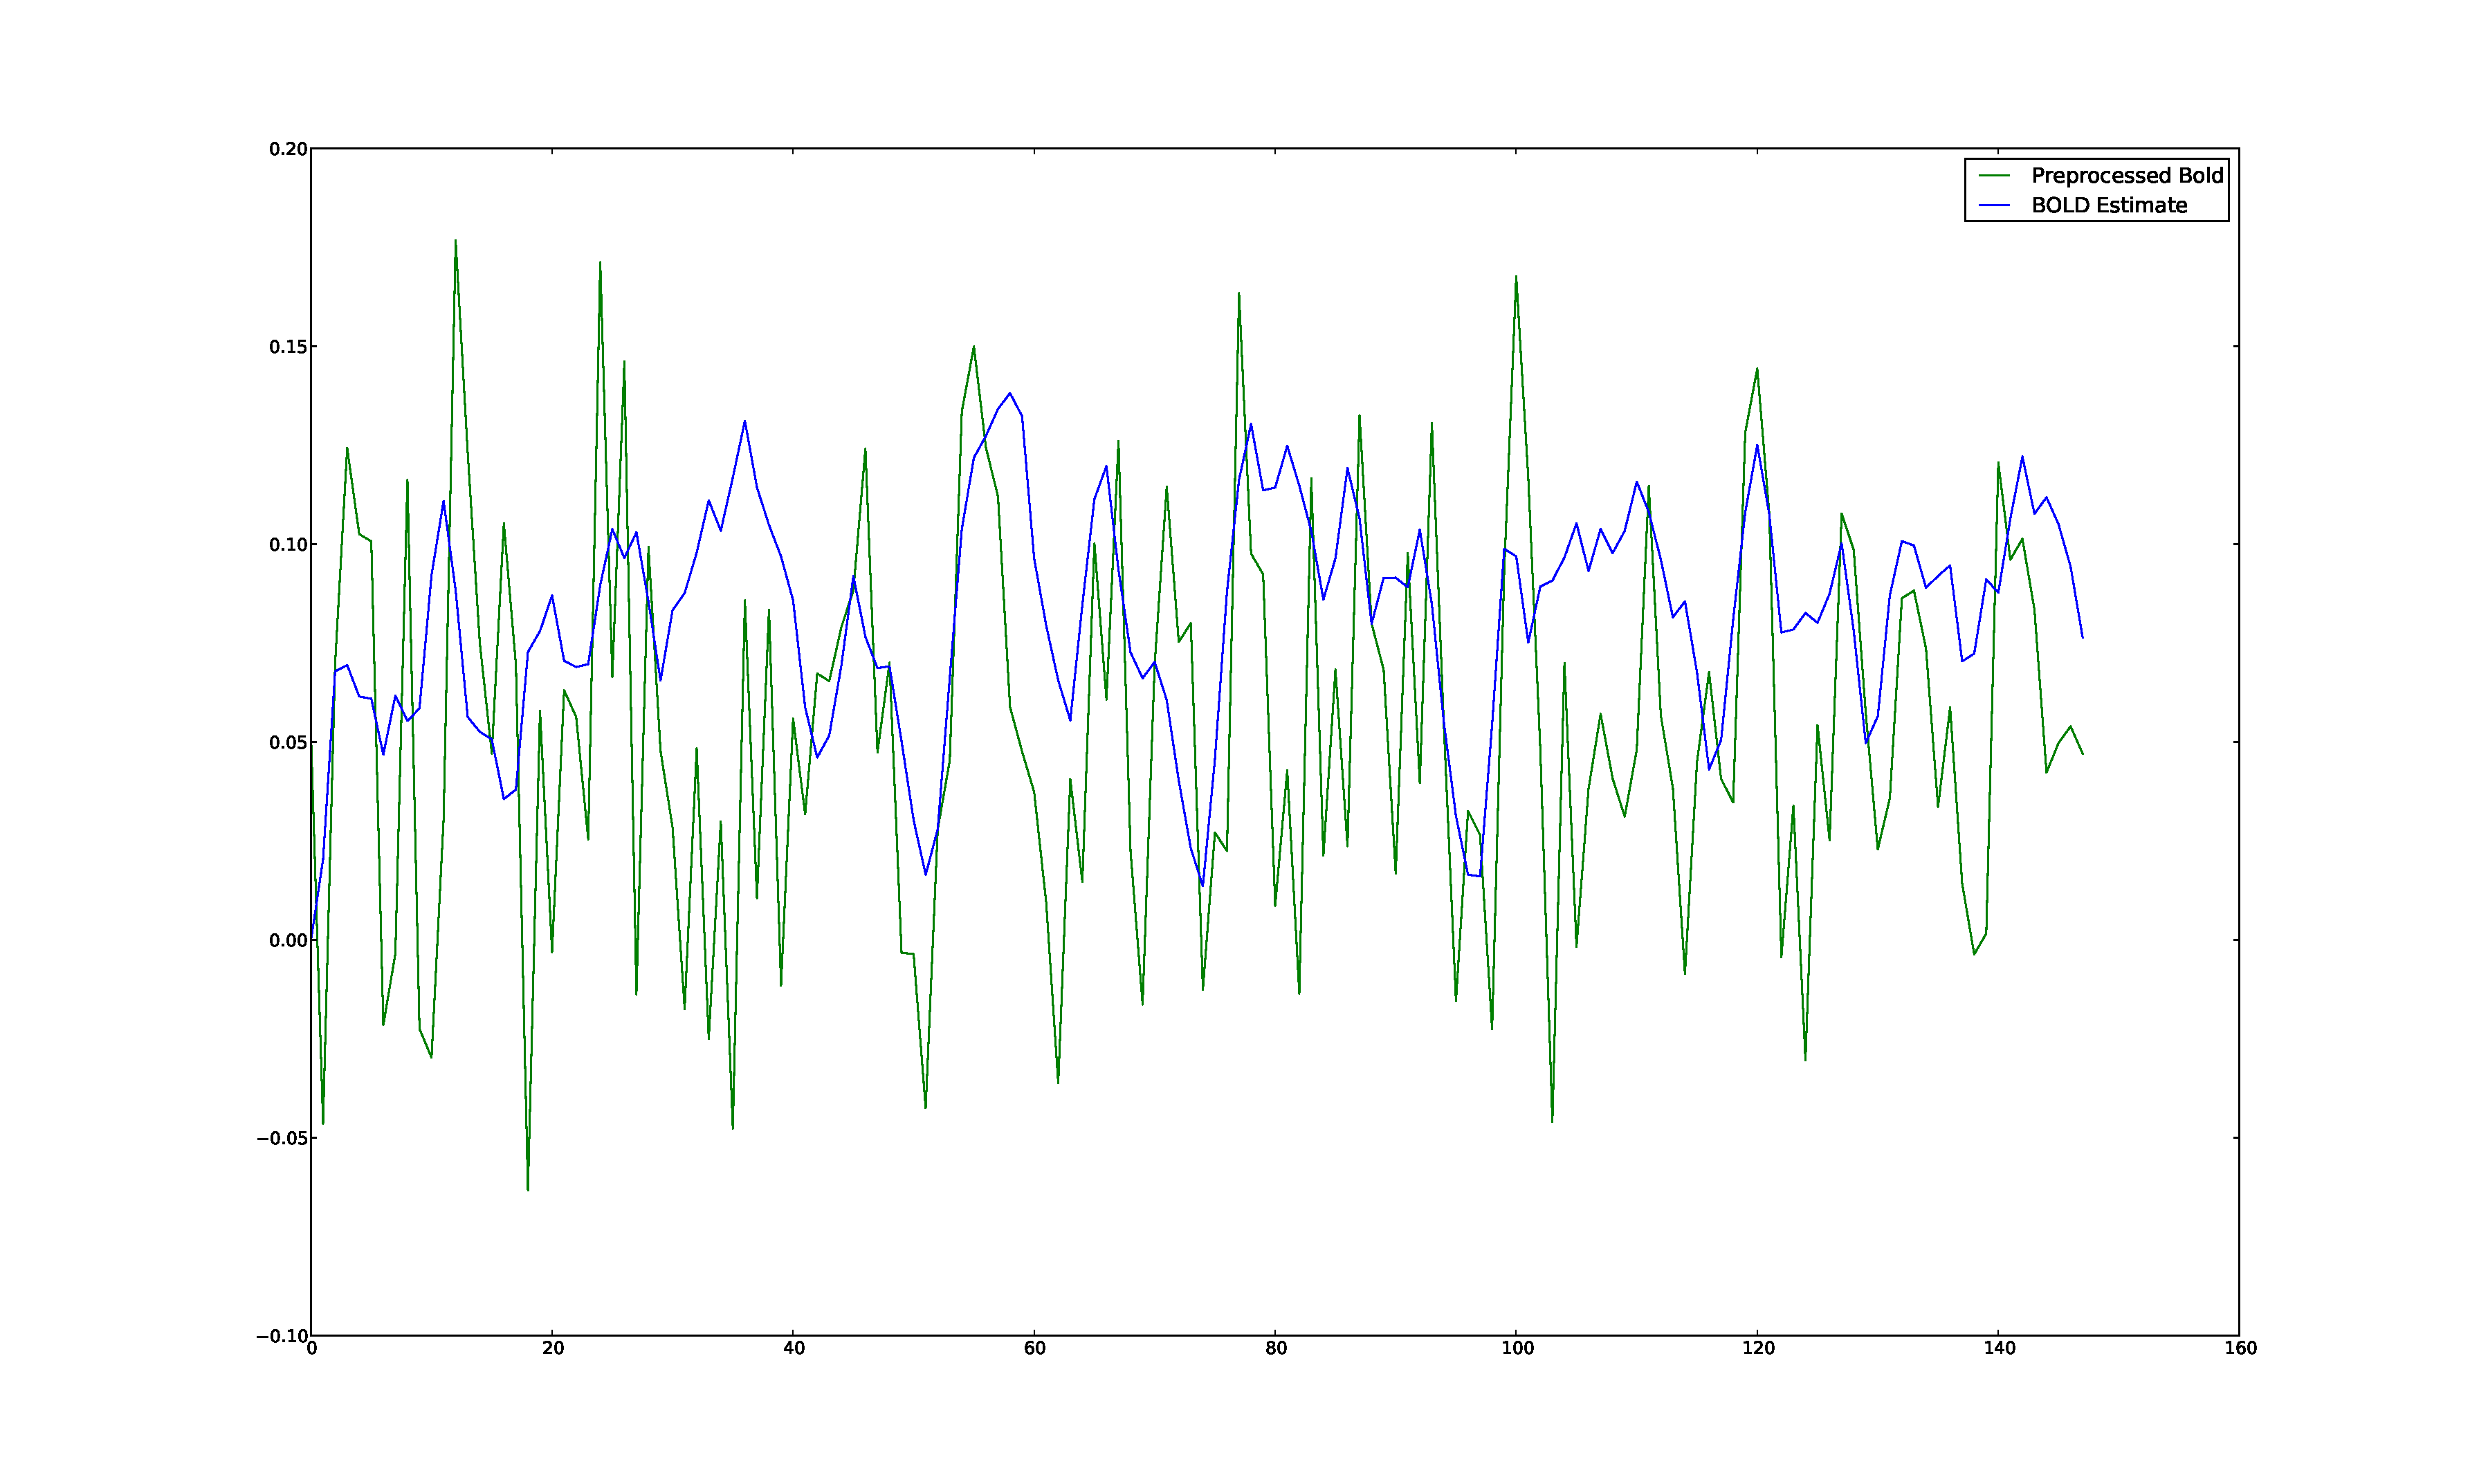
\includegraphics[clip=true,trim=5cm 1cm 4cm 1cm,width=.4\textwidth]{images/5_pfilter_29_9_13}}
\subfigure[SPM]{\label{fig:comp5spm} 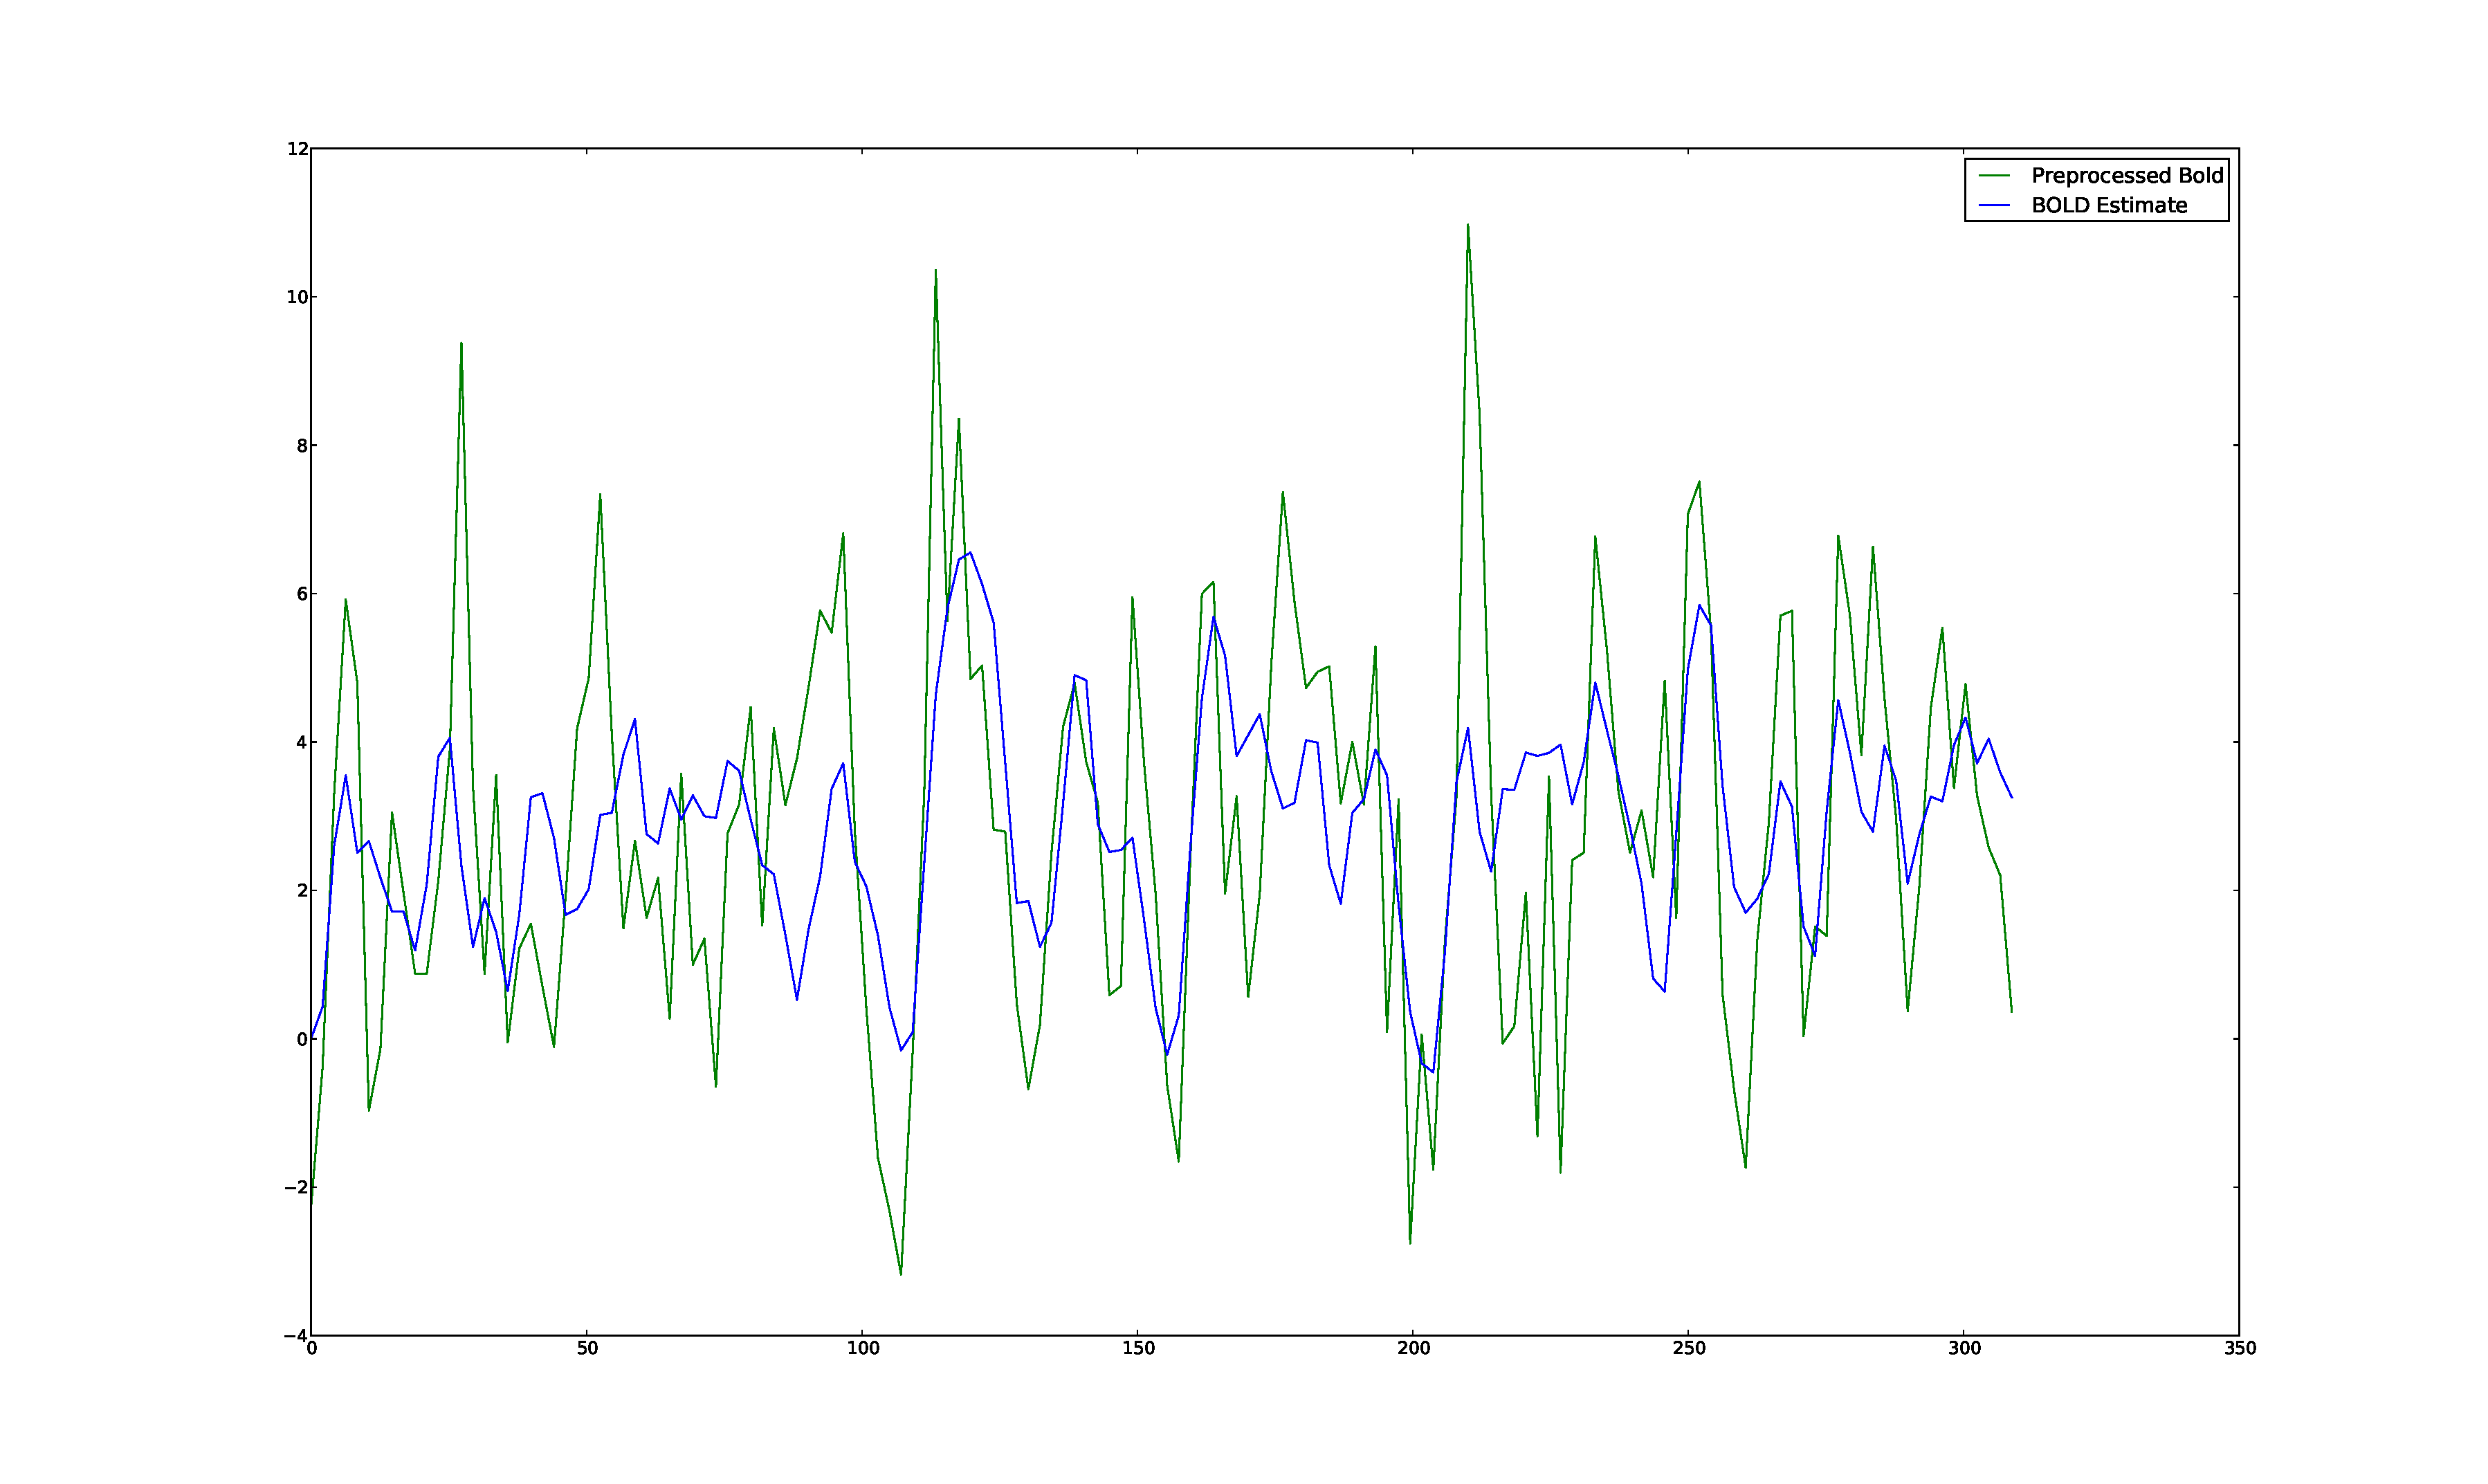
\includegraphics[clip=true,trim=5cm 1cm 4cm 1cm,width=.4\textwidth]{images/5_spm_29_9_13}}
\caption{Section 5, Estimated vs. Actual BOLD Response. $t$-Score: $4.17$, Mutual Information: $0.02$, Residual: $1.14$.}
%\caption{Section 5, Below threshold in both particle filter checks, but above threshold in SPM. Mutual Information of $0.0212822$, $t$-Value
%of $4.17399$ and $MSE$ of $1.14171$.}
\label{fig:comp5}
\end{figure}
\end{frame}

\begin{frame}{6: 36-17-19}
\setcounter{subfigure}{0}
\begin{figure}
\centering
\subfigure[Particle Filter]{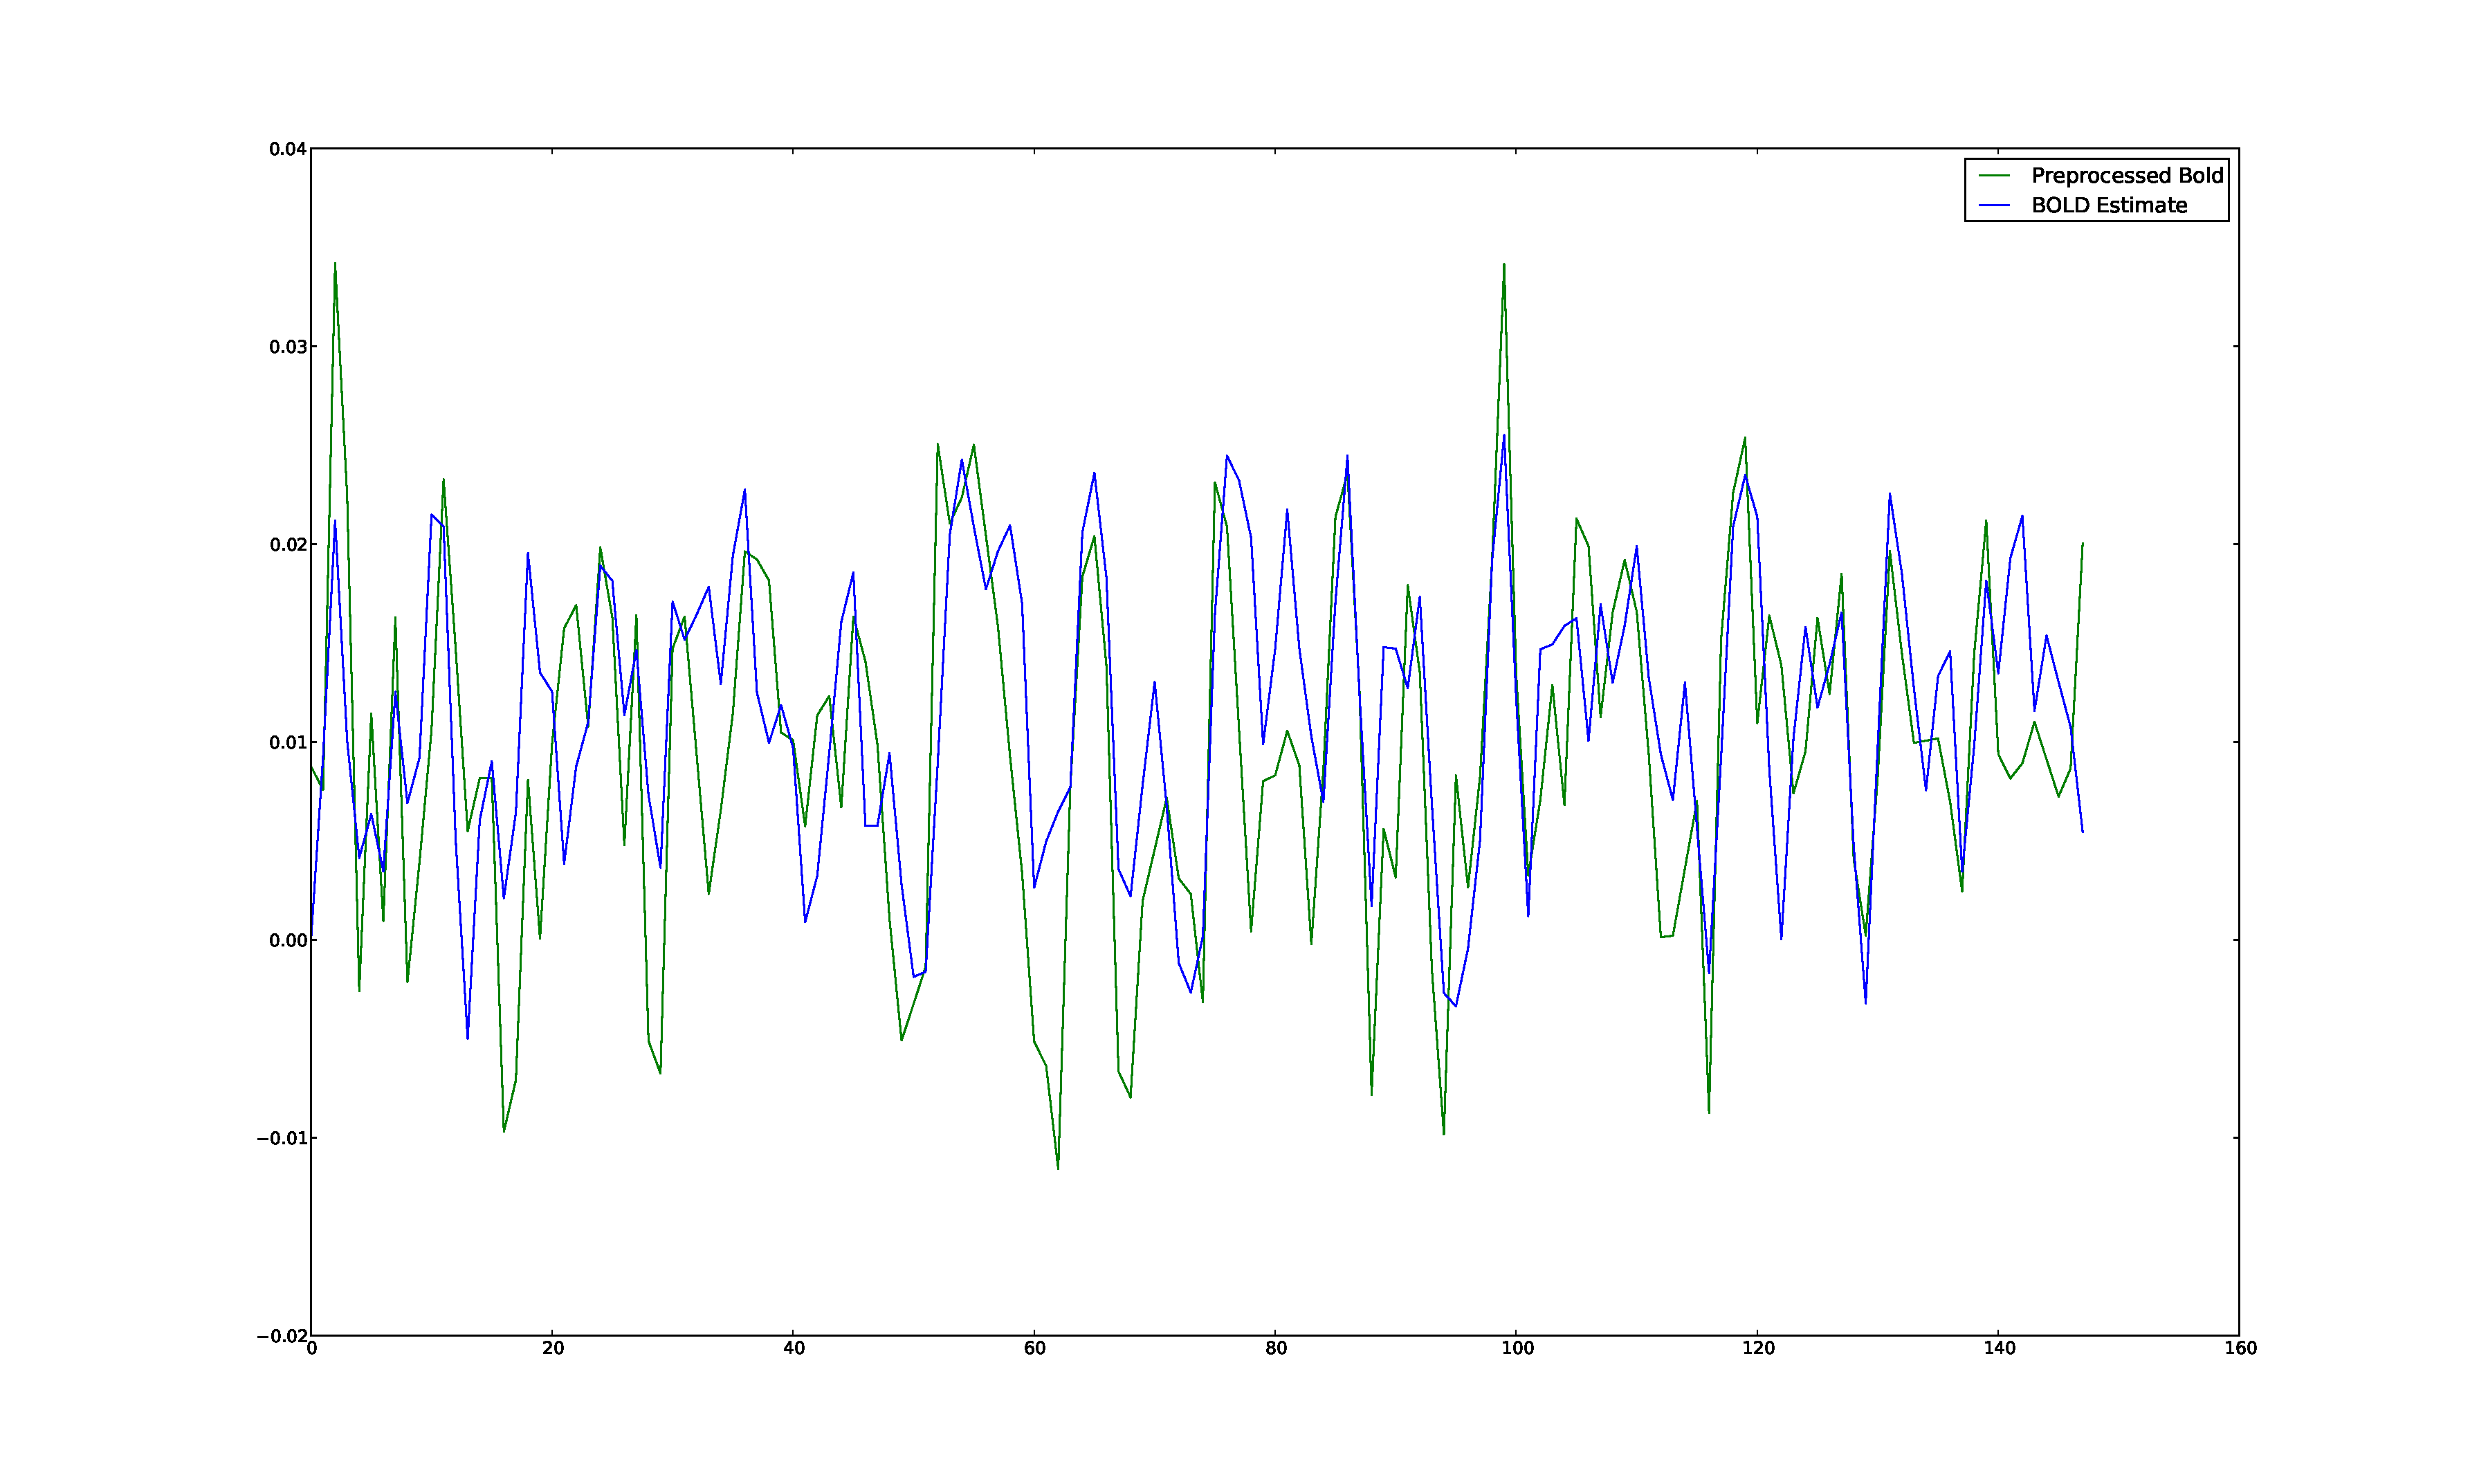
\includegraphics[clip=true,trim=5cm 1cm 4cm 1cm,width=.4\textwidth]{images/6_pfilter_36_17_19}}
\subfigure[SPM]{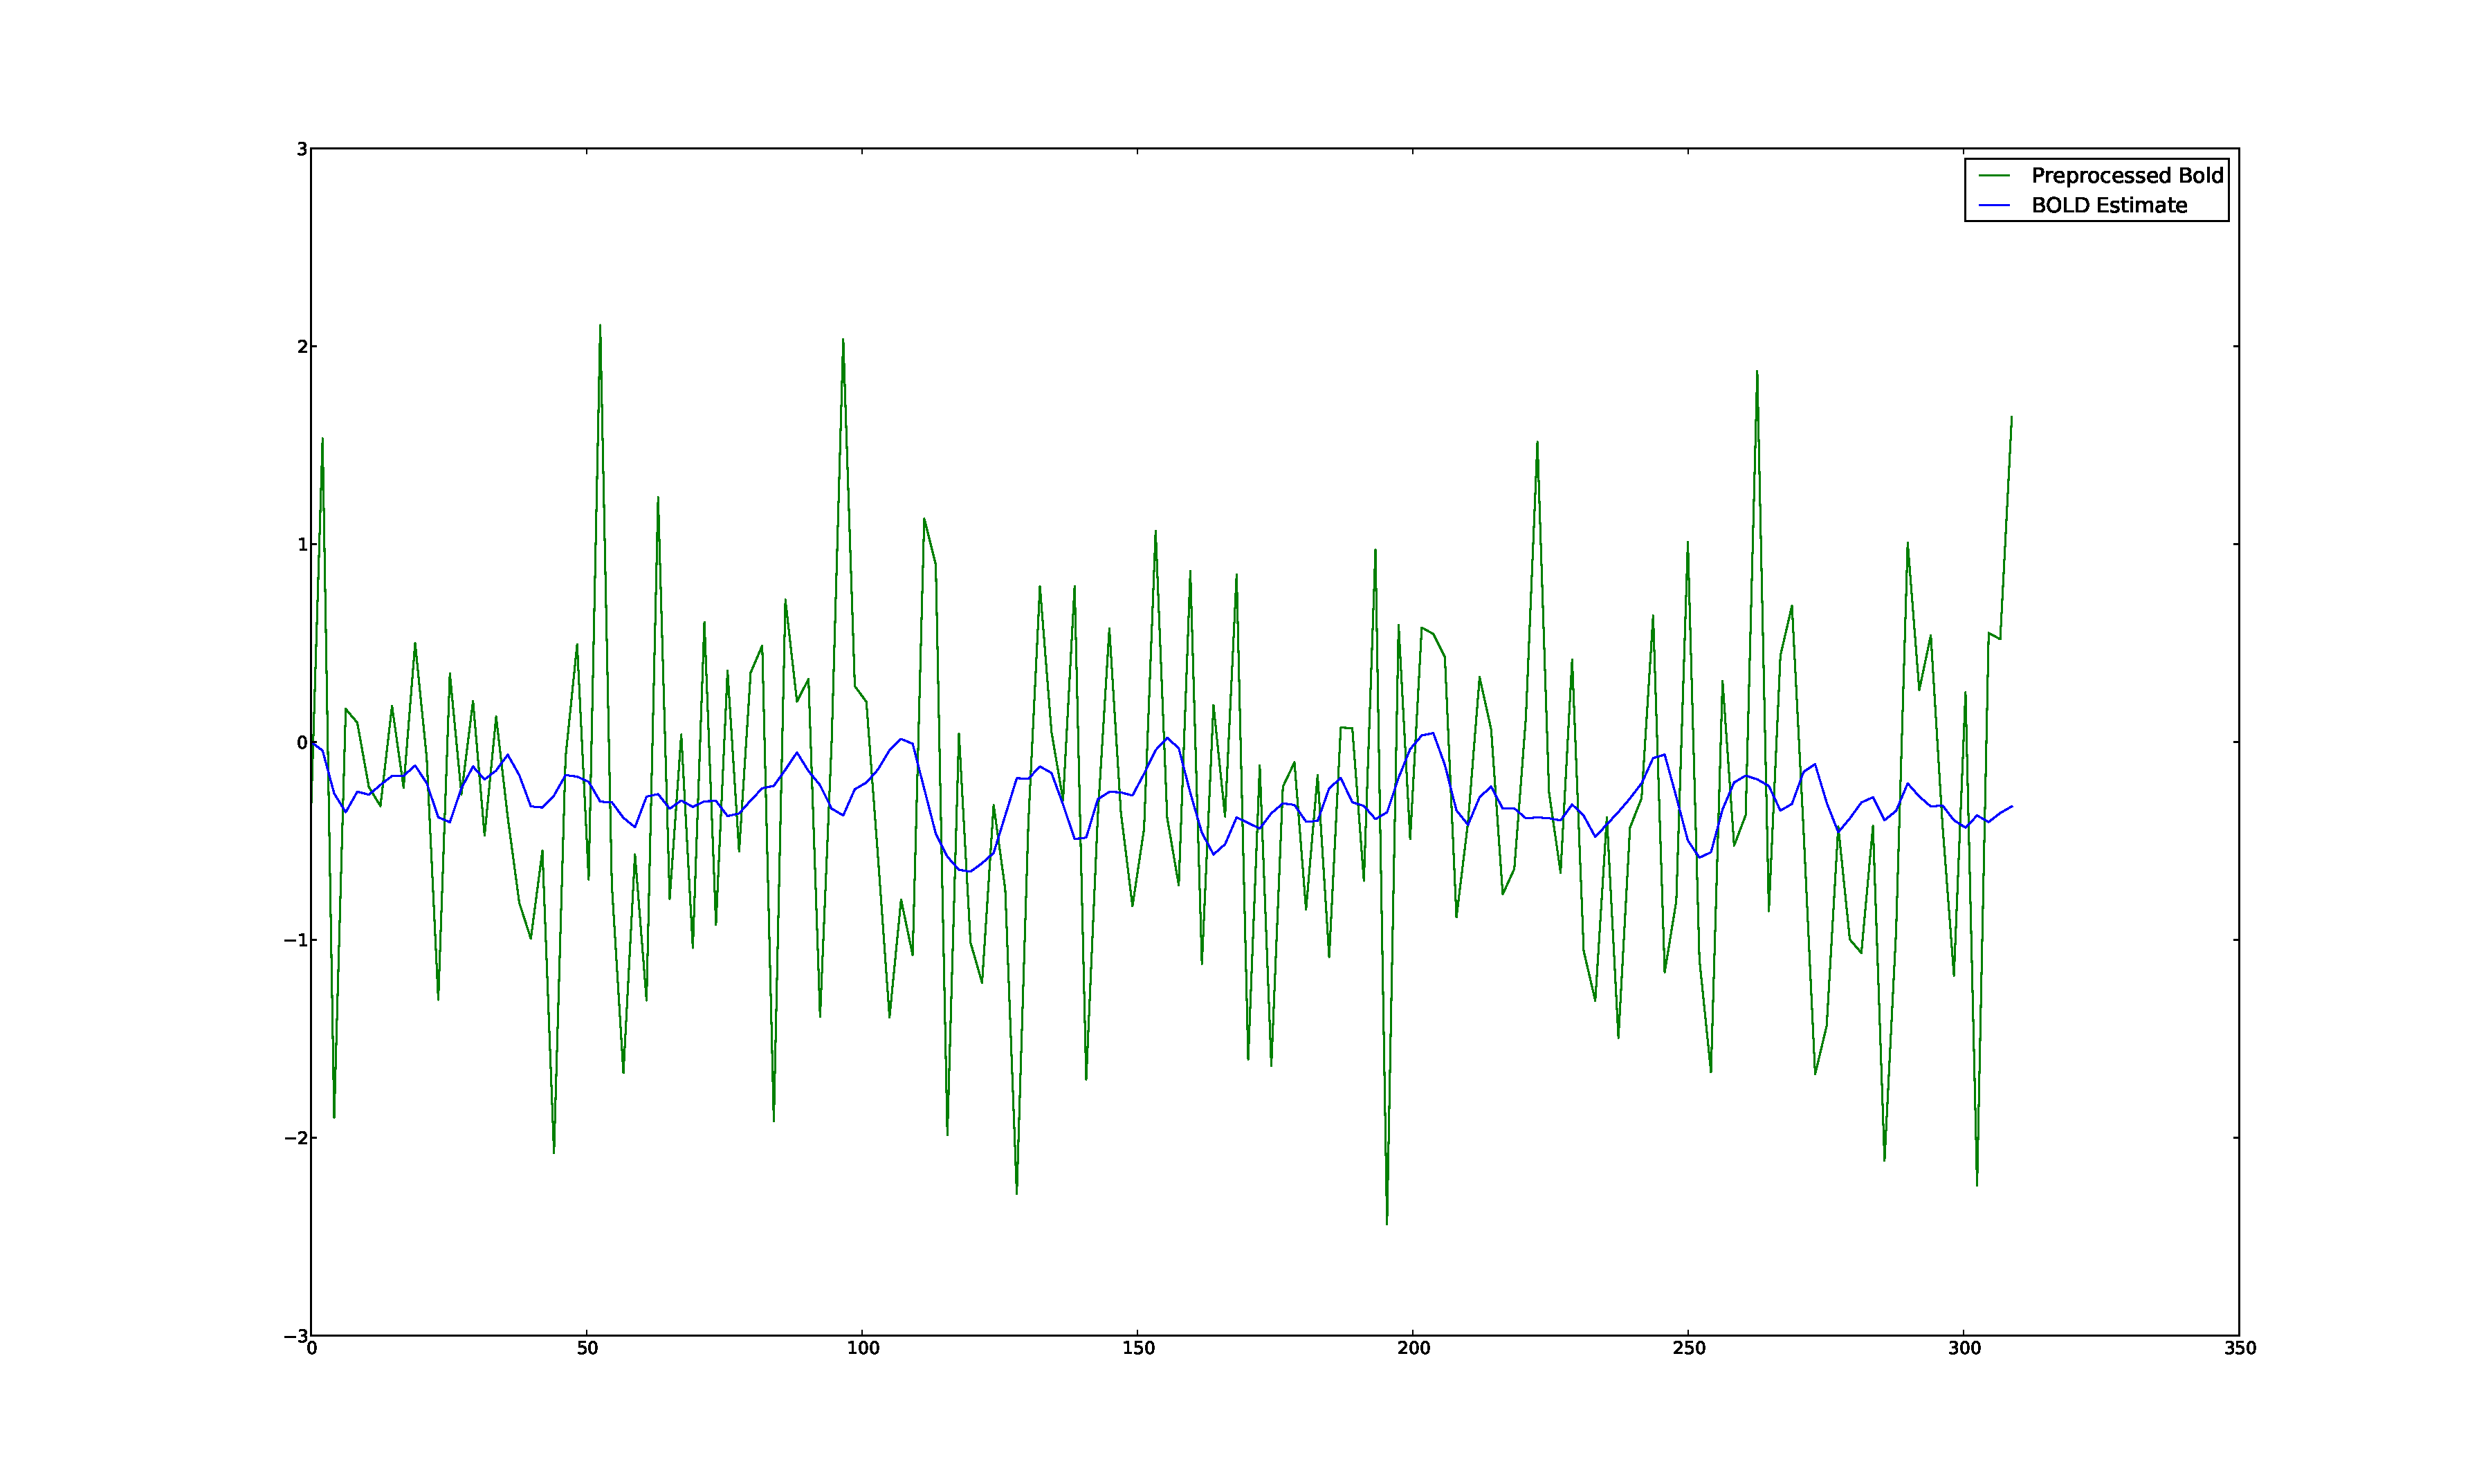
\includegraphics[clip=true,trim=5cm 1cm 4cm 1cm,width=.4\textwidth]{images/6_spm_36_17_19}}
\caption{Section 6, Estimated vs. Actual BOLD Response. $t$-Score: $2.49$, Mutual Information: $.34$, Residual: $0.78$.}
%\caption{Section 6, MI of $0.335504$, T Value: $2.49154$, normalized error: $0.783348$ Not visible in SPM}
\end{figure}
\end{frame}

\end{document}



